
\documentclass{book}
%\documentclass{book}
%If you're going to print this, perhaps get ride of oneside so that \parts{} will have their own page!
\def\title{Partial Differential Equations}
\def\author{Nathanael Chwojko-Srawley}
%\date{} % If you want to specify a date
\usepackage{inputenc}         % Used to compile any UTF-8 Character (and supports Unicode)
\usepackage{extarrows}
\usepackage{multicol} % For multiple columns
\usepackage{stackengine}
\usepackage{scalerel}
\usepackage{stackrel}         % for left-right arrows, staking symbol above and bellow
\usepackage{mathrsfs}
\usepackage{euscript}
\usepackage{makeidx}
\usepackage[font=itshape]{quoting}
\usepackage{mathtools}
\usepackage{enumitem}
\usepackage{graphicx}         % Let's you use images in LaTeX; ex the \includegraphics command.
\usepackage{wasysym}          % emoji's!
\usepackage{dsfont}
\usepackage{float}            % package with ``H'' for figures and tables, ex. Images, tables, etc
\usepackage{setspace}         % More flexibility on spacing in document.
\usepackage{commutative-diagrams}
\usepackage{hhline}
\usepackage{tikz-cd}          % for commutative diagrams https://tex.stackexchange.com/questions/419221/how-to-do-the-pushout-with-universal-property
\usepackage{longtable}        % create tables that extend past one page
\usepackage{microtype}        % makes nice text. Fixes some under-/over- filled box problems.
\usepackage{xcolor}           % Colour text.
\usepackage{wrapfig}          % To wrap text around figure
\usepackage{listings}         % Create nice colour code blocks (customized in preamble)
\usepackage{amsthm}           % Used to create theorem enviroments.
\usepackage{array}            % \begin{table}{>{\em}c c} -> 1st column italic (bfseries for bold)
\usepackage{blindtext}
\usepackage[a4paper, total={6in, 8in}]{geometry}
\usepackage{fancyhdr}
\usepackage{titlesec}
\usepackage[answerdelayed]{exercise}
\usepackage{etoolbox}          % for Dynkin diagrams
\usepackage{dynkin-diagrams}   % for Dynkin diagrams
\usepackage{pgfplots}

\usepackage{amsmath, amssymb} % Used to write better mathematical expressions (ex. \mathbb{R})
\usepackage[most]{tcolorbox} 	      % Makes nice boxes for thms, cor, prop, or anything else.
\usepackage{thmtools}         % Customize theorem environment (in preamble).
\usepackage{hyperref}
\usepackage{cleveref}


\pgfplotsset{compat=1.18}

% \usepackage{CJKutf8} % for some chinese

% \usepackage{dutchcal} % for lower case mathcal


% For citing
\usepackage{csquotes}
\usepackage{comment}
% \usepackage[backend=biber,citestyle=alphabetic,bibstyle=authortitle]{biblatex}
\usepackage{biblatex}

\addbibresource{algebra_book_cite.bib}

\providecommand{\HUGE}{\Huge}% if not using memoir
\newlength{\drop}% for my convenience
%% select a (FontSite) font by its font family ID
\newcommand*{\FSfont}[1]{\fontencoding{T1}\fontfamily{#1}\selectfont}
%% if you don’t have the FontSite fonts either \renewcommand*{\FSfont}[1]{}
%% or use your own choice of family.
%% select a (TeX Font) font by its font family ID
\newcommand*{\TXfont}[1]{\fontencoding{T1}\fontfamily{#1}\selectfont}
%% Generic publisher’s logo
\newcommand*{\plogo}{\fbox{$\mathcal{PL}$}}

%% Some shades
\definecolor{Dark}{gray}{0.2}
\definecolor{MedDark}{gray}{0.4}
\definecolor{Medium}{gray}{0.6}
\definecolor{Light}{gray}{0.8}
%%%% Additional font series macros
\makeatletter
%%%% light series
%% e.g., kernel doc, section s: line 12 or thereabouts
\DeclareRobustCommand\ltseries
{\not@math@alphabet\ltseries\relax
\fontseries\ltdefault\selectfont}
%% e.g., kernel doc, section t: line 32 or thereabouts
\newcommand{\ltdefault}{l}
%% e.g., kernel doc, section v: line 19 or thereabouts
\DeclareTextFontCommand{\textlt}{\ltseries}
% heavy(bold) series
\DeclareRobustCommand\hbseries
{\not@math@alphabet\hbseries\relax
\fontseries\hbdefault\selectfont}
\newcommand{\hbdefault}{hb}
\DeclareTextFontCommand{\texthb}{\hbseries}
\makeatother


\newcommand{\titleUL}{\begingroup% University of Liege
\drop=0.1\textheight
\vspace*{\drop}
\begin{center}
% {\LARGE\textsc{University of Toronto}}\\[\drop]
% University logo
% {\LARGE \plogo}\\[\drop]
{\LARGE {\quad}}\\[\drop]

\rule{\textwidth}{1pt}\par
\vspace{0.5\baselineskip}
{\huge\bfseries \title\\[0.2\baselineskip]
\large --- \emph{EYNTKA} Series ---}\\[0.5\baselineskip]
\rule{\textwidth}{1pt}\par
\vfill
{\Large\textsc{\author}}
\vfill
\vfill
{\large \today}
\end{center}
\endgroup}

%header information
\pagestyle{fancy}
\setlength\headheight{20pt}
\renewcommand{\sectionmark}[1]{\markright{\thesection.\ #1}}
\renewcommand{\chaptermark}[1]{\markboth{#1}{}}
\fancyfoot[C,CO]{\textcolor{gray}{Nathanael Chwojko-Srawley}}
\fancyfoot[R,RO]{\thepage}{}

\titleformat
{\chapter} % command
[display] % shape
{\bfseries\Huge\itshape} % format
{\thechapter} % label
{0.5ex} % sep
{
    \rule{\textwidth}{1pt}
    \vspace{2ex}
    \centering
} % before-code
[
\vspace{-0.5ex}%
\rule{\textwidth}{1pt}
] % after-code

% Create a new page style for the first page
\fancypagestyle{firstpage}{
  \fancyhf{} % Clear header and footer
  \renewcommand{\headrulewidth}{0pt} % This removes the header line
  \fancyfoot[C]{\thepage}
}

% Apply the first page style conditionally
\AtBeginDocument{\thispagestyle{firstpage}}


\stackMath %to be able to stack text in math mode
% For devnagari font for that one example




%\ExerciseLevelInToc
\counterwithin{Exercise}{section}
\counterwithin{Answer}{section}
%\renewcommand{\ExerciseHeader}{\noindent\def\stackalignment{c}% code from https://tex.stackexchange.com/a/195118/101651
    %\stackunder{{\textbf{\large\ExerciseName}}}{\textcolor{black}{\rule{40pt}{4pt}}}\medskip}



%theorem code
\definecolor{dkgreen}{rgb}{0,0.6,0}
\definecolor{gray}{rgb}{0.5,0.5,0.5}
\definecolor{mauve}{rgb}{0.58,0,0.82}
\definecolor{lightyellow}{rgb}{1,1,0.6}
\definecolor{reddish}{HTML}{A01A3A}
%Theorems, propositions, Corollaries, Definitions

% breakable,

%Wanna implement this, but not working: https://tex.stackexchange.com/questions/547979/problem-numbering-environment
\newtcbtheorem[number within=section]{thm}{Theorem}%
{
colback=green!5,
colframe=green!35!black,
fonttitle=\bfseries,
label type=theorem
}{th}

\newtcbtheorem[number within=section, use counter from=thm]{lem}{Lemma}%
{
colback=blue!5,
colframe=black!35!black,
fonttitle=\bfseries,
label type=lemma
}{lm}
\newtcbtheorem[number within=section, use counter from=thm]{prop}{Proposition}%
{
colback=white!5,
colframe=white!35!black,
fonttitle=\bfseries,
label type=proposition
}{pr}
\newtcbtheorem[number within=section, use counter from=thm]{cor}{Corollary}%
{colback=blue!5,
colframe=blue!35!black,
fonttitle=\bfseries,
label type=corollary
}{co}
\newtcbtheorem[number within=section, use counter from=thm]{axiom}{Axiom}%
{colback=black!5,
colframe=yellow!35!black,
fonttitle=\bfseries,
label type=axiom
}{ax}
\newtcbtheorem[number within=section, use counter from=thm]{defn}{Definition}%
{colback=red!5,
colframe=red!35!black,
fonttitle=\bfseries,
label type=definition
}{df}


% for <s-cr> to create \item[$\LRw$] instead of \item
\newenvironment{equivEnumerate}
 {\begin{enumerate}
	}{
\end{enumerate}}

\newtcbtheorem[number within=section, use counter from=thm]{titledBox}{}{%
  enhanced,
  sharp corners,
  colback=white,
  colframe=black,
  borderline={0.2pt}{0pt}{black},
  left=2mm,
  right=2mm,
  top=2mm,
  bottom=2mm,
  title style={opacity=1},
  attach title to upper,
  before upper={\textbf{\tcbtitletext}\quad},
  coltitle=black,
  fonttitle=\bfseries,
  separator sign={\quad}
}{box}


%better example and proof environments
\def\exampletext{Example} % If English
\colorlet{colexam}{red!55!black} % Global example color


\newtcbtheorem[number within=section, use counter from=thm]{example}{Example}{% \newtcolorbox[use counter=testexample]{testexamplebox}{%
% Example Frame Start
empty,% Empty previously set parameters
title={\exampletext \thetcbcounter #1},% use \thetcbcounter to access the testexample counter text
% Attaching a box requires an overlay
attach boxed title to top left,
   % Ensures proper line breaking in longer titles
   minipage boxed title,
% (boxed title style requires an overlay)
boxed title style={empty,size=minimal,toprule=0pt,top=4pt,left=3mm,overlay={}},
coltitle=colexam,fonttitle=\bfseries,
before=\par\medskip\noindent,parbox=false,boxsep=0pt,left=3mm,right=0mm,top=2pt,breakable,pad at break=0mm,
   before upper=\csname @totalleftmargin\endcsname0pt, % Use instead of parbox=true. This ensures parskip is inherited by box.
% Handles box when it exists on one page only
overlay unbroken={\draw[colexam,line width=.5pt] ([xshift=-0pt]title.north west) -- ([xshift=-0pt]frame.south west); },
% Handles multipage box: first page
overlay first={\draw[colexam,line width=.5pt] ([xshift=-0pt]title.north west) -- ([xshift=-0pt]frame.south west); },
% Handles multipage box: middle page
overlay middle={\draw[colexam,line width=.5pt] ([xshift=-0pt]frame.north west) -- ([xshift=-0pt]frame.south west); },
% Handles multipage box: last page
overlay last={\draw[colexam,line width=.5pt] ([xshift=-0pt]frame.north west) -- ([xshift=-0pt]frame.south west); }%
}{ex}



\newtcolorbox{ProofTcb}[1][]{%
    empty,
    title={\emph{Proof}: #1},
    attach boxed title to top left,
    minipage boxed title,
    boxed title style={empty,size=minimal,toprule=0pt,top=4pt,left=3mm,overlay={}},
    coltitle=black!55!black,
    fonttitle=\bfseries,
    before=\par\medskip\noindent,
    parbox=false,
    boxsep=0pt,
    left=3mm,
    right=0mm,
    top=2pt,
    breakable,
    pad at break=0mm,
    before upper=\csname @totalleftmargin\endcsname0pt,
    width=\dimexpr\textwidth-3mm\relax,
    overlay unbroken={\draw[black!55!black,line width=.5pt] ([xshift=-0pt]title.north west) -- ([xshift=-0pt]frame.south west); },
    overlay first={\draw[black!55!black,line width=.5pt] ([xshift=-0pt]title.north west) -- ([xshift=-0pt]frame.south west); },
    overlay middle={\draw[black!55!black,line width=.5pt] ([xshift=-0pt]frame.north west) -- ([xshift=-0pt]frame.south west); },
    overlay last={\draw[black!55!black,line width=.5pt] ([xshift=-0pt]frame.north west) -- ([xshift=-0pt]frame.south west); },
    #1
}

\newenvironment{Proof}[1][]
  {\begin{ProofTcb}[#1]}
  {\end{ProofTcb}}


%shortcuts for this file (newcommand and renewcommand)

% I like original mathcal better, but need lowercase.
\DeclareFontFamily{OT1}{pzc}{}
\DeclareFontShape{OT1}{pzc}{m}{it}{<-> s * [1.10] pzcmi7t}{}
\DeclareMathAlphabet{\mathpzc}{OT1}{pzc}{m}{it}

% Custom Commands
\newcommand{\A}{{\mathbb{A}}}
\newcommand{\F}{{\mathbb{F}}}
\newcommand{\N}{{\mathbb{N}}}
\newcommand{\Q}{{\mathbb{Q}}}
\newcommand{\R}{{\mathbb{R}}}
\newcommand{\V}{{\mathbb{V}}}
\newcommand{\Z}{{\mathbb{Z}}}
\newcommand{\C}{{\mathbb{C}}}
\renewcommand{\P}{{\mathbb{P}}}
\renewcommand{\H}{{\mathbb{H}}}

\newcommand{\CA}{{\mathcal{A}}}
\newcommand{\CB}{{\mathcal{B}}}
\newcommand{\CC}{{\mathcal{C}}}
\newcommand{\CD}{{\mathcal{D}}}
\newcommand{\CF}{{\mathcal{F}}}
\newcommand{\CG}{{\mathcal{G}}}
\newcommand{\CH}{{\mathcal{H}}}
\newcommand{\CI}{{\mathcal{I}}}
\newcommand{\CL}{{\mathcal{L}}}
\newcommand{\CN}{{\mathcal{N}}}
\newcommand{\CO}{{\mathcal{O}}}
\newcommand{\co}{{\mathpzc{o}}}
\newcommand{\CP}{{\mathbb{C}\mathrm{P}}}
\newcommand{\RP}{{\mathbb{R}\mathrm{P}}}
\newcommand{\CQ}{{\mathcal{Q}}}
\newcommand{\CR}{{\mathcal{R}}}
\newcommand{\CK}{{\mathcal{K}}}
\newcommand{\CS}{{\mathcal{S}}}
\newcommand{\CT}{{\mathcal{T}}}
\newcommand{\CV}{{\mathcal{V}}}
\newcommand{\CZ}{{\mathcal{Z}}}
\newcommand{\ff}{{\mathscr{F}}}
\newcommand{\EF}{{\EuScript{F}}}
\newcommand{\EL}{{\EuScript{L}}}
\newcommand{\EO}{{\EuScript{O}}}
\newcommand{\EC}{{\EuScript{C}}}
\newcommand{\fo}{{\mathfrak{o}}}
\newcommand{\fa}{{\mathfrak{a}}}
\newcommand{\fb}{{\mathfrak{b}}}
\newcommand{\fc}{{\mathfrak{c}}}
\newcommand{\fd}{{\mathfrak{d}}}
\newcommand{\fm}{{\mathfrak{m}}}
\newcommand{\fn}{{\mathfrak{n}}}
\newcommand{\fp}{{\mathfrak{p}}}
\newcommand{\fq}{{\mathfrak{q}}}
\newcommand{\FA}{{\mathfrak{A}}}
\newcommand{\FB}{{\mathfrak{B}}}
\newcommand{\FP}{{\mathfrak{P}}}
\newcommand{\FC}{{\mathfrak{C}}}
\newcommand{\FD}{{\mathfrak{D}}}
\newcommand{\FM}{{\mathfrak{M}}}
\newcommand{\FN}{{\mathfrak{N}}}
\newcommand{\FO}{{\mathfrak{O}}}



\newcommand{\sse}{\subseteq}
\newcommand{\nsse}{\not\subseteq}
\newcommand{\ssne}{\subsetneq}
\newcommand{\qn}{\quad\newline}
\newcommand{\placeholder}{\_\_\_\_\_}
\newcommand{\subg}{\leqslant}
%\newcommand{\subgne}{\lneqslant}
\newcommand{\supg}{\geqslant}
\newcommand{\nsubg}{\trianglelefteq}
\newcommand{\csubg}{\blacktriangleleft}
\newcommand{\nsupg}{\trianglerighteq}
\newcommand{\isosubg}{\lesssim}
\renewcommand{\mid}{\big|}
\renewcommand{\phi}{\varphi}

\newcommand{\oln}[1]{{\overline{#1}}}
\renewcommand{\bf}[1]{\textbf{#1}}

\renewcommand{\mod}{\,\operatorname{mod}\,}

\newcommand{\ev}{{\operatorname{ev}}}
\newcommand{\tr}{{\operatorname{tr}}}
\newcommand{\nm}{{\operatorname{Nm}}}
\newcommand{\op}{{\operatorname{op}}}
\newcommand{\ad}{{\operatorname{ad}}}
\newcommand{\rk}{{\operatorname{rk}}}
\newcommand{\im}{{\operatorname{im}}}
\newcommand{\id}{{\operatorname{id}}}
\newcommand{\ch}{{\operatorname{ch}}}
\newcommand{\ab}{{\operatorname{ab}}}
\newcommand{\Ch}{{\operatorname{Ch}}}
\newcommand{\Br}{{\operatorname{Br}}}
\newcommand{\Ab}{{\operatorname{Ab}}}
\newcommand{\SL}{{\operatorname{SL}}}
\newcommand{\GL}{{\operatorname{GL}}}
\newcommand{\rad}{\operatorname{rad}}
\newcommand{\sep}{\operatorname{sep}}
\newcommand{\vol}{\operatorname{vol}}
\newcommand{\ord}{\operatorname{ord}}
\newcommand{\Gal}{\operatorname{Gal}}
\newcommand{\Rep}{\operatorname{Rep}}
\newcommand{\Aut}{\operatorname{Aut}}
\newcommand{\Sym}{\operatorname{Sym}}
\newcommand{\Mod}[1][]{{}_{#1}\operatorname{Mod}}
\newcommand{\RMod}{{}_R\operatorname{Mod}}
\newcommand{\Grp}{{\textbf{Grp}}}
\newcommand{\Alg}{{\textbf{Alg}}}
\newcommand{\Set}{{\textbf{Set}}}
\newcommand{\Fld}{{\textbf{Fld}}}
\newcommand{\AlgInt}{{\textbf{AlgInt}}}
\newcommand{\fin}{{\operatorname{fin}}}
\newcommand{\Pic}{{\operatorname{Pic}}}
\newcommand{\Div}{{\operatorname{Div}}}
\newcommand{\Hom}{{\operatorname{Hom}}}
\newcommand{\Emb}{{\operatorname{Emb}}}
\newcommand{\Ext}{{\operatorname{Ext}}}
\newcommand{\End}{{\operatorname{End}}}
\newcommand{\Inn}{{\operatorname{Inn}}}
\newcommand{\Int}{{\operatorname{int}}}
\newcommand{\Irr}{{\operatorname{Irr}}}
\newcommand{\Ind}{{\operatorname{Ind}}}
\newcommand{\Out}{{\operatorname{Out}}}
\newcommand{\Jac}{{\operatorname{Jac}}}
\newcommand{\Nil}{{\operatorname{Nil}}}
\newcommand{\Tor}{{\operatorname{Tor}}}
\newcommand{\Top}{{\operatorname{Top}}}
\newcommand{\Ann}{{\operatorname{Ann}}}
\newcommand{\Syl}{{\operatorname{Syl}}}
\newcommand{\Res}{{\operatorname{Res}}}
\newcommand{\lcm}{{\operatorname{lcm}}}
\newcommand{\conj}{{\operatorname{conj}}}
\newcommand{\disc}{{\operatorname{disc}}}
\newcommand{\stab}{{\operatorname{stab}}}
\newcommand{\kdim}{{\operatorname{kdim}}}
\newcommand{\diag}{{\operatorname{diag}}}
\newcommand{\coker}{{\operatorname{coker}}}
\newcommand{\Obj}{{\operatorname{Obj}}}
\newcommand{\Mor}[1]{\operatorname{Mor}(\textbf{#1})}
\newcommand{\Frac}{{\operatorname{Frac}}}
\newcommand{\Frob}{{\operatorname{Frob}}}
\newcommand{\Spec}{{\operatorname{Spec}}}
\newcommand{\mSpec}{{\operatorname{mSpec}}}
\newcommand{\Tens}[1]{#1\otimes \_\_}
\newcommand{\Char}{{\operatorname{char}}}
\newcommand{\Span}{{\operatorname{span}}}
\newcommand{\Lim}{{\varprojlim}}
\newcommand{\colim}{\varinjlim}
\newcommand{\coLim}{{\varinjlim}}
\newcommand{\Dlim}{\lim\limits_{\longrightarrow}}
\newcommand{\coDlim}{\lim\limits_{\longleftarrow}}
\newcommand{\codim}{{\operatorname{codim}}}
\newcommand{\fHom}[1]{\operatorname{Hom}(#1, \_\_)}
\newcommand{\cofHom}[1]{\operatorname{Hom}(\_\_, #1)}
\newcommand{\trdeg}{{\operatorname{trdeg}}}
\newcommand{\acton}{\curvearrowright}
\newcommand{\actson}{\curvearrowright}

\renewcommand{\Re}{{\operatorname{Re}}}
\renewcommand{\Im}{{\operatorname{Im}}}

%for saturated ideals in the localization section
\newcommand{\LIm}{{}^{\iota} }
\newcommand{\LPre}{{}^{\pi} }

% Arrows
\newcommand{\rw}{\rightarrow}
\newcommand{\rrw}{\rightrightarrows}
\newcommand{\Rw}{\Rightarrow}
\newcommand{\lw}{\leftarrow}
\newcommand{\Lw}{\Leftarrow}
\newcommand{\lrw}{\leftrightarrow}
\newcommand{\LRw}{\Leftrightarrow}
\newcommand{\supp}{\operatorname{supp}}
\newcommand{\loc}{\operatorname{loc}}

\newcommand{\dcup}{\sqcup}
\newcommand{\Dcup}{\coprod}
\newcommand{\set}[2]{\left\{#1 \ \middle|\ #2\right\}}

\newcommand\mapsfrom{\mathrel{\reflectbox{\ensuremath{\mapsto}}}}

\newcommand{\tikzcircle}[2][red,fill=black]{\tikz[baseline=-0.5ex]\draw[#1,radius=#2] (0,0) circle ;}%

\def\rddots{\mathstrut^{.^{.^{.}}}}

\makeatletter
\newcommand*\bigcdot{\mathpalette\bigcdot@{.5}}
\newcommand*\bigcdot@[2]{\mathbin{\vcenter{\hbox{\scalebox{#2}{$\m@th#1\bullet$}}}}}
\makeatother

%% new delimiter
\DeclarePairedDelimiter{\ceil}{\lceil}{\rceil}


\setlength{\parindent}{0pt} % don't like indentation infront of paragraphs
\setlength{\parskip}{1ex}   %so that there is still space between paragarphs


%for Dynkin diagrams
\def\row#1/#2!{#1_{\IfStrEq{#2}{}{n}{#2}} & \dynkin{#1}{#2}\\}
\newcommand{\tble}[1]{
   \renewcommand*\do[1]{\row##1!}
   \[
      \begin{array}{ll}\docsvlist{#1}\end{array}
   \]
}

\makeatletter
\renewcommand*\env@matrix[1][*\c@MaxMatrixCols c]{%
  \hskip -\arraycolsep
  \let\@ifnextchar\new@ifnextchar
  \array{#1}}
\makeatother

\usepackage{import}
\usepackage{pdfpages}
\usepackage{transparent}

\newcommand{\incfig}[2][1]{%
    \def\svgwidth{#1\columnwidth}
    \import{./figures/}{#2.pdf_tex}
}

\pdfsuppresswarningpagegroup=1


\definecolor{LinkColour}{HTML}{A64A3B} % favourite
% \definecolor{LinkColour}{HTML}{8C3D32} % 2nd place
\hypersetup{
  colorlinks,
  citecolor=black,
  filecolor=magenta,
  linkcolor=LinkColour,
  urlcolor=blue,
}

\makeindex

\begin{document}
\titleUL
\tableofcontents

\subsection*{Summary}

It as assumed that the reader is comfortable with the concept introduced in a first course in analysis and
linear algebra, importantly that smooth functions and vector-spaces are comfortable concepts.

\chapter*{Introduction Differential Equations}

To avoid super-script counting, the book shall work with smooth functions (or else the order of
differentiability must be kept track). This shall not change the theory for ODE's and PDEs, especially since
later it shall be shown that even working with non-smooth differentiable functions shall end up having the
same theory (due to the advent of Distribution Theory \footnote{see chapter ref:HERE})

Let $f : \R \to \R$. When working smooth functions, we may take the derivative
of the function. This gives the following function taking smooth functions and returning smooth functions:

\[
	f \mapsto f'
\]
Due to the fundamental theorem of calculus, the inverse of this procedure is called \emph{integration}, and gives a unique inverse up to a constant:
\[
	f \mapsto F + c \qquad c \in \R
\]
where $F$ may be defined as $F(x) = \int_t^x f(x)dx$ for appropriate $t$. Using this result, it is possible
to find the smooth function that satisfies an arbitrary degree of differentiation, for example:
\[
	f^{(n)} = 0
\]
which is a polynomial of degree $n$, or more generally
\[
	f^{(n)} = g \qquad \text{equiv.} \qquad f^{(n)} - g = 0
\]
for some smooth functions $g$\footnote{Note that the solution may not always come in an elementary form, that
is expressible as a polynomial-combination and composition of $x$, $\log$, $e^x$, or a trigonometric
identity}.


Given this simple scenario, the question may arise if we may solve more
complicated algebraic expression. For example, does there exist a solution to any of these:
\[
	f = f'\qquad f' + f = 0\qquad f'' + f' + f = 0
\]
More precisely, we ask if any arbitrary algebraic expression on a smooth function $f$ combined by using the 4 usual arithmetic operators
($+,-,\times,\div$) along with differentiation yields a solution:
\[
	p(f) = 0
\]
more commonly written as:
\[
	F(x, f(x), f'(x), ..., f^{(n)}(x)) = 0
\]

The study of the solution to such equations is called the study of \emph{Ordinary Differential Equations}
(ODEs). If we have a smooth function of the form $f: \R \to \R^m$, this is still the study of ODEs,
where it is solving a \emph{system of ODEs}. When working with multi-variable functions and partial derivatives, the study of the solution to such
equations is called the study of \emph{Partial Differential Equations} (PDEs). The study of ODEs can be
thought of as a special case of the  study of PDEs.

This book shall start with the study of ODEs in the first chapter, and proceed with the rest of the chapter
with the study of PDEs. Only one chapter is dedicated to ODEs as they are a solved problem where most ODEs
have a general solution that can be found algorithmically, while this is provably not the case for most PDEs.



From a more physical perspective, differential equations will give you how certain parameters relate to each,
for PDEs it is usually over time. As a simple example, take:
\begin{equation}\label{eq:pdeIntuition}
  \frac{\partial }{\partial t} = \frac{\partial }{\partial x} \qquad \text{or} \qquad \frac{\partial }{\partial t}
  - \frac{\partial }{\partial x} = 0
\end{equation}
What this equation is giving us is a restriction we require a function $f(t,x)$ to obey, that is:
\[
	\frac{\partial f}{\partial t} - \frac{\partial f}{\partial x} = 0
\]
For example $f(x,t) = x+t$ would satisfy this equation. One key skill to learn when solving problems in PDEs is to be
able to ``read'' such an equation. For example, equation~(\ref{eq:pdeIntuition}) tells us that the speed at which our
``system'' is evolving over time is identically propositional to the speed at which our ``system'' is moving. Sometimes,
it is quite subtle what an equation may represent. For example:
\[
	\frac{\partial^2}{\partial t^2} - \frac{\partial^2}{\partial x^2} = 0
\]
is very similar to equation~(\ref{eq:pdeIntuition}), however it represents how a \emph{wave} evolves over
time, with behavior that is very different from equation~(\ref{eq:pdeIntuition}).


The reason why finding solutions to PDEs is interesting to me is
because the derivative can give lot's of local information about a system, and sometimes that's all the information we
have. For example, it is much easier to describe the force of gravity as

\[
	F = ma
\]
where $a = dv/dt$, and $v = d(\textrm{displacement})/dt = dD/dt$. We can use this equation to construct a gravitational
field to how any object at any point will have a certain force on them represented by a vector pointing downwards times
the mass of the object, but this ``global solution'' has a lot more information than is needed. More generally, it is
often easier to come up with the ``localizations'', since they are easier to define or control most of the time.

Also, after seeing how heat equations and diffusion equations are described I have a new motivation:
I wonder if at some point these techniques of relating ``local information'' in describing how it's dynamics evolve (in
physics, it would be how it changes in time, in more general scenarios it can be a recursive function or a sequence)
will at some point lend itself useful in solving more general problems. For example, let's say we have a particularly complicated
mathematical object. Let's say we can solve it in some nice special cases, perhaps with some restricting assumptions.
Can we then step-by-step evolve the problem (or model an evolution of the problem) to eliminate the restrictions? Can we
localize in some way to simplify it, and glue that information together? These feel like modelling something like a PDE.

As a final motivator, every differential form has a ``canonical representative'' in that there always exists
representative $\omega$ such that $\omega$ vanishes under the Laplace an: $\Delta \omega = 0$ (functions, and more
generally forms, that vanishes under the Laplace an are called \emph{harmonic}). This is the beginning of \emph{Hodge
Theory}, which is central in studying the cohomology groups of smooth manifolds. In the same vein as geometry but from
another perspective, PDEs are also used to model  \emph{Ricci flow}, which is about the flow of a manifold given certain
parameters as it changes across time.

\section*{PDEs}

Partial differential equations, often abbreviated as PDEs, let's us \emph{relate} quantities. Another way of seeing how
PDEs are different is that ODE's usually only model one variable (ex. angle of a pendulum), while a PDE can angle
a whole set of points at once (ex. all the temperatures of a rod, as they change over time). For example, we may hope
that the position of a particle (locally) relates to the force put on that particle (locally), and we want to do this
for every particle in a system (more generally a continuum). For a more mathematical motivation, they show up more and
more often in differential geometry (think of lee bracket's, lie derivative, and geometric analysis), they let us study
D-modules (modules over the ring of differential operators, which tries to find aglebraic properties of differential
operators), and geometry topology (PDEs were important in defining Ricci flow to show that any loop on a locally $\R^3$
space which can contract to a point is in fact a 3-sphere).

There is no unified study of PDEs, instead there is an amalgamation of ``models'' or ``problems'' that were
of interest that are represented as a PDE. In the most abstract form, PDEs are smooth functions $f: U \to \R$ for a
set $U \sse \R^n $ (usually with some extra conditions like being compact or open) solving a function:
\begin{equation}\label{eq:generalPDE}
	F\left(\vec{x}, f(\vec{x}), \frac{\partial f}{\partial x_1}, ...\right) = 0
\end{equation}
where $F$ takes takes all possible partials of $f$. Restrictions on $F$ are usually that it is a polynomials
combination or a trigonometric combination, however this is not necessarily the case. It is often the case
that the solution function is denoted by $u$. Example of PDEs include:

\begin{itemize}
	\item transport equation: Models how something move's across time:
		\[
			u_t + cy_x = 0
		\]
	\item wave equation: Models how a ``wave'' moves across time. Exapmles of wave are ``literal'' water waves,
		gravitaional waves, sound waves, physical waves (ex. a string or membrane vibrating), and so forth. What
		characterizes a wave is that the more ``curved'' any part of the wave is (i.e. the more concave it is), the more
		it accelerrates. To capture the curve-ness, the term $ \frac{\partial^2}{\partial x^2}$ is used (which you can
		think of as representing the average), while the acceleration is captured by $ \frac{\partial^2}{\partial t^2}$.
		Hence put together, we get:
		\[
			\frac{\partial^2}{\partial t^2} = \frac{\partial^2}{\partial x^2} \quad \LRw \quad
			\frac{\partial^2}{\partial t^2} - \frac{\partial^2}{\partial x^2} = 0
		\]
		if we add more dimensions, we would write:
		\[
			\frac{\partial^2}{\partial t^2} - \sum_i^n\frac{\partial^2}{\partial x_i^2} = \frac{\partial^2}{\partial
			t^2} - \nabla = 0
		\]
		Due to the proclivity of wave equations, a square symbol is often used to denote the wave operator:
		\[
			\square = \frac{\partial^2}{\partial t^2} - \nabla
		\]
		Hence, a function $u(t, \bf{x})$ would represent a [homogeneous] wave equation if it satisfies:
		\[
			\square u = 0
	\]
	\item heat equation: The heat equation, usually written (in 1 dimension) as $ \frac{\partial }{\partial t} = \frac{\partial^2
		}{\partial x^2}$ represents how heat naturally averages over time. In higher dimensions, this is often
		written as:
		\[
			u_t = k\Delta u
		\]
		for some constant $k$ and the \emph{Laplace operator}: $\Delta u = \sum_i \frac{\partial u}{\partial^2
		x}$

	\item Maxwell's equation: These are a more complicated version of the wave equations to take into account some
		interaction of the electromagnetic force:
		\[
			\begin{aligned}
				\nabla \cdot \vec{E} &= \frac{\rho}{\epsilon_0} \\
				\nabla \cdot \vec{B} &= 0 \\
				\nabla \times \vec{E} &= -\frac{\partial \vec{B}}{\partial t} \\
				\nabla \times \vec{B} &= \mu_0 \vec{J} + \mu_0 \epsilon_0 \frac{\partial \vec{E}}{\partial t}
			\end{aligned}
		\]
		where $E$ and $B$ represent the \emph{electric} and \emph{magnetic} fields.
		\item Other famous equations note remembering are: Schrödinger's equation, Navier-Stokes equation,
			Dirac Equations, Yang-Mills equations, Einsteins General Relativity equations, and the
			Black-Scholes equation.
\end{itemize}

As it stands, the set of solutions for such equations can be more general than we want. For example, when
solving a heat equation or a wave equation, a moment in time and a finite area is usually considered. Thus,
when solving a PDE, it usually comes with a set of questions and restrictions. This set along with the
equation is usually called a \emph{Problem}. The two most types of problems considered in this book are:


\begin{enumerate}
	\item \emph{Initial Value Problem (IVP)}: One of the variables is considered a variable of time, and we
		usually have an \emph{initial state} at a certain specified time $t_0$:
		\[
			u|_{t_0} = u_0
		\]
		for example, if $u$ is modelling the temperature in a rod, then at time $t_0$, half the rod may be at
		$100$ degrees, while the other half at $0$ degrees. This information would be captured in $u_0$.
	\item \emph{Boundary Value Problem}: If $U$ is the domain of $f$, then a known function is imposed on this
		domain:
		\[
			u|_{\partial U} = \phi
		\]
		where $\phi$ is a known (smooth) function defined on $\partial U$.
\end{enumerate}

These two can also be combined, the resulting problem is sometimes called a \emph{mixed problem} due to the
prevalence of combining these two types of problems. When finding a solution to a problem, we often would want
the function (or functions in the case of a system of PDEs) to satisfy the following:
\begin{enumerate}
	\item \emph{Existence}: Given the restrictions (ex. choices of boundary conditions or choices of time),
		there exists a solution.
	\item \emph{Uniqueness}: Given a specific choice of restrictions, there exists a unique solution
	\item \emph{Continuity}: Given small variations of the choices of conditions, there still exists
		a solution that varies continuously (i.e. that the set of solutions forms an open set\footnote{In the natural topology imposed
		on this function space, see a course in functional analysis or an advanced analysis course for more
	details})
\end{enumerate}

What ``continuously'' means here can depend: It may be that the desired solution varies continuously, smoothly,
or any condition in between. A problem that satisfies all three of the above conditions is called
a \emph{well-posed} problem. Most problems that will be studied will be well-posed, however there will exist
\emph{ill-posed} problems when considering a type of problem called the \emph{inverse problem} later in this
book\footnote{see section ref:HERE}.


\section*{Classification of PDEs}\label{sec:introToPDE}

As we saw, PDE's are very general and are not well suited for classifications. However, there are some broad
categories that they may be put into that helps with understanding how to approach them. A \emph{linear} PDE
is one where $F$ in equation \ref{eq:generalPDE} is a linear transformation:
\begin{equation}\label{eq:generalLinearPDE}
	L\left(\vec{x}, f(\vec{x}), \frac{\partial f}{\partial x_1}, ...\right) = g(x)
\end{equation}

if $g(x) \equiv 0$, then the above is called a \emph{homogeneous} linear PDE. If $g(x) \neq 0$, then it is
called an \emph{inhomogeneous} PDE. Note that the coefficients of the linear combination may be
\emph{functions} (consider this a $C^\infty(U)$-module). Linear PDEs are some of the simplest types as they
result in some simple analysis solutions through the convergence of the Fourier series as we shall see in
chapter ref:HERE. Non-linear PDEs are a more complicated story. As linear PDEs are a solved problem, the
limits of linearity where pushed to try and extend the techniques as much as possible.

Linearity can be extended can generalised to try to solve a more broad class of problems. \emph{Semi-linear}
equations are those whose highest order coefficient(s) will appear as linear terms, the coefficients being
functions of free variables (i.e. as part of the dimension of the space of the problem). For example,
a general 2nd order semi-linear PDE in two variables\footnote{Do not get confuse dimension of the problem with
		the order of the PDE. There \emph{can} be more or less
dimensions, hence variables!} would be:
\[
	a_1(x,y)u_{xx} + a_2(x,y)u_{xx} + a_3(x,y)u_{xx} + a_4(x,y)u_{xx} + f(u_x, u_y, x,y, u) = 0
\]
Note that the lower-order terms have no linearity restrictions, and hence are put within the general function
$f$. A \emph{quasi-linear} PDE is an extension of this concept, were lower order terms are allowed as well:
\[
	a_1(u_x,u_y,x,y, u)u_{xx} + a_2(u_x,u_y,x,y, u)u_{xx} + a_3(u_x,u_y,x,y, u)u_{xx} + a_4(u_x,u_y,x,y,
	u)u_{xx} + f(u_x, u_y, x,y, u) = 0
\]
If $f$ is linear, then the equation is called a \emph{linear equation}. Most equations we shall be working
with will in fact be linear, for example most wave and heat equations will be linear equations.

Linear equations shall over plenty of important PDEs. Consider the following:
\[
	here
\]


%
% I'll start by conformal maps, Laplace equation, and transport equation for easy examples.
% Let's start with the transport equation decribed earlier a bit more. Let's first take the simple caes of a contaminent
% in a thin fricitonless tube. Let's say the fluid is moving. Since the tube is thin, the flow is going to be assumed
% laminar and that and the tube has constant section area $V$. Given a fixed time $t_0$, the concentration between two
% points $x_0$ and $x_1$ is
% \[
%    \int_{x_0}^{x_1} u(x, t_0)dx
% \]
%
% On the other hand, we we fix some section at position $x_0$ and try to find the amount of contaminent that flows through
% the cross section between time $t_0$ and $t_1$, we would get:
% \[
%    \int_{t_0}^{t_1} u(x_0, t)Vdt
% \]
% Here is the key insight: notice we can write equation ref:HERE in two different ways:
%
% \[
%    here
% \]
% that is, HERE.
%
% This gives rise to the following PDE:
% \[
%    \partial_t u + c\partial_x u = 0
% \]
%
% \subsection*{Solving using Fourier}
%
% come back to these, they are relatively easy
%
% \subsection*{Solving using Method of Characteristic}
%
% ibid

\chapter{1-dimensional PDEs}

The goal of this chapter is to be able to solve basic homogeneous wave equations of the form $\square u = 0$.
This will build up bit by bit, form the simplest case of a one-dimensional standing wave in a ``perfect''
system, increasingly more complex and ``realistic'' situations.

\section{1st order}

Consider:
\[
	au_t + bu_x = 0
\]
where $a$ and $b$ are smooth functions. Physically, the left hand side may be interpreted as the derivative of the vector-field $\ell =
(a,b)$. The integral lines of this field (lines representing the ``flow'')would be of the form:
\[
	\frac{dt}{a} = \frac{dx}{b}
\]
\subsection*{Constant variables}

Starting with the toy-case of $a,b,$ being constant, then we have the integral liens:
\[
	\frac{t}{a}  - \frac{x}{b} = C
\]
for some constant $C$. This makes solving for $u$ particularity easy: given any smooth function $\phi$:
\[
	u = \phi \left( \frac{t}{a} - \frac{x}{b}\right)
\]
This is considered the \emph{general solution}. If we consider a IVP where $u|_{t=0} = f$. Then
\[
	\phi(-x/b) = f(x) \quad \Rw \phi(x) = f(-bx)
\]
giving us:
\[
	u = f(x-ct) \qquad c = b/a
\]
which solves:
\[
	\begin{cases}
		au_t + bu_x = 0\\
		u(x,0) = f(x)
	\end{cases}
\]
such a solution is called a \emph{running wave}, due to the physical interpretation of this equation.

Let us now develop for more general cases. Some care must now be taken to insure our problem is
\emph{well-posed}

\begin{example}{Ill-posed Problem}{ill-posedProblem}
	Consider $u_t + tu_x = 0$. This equation has integral curves
	\[
		tdt - dx = 0
	\]
	which, solving by using the method of separable variables, we get:
	\[
		x - \frac{1}{2}t^2 = C
	\]
	Hence, we see that $u = \phi(x - 1/2t^2)$ is a solution to this PDE. Notice that the input must be
	symmetrical across the $t$ axis. This shall give some important constraints for possible IVP.


	Consider this equation with IVP $\phi(0-1/2t^2) = u(0,t) = g(t)$, that is
	we want the wave to follow the path $g(t)$ at point $x = 0$. Namely, we have $\phi(-1/2 t^2) = g(t)$, meaning $t$ \emph{must}
	be an even function with respect to $t$, or this equation is not solvable.
	Notice that with a badly picked $g$ (ex. $g$ is odd with respect to $t$), this is not possible.
	Furthermore, even if we limit to even function or functions where $t > 0$, then there is no
	restriction on all points $x > 1/2t^2$, making us lack uniqueness for the solution.
\end{example}

Hence, more care must now be put with choosing our IVP. That being said, let us also consider the
non-homogeneous case:
\[
	au_t + bu_x + f(x,t,u) = 0 \qquad \LRw \qquad au_t + bu_x = f(x,t,u)
\]
where the negative is incorporated into $f$ on the right hand side. Then the integral curves follow:
\[
	du = u_tdt + u_xdx = (au_t + bu_x)\frac{dt}{a} = f \frac{dt}{a}
\]
Which reduces our problem to:
\[
	\frac{dt}{a} = \frac{dx}{b} = \frac{du}{f}
\]
\begin{example}{Non-homogeneous Solutions}{non-homogeneousSolutions}
	\begin{enumerate}
		\item Take $u_t + u_x = x$. This gives
			\[
				dx = dt = \frac{du}{x}
			\]
			Solving two pairs, we get $x-t = C$ and $u - 1/2 x^2 = D$. This time, there is a $u$ as part
			of our equations. Hence we know we must satisfy the integral lines
			\[
				u = \frac{1}{2}x^2 + D
			\]
			If there were no further restrictions, we can make $D$ an arbitrary smooth function, however
			as $x-t = C$, we may use the same trick as before and define:
			\[
				u = \frac{1}{2x}^2 + \phi(x-y)
			\]
			Which is the general solution. Show that if the IVP is $u|_{t=0} = 0$ the solution is
			\[
				u = xt - \frac{1}{2}t^2
			\]
			and verify that this satisfies $u_x + u_t = x
			$
		\item Take $u_t + xu_x = xt$. This gives:
			\[
				\frac{dt}{1} = \frac{dx}{x} = \frac{du}{xt}
			\]
			(bunch more computation, can verify on page 23, answer: $u = x(t-1) + \phi(xe^{-t})$).
	\end{enumerate}
\end{example}

\subsection*{Semi-Linear}

Let us now consider the case where $a = a(x,t)$ and $b = (x,t)$ so that we are working with semi-linear
1st order equations. We it is also the case that $f = c(x,t)u + g(x,y)$ (that is, $f$ is a linear
combination of $u$ with a constant\footnote{Recall our constants are usually smooth functions}), then the
equation is called linear.

\begin{example}{Semi-Liner and Linear equations}{}
	\begin{enumerate}
		\item Take $u_t + xu_x = u$ so that the integral curves are:
			\[
				\frac{dt}{1} = \frac{dx}{x} = \frac{du}{u}
			\]

			Taking the first two equations in this equality, we can solve it using the method of variable
			separation to get:
			\[
				x = Ce^t
			\]
			Taking the first and third, we get:
			\[
				\frac{du}{u} = dt \Rw u=De^t
			\]
			as $C = xe^{-t}$ is a constant, we get:
			\[
				u = \phi(xe^{-t})e^t
			\]
			form which we may impose an IVP problem, for example if $u|_{t=0} = x^2$ we would get $u
			= x^2e^{-t}$.
		\item Consider
	\end{enumerate}
\end{example}

\subsection*{Quasi-Linear}

In the 1-dimensional first order case, this means that the coefficients of $u_t$ and $u_x$ now also permit $u$
as a free-variable. The general equation for integral curves becomes:
\[
	\frac{dt}{a} = \frac{dx}{b} = \frac{du}{f}
\]
These may present more problems when looking for solutions:

\begin{example}{Quasi-linear Trouble}{quasi-linearTrouble}
	Consider:
	\[
		u_t + uu_x = 0
	\]
	Giving
	\[
		\frac{dt}{1} = \frac{dx}{u} = \frac{du}{0}
	\]
	The last equation is a shorthand for saying that $u$ is constant: $u = C$. From the other equation, we
	get:
	\begin{equation}\label{eq:quasiLinTrouble1}
		ut - x = D
	\end{equation}
	We now have two equations with constants, which is enough to piece together the general solution, namely
	since $C,D$ are the constants we get that $u = C = \phi(D) = \phi(ut-x)$:
	\[
		u = \phi(ut - x)
	\]
	However, note that this is defined \emph{implicitly} (notice the repetition of $u$). This tells us that we
	may find a solution if and only if
	\[
		\frac{\partial }{\partial u}(u - \phi(ut-x)) = 1 + \phi'(ut-x)t \ne 0
	\]
	which with some manipulation shows us is possible for all $t > 0$ or $t<0$, where in each case it must
	b that $\phi'$ is strictly one sign (either $\ge 0$ or $\le 0$), showing that $\phi$ \emph{must} be an
	increasing function.

	% Let us look back at
	% equation~(\ref{eq:quasiLinTrouble1}) with the initial condition $u(x,0) = g(x)$ and take the specific
	% point $x_0$ so that $u = g(x_0)$ on the characteristic line. Then:
	% \[
	% 	x - g(x_0)t = x_0
	% \]

\end{example}


\subsection*{Initial Boundary Value Problem (IBVP)}

Let us motivate this by going back to the transport equation but change up the restrictions:
\[
	\begin{cases}
		u_t + cu_x = 0 & x > 0,\ t > 0\\
		u|_{t=0} = f(x) & x > 0
	\end{cases}
\]
The general solution was found to be $u = \phi(x-ct)$, and when plugging the initial data we get:
\[
	\phi(x) = f(x)
\]
as $ x > 0$. Now, as $f$ is only defined when $x > 0$, we have that $u$ is defined when $x - ct  >0$. If $c$
is negative (the wave propagates to the left) then we have no issue. However, if the wave propagates to the
right, the wave shall run into a problem when $x < ct$. In this case, there is an extra condition we put to
the \emph{border} of our problem:
\[
	\begin{cases}
		u_t + cu_x = 0 & x > 0,\ t > 0\\
		u|_{t=0} = f(x) & x > 0\\
		u|_{x=0} = g(t) & t > 0
	\end{cases}
\]
This gives us that $u(0,t) = \phi(-ct) = g(t)$ as $t > 0$, setting $x = -ct$ we get $\phi(x) = g(\frac{-1}{c}
x)$ when $x < 0$. Thus, we get that $u(x,t) = g( \frac{-1}{c}(x-ct)) = g(t - \frac{1}{c}x)$ as $x < ct$,
giving a general solution of:
\[
	u = \begin{cases}
		f(x-ct) & x > ct\\
		g(t - \frac{1}{c}x) & x < ct
	\end{cases}
\]
Note that if $f(0) = g(0)$, we get a discontinuity (or no solution) since $x = ct$. There is still a way in
which there is a valid solution, but it will have to wait for the notion of \emph{Distribution}.


\section{Multi-Dimensional}

Let us now consider the same 1st order equations, but in the multidimensional case. These are essentially the
same strategy, and hence some examples are just given to elucidate

\begin{example}{Simple Example}{simpleExample}
	\begin{enumerate}
		\item Consider
		\[
			u_t + 2tu_x + xu_y = 0
		\]
		This gives:
		\[
			\frac{dt}{1} = \frac{dx}{2t} = \frac{dy}{x} = \frac{du}{0}
		\]
		From the first equation, we get $x-t^2 = C$. Taking $dt/1 = dy/x$ and substituting $x = C-t^2$, we get:
		\[
			y-Ct - \frac{t^3}{3} = D
		\]
		Eliminating the constant $C$, we get:
		\[
			D = y  -(x-t^2)t - \frac{t^3}{3}
		\]
		Having found the integral lines, we may finish off:
		\[
			u(x,y,t) = \phi(x-t^2, y-xt + \frac{2t^3}{3})
		\]
	\item Consider
	\[
		u_t + 2tu_x + xu_y = 12xtu
	\]
	This gives:
	\[
		\frac{dt}{1} = \frac{dx}{2t} = \frac{dy}{x} = \frac{du}{12xtu}
	\]
	we get back the same:
	\[
		x = t^2 + C\qquad y = Ct + \frac{t^3}{3}
	\]
	Then:
	\begin{align*}
	 \frac{du}{u} &= 12xtdt = (4t^3+12Ctdt)\\
	 \Rw \ln(u)&= \ln(E)+(t^4+6Ct^2)\\
	 \Rw u &= E\exp(t^4+6Ct)\\
	 \Rw u &=E\exp(-5t^4 + 6xt^2)
	\end{align*}
	Hence, we get:
	\[
		u = \exp(-6t^4 + 6xt^2) \phi(x-t^2, y-xt + \frac{2t^3}{3})
	\]
	\end{enumerate}
\end{example}

For the multi-dimensional case, some more care must be given. (TBD)

\chapter{wave equations}
I found an excellent intuition on why the 2nd order derivative appears!
\begin{center}
	\url{https://youtu.be/ly4S0oi3Yz8?t=428}
\end{center}

I also this current opinion on how to think about $\frac{\partial^2}{\partial t^2} = \frac{\partial^2}{\partial x^2}$:
Recall that $\frac{\partial^2}{\partial x^2}$ represents the average of the points around it (think of the
3b1b video
on the heat equation). The $ \frac{\partial^2}{\partial t^2}$ represents how points accelerate over time. Think of:
\[
	F = m \frac{d^2}{d t^2} = ma
\]
where the $a$ term represents how an object would accelerate (simply take $u(x,t)$ where $ \frac{\partial^2}{\partial t}
= c$ for some constant $c \in \R$ and see how it represents the ``graph'' uniformally accelerating (or moving at
a constant speed if $ \frac{\partial^2}{\partial t^2} = 0$)). Now, the fact that $\frac{\partial^2}{\partial t^2}
= \frac{\partial^2}{\partial x^2}$ means that the acceleration of the point represents the average around any point,
i.e. the concavity!

In terms of actually solving an wave equation, we will start by focusing on the case of:
\[
	0 = \frac{\partial^2}{\partial t^2} - \sum_i^n \frac{\partial^2}{\partial x_i^2} = \frac{\partial^2}{\partial t^2}
	- \nabla = \square
\]
\section{The d'Alembert's Formula}

We'll do the 1d case first:
\begin{equation}\label{eq:wavEq1D}
	\frac{\partial^2}{\partial t^2} - \frac{\partial^2}{\partial x^2} =0
\end{equation}
with initival value problem (IVP), also known as \emph{Cauchy problem} of:
\[
	u(0, x) = f(x) \qquad \partial_t u(0, x) = g(x)
\]
These two functions are the given data to find the existence and uniqueness of a solution to equation~\ref{eq:wavEq1D}.
What extra restriction that need to be added to $f$ and $g$ will be discussed later. It might seem obvious that some
differentiation condition needs to be added, however after the answer is revealed, we'll see that we can get away with
weaker assumptions.


With some clever manipulation, there is a solution $u(t,x)$ to this equation with respect to $f$ and $g$. First, let
\[
	r := x+t \qquad s := x-t
\]
Then changing the operators, we get:
\[
	 2\partial_r = \partial_t - \partial_x \qquad -2\partial_s = \partial_t + \partial x
\]
Thus, substituting this into equation~\ref{eq:wavEq1D}, we get:
\[
	(\partial_t + \partial_x)(\partial_t - \partial_x)u = -4\partial_s\partial_r u = 0
\]
which implies that $\partial_r u$ is independent of $s$, that is $\partial_r u = v(r)$. Thus, if $W(s)$ is our
integration constant, integarting with respect to $r$, we get:
\[
	u(r,s) = \int^r v(r')dr' + W(s) := V(r) + W(s)
\]
Thus, substituting back our original varaibles, we get:
\begin{equation}\label{eq:1dWaveEquationReWritten}
	u(t,x) = V(x+t) + W(x - t)
\end{equation}
which can be thought of as decomposed $u$ into a left-moving component and a right-moving component. We next want to
express $V$ an $T$ in terms of our initial data. From equation~\ref{eq:1dWaveEquationReWritten}, we can express the
initial data at as:
\begin{align*}
	u(0,x) = V(x) + W(x) &= f(x)\\
	\partial_t u(0,x) = V' (x) - W'(x) &= g(x)
\end{align*}

Differentiating the first line with respect to $x$ and combining the two equations to solve for $V'$ and $W'$, we get:
\[
	V'(x) = \frac{1}{2}f'(x) + \frac{1}{2}g(x) \qquad W'(x) = \frac{1}{2}f'(x) - \frac{1}{2}g(x)
\]

Integrating with respect to $x$, we get:
\begin{align*}
	V(x) &= \frac{1}{2}f(x) + \frac{1}{2}\int_0^x g(x')dx' + c_1\\
	W(x) &= \frac{1}{2}f(x) - \frac{1}{2}\int_0^x g(x')dx' + c_2
\end{align*}

Since $c_1 + c_2 = 0$ so that we get equality with equation~\ref{eq:1dWaveEquationReWritten}, we get that:
\begin{equation}\label{eq:dalembertEq}
	u(t,x) = V(x+t) + W(x-t) = \frac{1}{2}\left(f(x+t)+f(x-t)\right) + \frac{1}{2}\int_{x-t}^{x+t} g(x')dx'
\end{equation}
This final form is known as \emph{d'Alembert formula} for solutions of the one-dimensional wave equation.
Notice that
as we've defined equation~\ref{eq:dalembertEq}, we only requite that $f,g \in C^0(\R)$ (i.e. that they be continuous),
or really $f,g \in L_{\text{loc}}^1$.
This gives rise to a $u(t,x)$ that is \emph{not} necessarily $C^2$. However, in order for $u(x,t)$ to be a solution, it
must be twice differentiable, which would imply any slice would have to be twice differentiable, while $f,g \in
L_{\text{loc}}^1$ would surely fail in general. All is not lost though, we will show later that such asolution is known
as a \emph{weak solution}, which we'll be getting to in chapter~\ref{cha:distrib}.

The next important remark we must make about this solution is that it only depends on some time-limited amount of data:
the solution of $u(t,x)$ depends upon $(f(x'), g(x'))$ only over the interval $x-t \le x' \le x+t$ and on $f$ at the
points $x\pm t$. The set:
\[
	\{x+t = x'\} \cup \{x-t = x'\}
\]
is called the \emph{light cone}, and conversely given some $x$, the set
\[
	\{x'+t = x\} \cup \{x'-t = x\}
\]
is called the \emph{backwards light cone}.

% \begin{figure}[H]
%   \centering
%   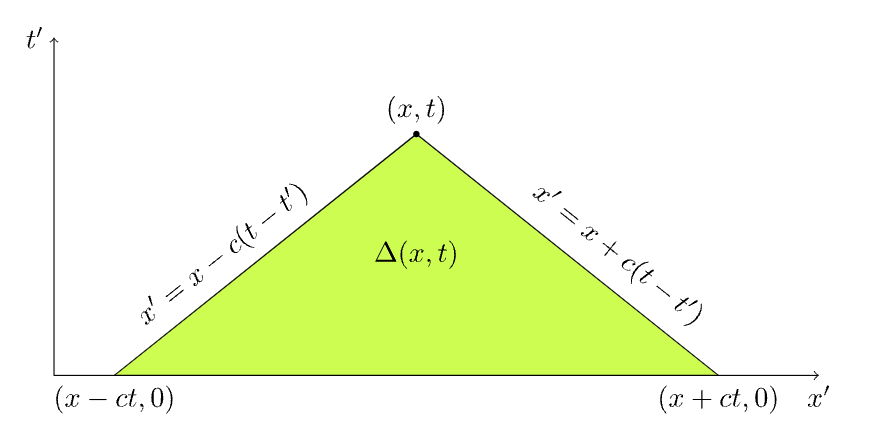
\includegraphics[width=12cm]{lightCone}
%   \caption{light cone and reverse light cone}
% \end{figure}

Notice that given d'Alembert's formula, the solution $u(t,x)$ given above depnds on the initial data $(f(x), g(x))$ only
for values $x'$ that is inside the backwards light cone, or more precisely the interior of the light cone with boundary
defined by the set above and the line $\{t = 0\}$:

PICTURE HERE

Thus, we say such a solution satisfies the principle of \emph{finite propagation speed}. Thus, if $f,g$ have compact
support within some interval $[-R. R]$,
\[
	\supp(u(t,x)) \sse [-R-|t|, R+|t|]
\]
as seen in figure BOOK IMAGE. if we consider the slope of the above to be $c$ (notice that $c= 1$, then the information
given by the initial data in the interval $[-R, R]$ does not travel faster then $c =1$, and so at tiem $t > 0$, the
information has not propogated further than $[-(R+t), (R+t)]$. This property is called \emph{Huygen's principle}, and
will appear often when we talk about solutions to wave equations.

(A word on the strong Huygen priniple)

\section{Duhamel's Principle}

We next look into the \emph{inhomogeneous} 1d wave equation:
\begin{equation}\label{eq:duhamelsPrinciple}
	\partial_t^2 u - \partial_x^2 u = h(t,x)
\end{equation}
with initial data
\[
	u(0,x) = f(x),\quad\partial_t u(0,x) = g(x),\quad h(t,x)\in C^2
\]
If we have $h(t,x) = 0$, then we can find a solution $u_1(t,x)$ using d'Alembert's formula, and if $f = g = 0$, it is
easy to get another [linear] solution $u_2(t,x)$, even if $h(t,x)$ is nonzero (as we'll explore momentarily). Thus, since
equation~(\ref{eq:duhamelsPrinciple}) is a linear equation,  we get a solution $u(t,x) = u_1(t,x) + u_2(t,x)$, gives the general solution! It remains to show how we can find $u_2$,
which will be used using \emph{Duhamel's principle}.

Start by solving the ``standard form'' of the IVP, namely with:
\[
	f = h = 0 \qquad \text{and} \qquad  g = h
\]
This comes from interpreting the $h$ function as giving a new ``force'' on the surface (in this 1-dimensional
case, string) which change the velocity, hence why $g = h$. Using d'Alembert's formula\footnote{you can veirfy
through
\href{https://math.stackexchange.com/questions/2509460/non-homogeneous-1-dimensional-wave-equation-with-arbitrary-initial-boundary-cond}{this
link}}, we get:
\[
	W_t(g, x) = u(t,x) = \int_{x-t}^{x+t}g(s)ds
\]
where we'll call $W_t(g, x)$, or just $W(t)$ the \emph{propagation operator} or \emph{solution operator}. Using this
operator, we can show that the general solution is in fact:

\[
	u(t,x)  = \partial_t(W_t(f, x)) = W_t(g, x)
\]
We simply verify that this satisfies the initial conditions. For $u(0,x)$:
\[
	u(0,x) = \partial_t(W_0(f, x)) + W_0(g, x) = f(x) + 0
\]
\[
	\partial_t u(0,x) = \partial_t\left(\partial_t(W_0(f, x))\right) + \partial_t(W_0(g, x)) = \nabla W_0(f, x) + g(x)
	= 0 + g(x)
\]
Now that we expressed the d'Alembert's solution when the IVP is in standard form, we will use this to show how to solve
the inhomogenous case. Letting $h \ne 0$, we'll show that:
\[
	u_2(t,x) = \int_0^t W(t-s)(h(s,\cdot))(x)ds
\]
Indeed, verifying directly that $u_2(t,x)$ satisfies the IVP:
\begin{align*}
	u_2(t,x) &= 0\\
	\partial_t u_2(t,x) &= \partial_t \left.\int_0^t W(t-s)(h(s,\cdot))(x)ds\right|_{t=0} = W(0)(h(t, \cdot))(x) = 0\\
		\partial_t^2 u_2(t,x) &= \int_0^t \partial_t^2W(t-s)(h(s, \cdot))(x)ds
		+ \partial_t\left(W(0)(h(t,\cdot))(x)\right)\\
		&= \nabla u_2(t,x) + h(t,x)
\end{align*}

Combining the result to get $u = u_1 + u_2$ and decomposing $W(t)(g)(x)$, we get:
\begin{align*}
	u(t,x) &= u_1(t,x) + u_2(t,x)\\
		   &= \frac{1}{2}\left(f(t+x) + f(x-t)\right) + \frac{1}{2} \int_{x-t}^{x+t} g(x')dx'\\
		   &\quad \frac{1}{2}\int_0^t \int_{x -(t-s)}^{x +(t-s)} h(s,x')dx'ds
\end{align*}

The double integral in the above takes into account the component $u_2(t,x)$ of the solutions over the backwards
light cone
\begin{figure}[H]
  \centering
  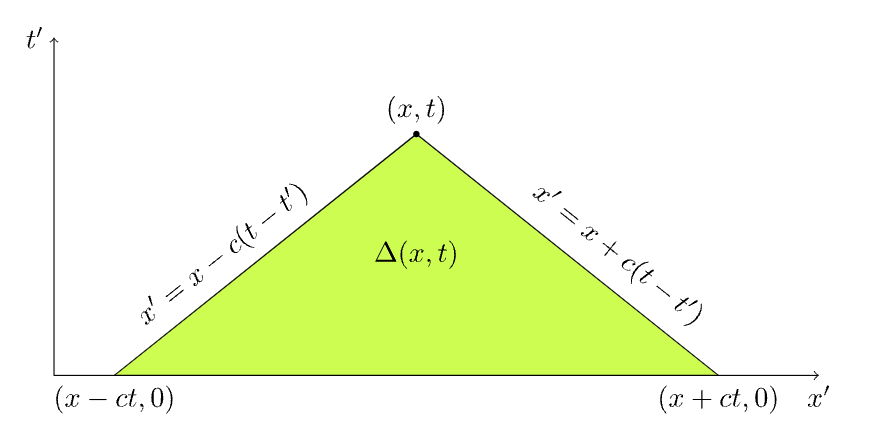
\includegraphics[width=7cm]{./lightCone}
  \caption{Light cone }
  \label{fig:lightConeRepresentation}
\end{figure}

\subsection{Boundary Problems}

Many times, a wave equation must also specify a boundary condition, thus we need to consider an \emph{initial boundary
problem}, or \emph{IBP} for short. An example of a boundary problem would be :
\[
	u(t,0) = 0
\]
which is known as the \emph{Dirchelet condition}, and
\[
	\partial_x u(t,0)  =0
\]
which is known as the \emph{Neumann condition}. We will start by solving wave equations with the Dirchelet condition.
We will take advantage of the fact that odd functions ($h(-x) = -h(x)$) that are continuous $x = 0$ must satisfy $h(0)
= 0$. Let's assuem the sapcial domain is only $\R_{\ge 0}$, so that the inital values $f(x), g(x)$ are only definedon
$\R_{\ge 0}$. Naturally, to be compatible with the IBP, we need that $f(0) = g(0) = 0$. We first define extension of
$f,g$ onto all of $\R$ by taking $f(-x) = -f(x)$, $g(-x) = -g(x)$. Using d'Alembert formula, we get the solution to the
cauchy problem:
\[
	u(t,x) = \frac{1}{2} \left( f(x+t) - f(x-t)\right) + \frac{1}{2}\int_{x-t}^{x+t} g(x')dx'
\]
Clearly, this expression is an odd fucntion with respect to $x$, since $f$ and $g$ are odd. Note that for any $x > t$,
this expression only involves the arguments of $f,g$ for positive $x$; however, for $x < t$, the expression involves
negative argument even though $x > 0$. To remedy this we use the fact that he extended $f,g$ are odd to rewrite the
expression as:
\[
	u(t,x) = \frac{1}{2} \left( f(t+x) - f(t-x)\right) + \frac{1}{2}\int_{t-x}^{t+x} g(x')dx'
\]
Thus, this solution is only dependnt upon $(f(x), g(x))$, $x > 0$. Due to the odd extension, the result looks like this
acccross time:
% \begin{figure}[H]
%   \centering
%   \includegraphics[width=12cm]{methodOfImages}
% \end{figure}

(Then there is solving the Neumann condition, which since we are taking the derivative will end up being the same type
of extension except it is an even extension instead of an odd one)

\begin{example}{Wave Equation Solutions}{waveEquationSolutions}
	\begin{enumerate}
		\item Consider:
			\[
				\begin{cases}
					u_{tt} - 9u_{xx} = 0 & -\infty < t < \infty,\ x > -t\\
					u|_{t=0} = 4\cos9(x) & x > 0\\
					u_t|_{t=0} = -2\cos(3x) & x > 0\\
					u|_{x=-t} = u_x|_{x=-t} = 0 & 0 < t < \infty
				\end{cases}
			\]
			Starting with the general solution, we get:
			\[
				u(x,t) = \phi(x+3t) + \psi(x-3t)
			\]
			With the IVP, we get:
			\begin{align*}
				\phi(x) + \psi(x) &= 4\cos(x) & x > 0\\
				\phi(x) - \psi(x) &= -6\cos(x) & x > 0\\
				\Rw \phi(x) = -\cos(x) &\qquad \psi(x) = 5\cos(x) & x > 0
			\end{align*}
			Hence the solution for this IVP with the right boundaries is:
			\[
				u(x,t) = -\cos(x+3t) + 5\cos(x-3t) \qquad x > 3|t|
			\]
			Now, for the boundary condition, we return to the original general solution and impose the
			boundary condition:
			\[
				u(x,t) = \phi(x+3t) + \psi(x-3t) \qquad u|_{x=-t} = u_x|_{x=-t} = 0 \qquad 0 < t < \infty
			\]
			plugging in ,we get:
			\[
				\phi'(2t) = \psi'(-4t) = 0
			\]
			For $t > 0$, we have $\phi$ defiend, so:
			\[
				\sin(2t) + \psi'(4t) = 0 \Rw \psi'(x) = \sin(x/2) \ \Rw\ \psi(x) = -2\cos(x/2) + C
			\]
			Hence for $t > 0$, $-t < x < 3t$, we get:
			\[
				u(x,t) = -\cos(x+3t) -2\cos((x-3t)/2) + 7
			\]
			Doing the same for $t < 0$, where instead $\psi$ is defined we get:
			\[
				u(x,t) = \frac{5}{2}\cos(2x) - \frac{7}{2} +5\cos(x-3t)
			\]
			The solution boundaries looks like:
			\begin{figure}[H]
			  \centering
			  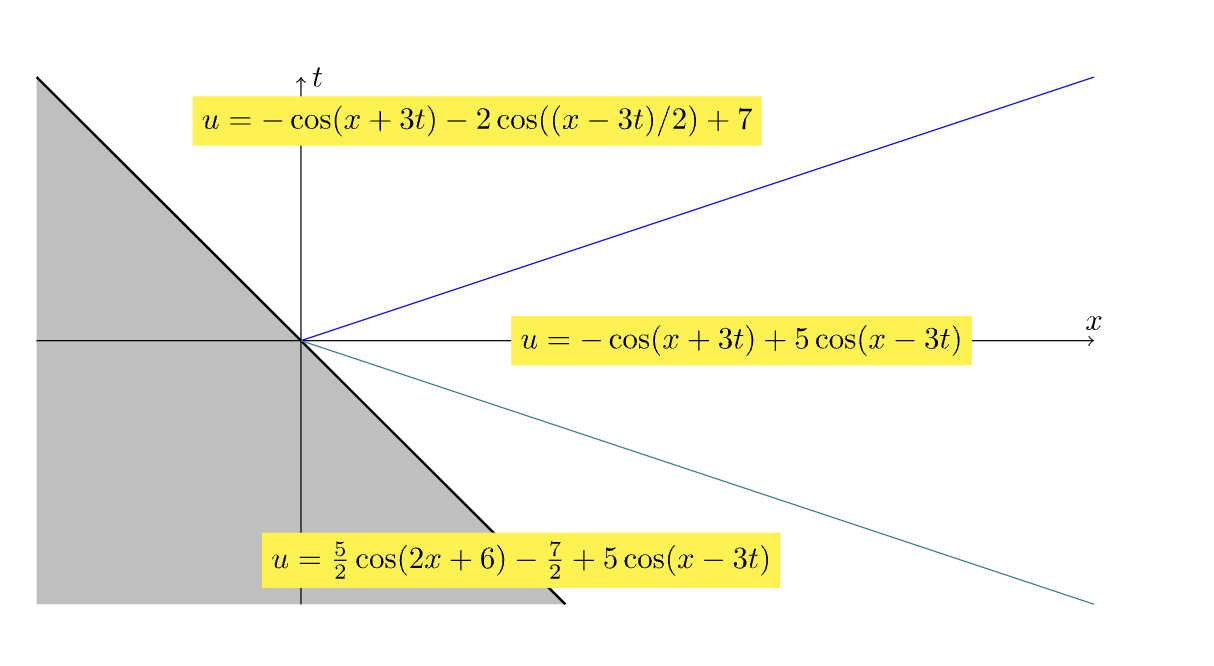
\includegraphics[width=7cm]{./solutionZone}
			  \caption{Where all the solutions are defined}
			  \label{fig:solutionZoneOfExample}
			\end{figure}
	\end{enumerate}
\end{example}

This is also a nice visual: \href{https://www.math.toronto.edu/ivrii/PDE-textbook/Chapter2/S2.6.V-A.html}{3 reflection types}.

\subsection{Separation of Variables}

Let:
\[
	 \partial_t^2 -  \partial_x^2 u  =0 \qquad x \in (0, 2\pi)
\]
with Dirichlet boundary conditions:
\[
	u(t,0) = 0 = u(t, 2\pi)
\]
we will seek a special solution in the form of the product $u(t,x) = v(t)w(x)$ (i.e. the relation between the time and
space variables can be seperated to ``independent'' function which interact via multiplication) so that:
\[
	 \partial_t^2 v w = v  \partial_x^2u
\]
Assuming the measure of points where $v,w = 0$ is zero, dividing both sides by $vw$, we get that a.e.:
\[
	 \frac{\partial_t^2 v}{v} =  \frac{  \partial_x^2 w }{w}
\]
Since the left hand side only dependts on $t$ while the right hand side only depends on $t$, the value of this equation
is necessarily a constant:
\[
	 \frac{\partial_t^2 v}{v} =  \frac{  \partial_x^2 w }{w} = \lambda
\]
This makes the problem into 2 ODE's: an \emph{evolution problem} for $v(t)$ in order to satisfy the initial conditions,
and an eigenvalue problem for an ODE for $w(x)$ so that the solution satisfie sthe boundary condtiions. The eigenvalue
probelm is for the pari $(w(x), \lambda)$, wher the function $w(x)$ satisfie the Dirichlet boundary conditions on $x \in
(0, 2\pi)$:
\[
	 \partial_x^2 w = \lambda w \qquad w(0) = 0 = w(2\pi)
\]
Given an eigenfunctio nand an eiganvalue from this problem, the evolution equation for $v$ is:
\[
	\frac{d^2}{dt^2}v = \lambda v
\]
with initia ldat a $v(0) = a$, $\dot v(0) = b$ that has to be specified. The eigenvalue problem has a countable number
of solutions, which are of the form:
\[
	w_k(x) =  \frac{1}{\sqrt{\pi}} \sin\left( \frac{1}{2}kx\right) \qquad \lambda_k = \frac{-k^2}{4},\ k \in \N_{>0}
\]
Thus, we can choose countably many constants $(a_k, b_k)$, $k \in \N_{>0}$ such that
\[
	v_k(t) = a_k\cos(w_k t) + b_k \frac{}{\sin(w_kt)}{w_k}
\]
with temporal fequencies $w_k = \sqrt{-\lambda_k} = \frac{1}{2}k$. Combining these give us the general solution:

\begin{thm}{General Solution To Seperation Of Variables}{generalSolutionToSeperationVariables}
	The genral solution of the initial-boundary value problem given at the beginning of this section is a lienar
	super position of these special solutiosn:
	\[
		u(t,x) = \sum_{k=1}^\infty \left( a_k\cos(w_k t) + b_k \frac{\sin(w_k
		t)}{w_k}\right)\frac{1}{\sqrt{\pi}}\sin\left( \frac{1}{2} kx\right)
	\]
	where the initail data is specified by:
	\[
		u(0,x) = f(x) = \sum_{k=1}^\infty a_k \frac{1}{\sqrt{\pi}} \sin\left( \frac{1}{2} kx\right) = \sum_{k=1}^\infty
		a_kw_k(x)
	\]
	and
	\[
		 \partial_t u(0,x) = g(x) = \sum_{k=1}^\infty b_k \frac{1}{\sqrt{\pi}} \sin\left( \frac{1}{2} kx\right) = \sum_{k=1}^\infty
		a_kw_k(x)
	\]
	Furthermore, the sine series used to describe $f(x), g(x)$ is compelte as an orthonormal basis for the Hilbert
	space $L^2(0, 2\pi)$; thus any initial $f(x), g(x) \in L^2$ can be represented by their Fourier sine series
	cofefficeints $(a_k, b_k)_{k \in ]N}$ giving rise to a solution $u(t,x)$.
\end{thm}

\begin{Proof}
	Just take everything we talked about earlier. For the $L^2$ basis, recall 457 and 357.
\end{Proof}

To Calculate the coefficeints, we do the usual trick in Hilbert spaces given an orthonormal basis, recalling that the
inner prodcut is:
\[
	\langle f,g\rangle = \int_{0}^{2\pi} f(x) \oln{g}(x)dx
\]

(Comments on how it applies to quantum mechanics and music here)

\section{Wave Equation in Higher Dimensions}

we now study equations of the form:
\[
	 \partial_t^2 u - \nabla u = 0
\]
where $u \in \R^{1+n}$ and $\nabla u = \sum_{i=1}^n \frac{\partial^2 u}{\partial x_i^2}$. This is often represented as:
\[
	\square u = 0
\]
\subsection{Fourier Series}


We first solve this using Fourier series. Assuming $f,g \in S$ is in the Schwartz class, we can take the Fourier
Transform and get:
\[
	\partial_t^2 \hat{u}(t, \xi) + |\xi|^2\hat{u}(t, \xi) = 0
\]
making this into an ODE. Solutions of this ODE are composed of linear combinations of $e^{\pm i |\xi| t}$. Takiung into
account that $\hat{u}(0,. \xi) = \hat{f}(\xi)$ and $\partial_t \hat{u}(0, \xi) = \hat{g}(\xi)$, we get the expression:
\[
	\hat{u}(t, \xi) = \cos(|\xi|t) \hat{f}(\xi) + \frac{\sin(|\xi|t)}{|\xi|}\hat{g}(\xi)
\]
And so the inverse fourier transform gives the solution:
\[
	u(t,x) = \frac{1}{\sqrt{2\pi}^n} \int e^{i\xi x} \left(\cos(|\xi|t) \hat{f}(\xi)
		+ \frac{\sin(|\xi|t)l}{|\xi|}\hat{g}(\xi)\right)d\xi
\]
Thus, if $f,g$ are of Schwartz class, we get a solution. However, this is by observation not necessary, we only need
that:
\[
	\hat{f} (\xi), \frac{\hat{g}(\xi)}{|\xi|} \in L^2(\R_x^n)
\]
to have a solution. We will soon explore this when we find weak solutions.

%(a word on how energy is conserved)

(a word on Lorenz Transfomration's leaving the solution independent, this is a prelude to chapter~\ref{cha:globalSolWaveEq})

\subsection{Method of Spherical Means}

\begin{defn}{Spherical Mean}{sphericalMean}
	Given a function $g \in C(\R^n)$, it's \emph{spherical mean} centered about the point $x \in \R^n$ is
	\[
		M(h)(x,r) = \frac{1}{w_nr^{n-1}}\int_{|x-y| = r} h(y)dS_y
	\]
	that is, it is the average of $h(x)$ over the sphere $S^{n-1}$ centered at $x$ of radius $r$.
\end{defn}

the constant in front is the normalization term: $w_nr^{n-1}$ is the surface area of the sphere $S^{n-1}$ of radius $r$
of dimension $n$. When $n = 1$, the sphere mean of a function $f(x)$ is:
\[
	M(f)(x, r) = \frac{1}{2}(f(x+r) + f(x-r))
\]
which is the first term the d'Alembert formula. If we do a change of variables in the equation in the definition to $y
\mapsto x + r\xi$, where $\xi \in S_1(0)$, there is another expression for the spherical mean:
\begin{equation}\label{eq:sphereMeanReDone}
	M(h)(x,r) = \frac{1}{w_n} \int_{|\xi| = 1}h(x + r\xi)dS_{\xi}
\end{equation}
Though we define if for $r \ge 0$, it is easy to see that equation~\ref{eq:sphereMeanReDone} shows that this function is even in $r$:
\[
	M(h)(x,-r) = M(h)(x,r)
\]

\begin{lem}{Darboux Equation}{darbouxEquation}
	Given $h \in C^2(\R^n)$,
	\[
		\triangle_x M(h)(x,r) = (\partial_r^2 + \frac{n-1}{r}  \partial_R)M(h)(x,r)
	\]
	a formula that realtes the Laplace operator of $M(h)$ in the $n$-dimensional $x$-variables to an operator involving
	only tone-dimeniwdimensional $r$ derivatives.
\end{lem}

\begin{Proof}
	This follows form computations using multivariable calculus. First, take one derivative:
	\begin{align*}
		\partial_r M(h)(x,r) &= \frac{1}{w_n} int_{|\xi| = 1} \partial_r h(x + r\xi)dS_{\xi}\\
							 &= \frac{1}{w_n}\int_{|\xi| = 1} \sum_{j=1}^n  \partial_{x_j}h(x + r\xi)\xi_j dS_{\xi}
	\end{align*}
	Notice that $\sum_{j=1}^n \partial_{x_j}h(x + r\xi)\xi_j = \nabla h\cdot N$,the outwards noraml derivative of $h$ on
	the unit sphere. Thus, we use Gren's theorem and continue:
	\begin{align*}
	 \frac{1}{w_n}\int_{|\xi| = 1} \sum_{j=1}^n  \partial_{x_j}h(x + r\xi)\xi_j dS_{\xi}
	 &= \frac{1}{w_n}\int_{|\xi| < 1} r\triangle_x h(x + r\xi)d\xi\\
	 &= \frac{1}{w_nr^{n-1}} \triangle_x \int_{|x-y| < r} h(y)dy\\
	 &= \frac{1}{w_nr^{n-1}} \triangle_x \left(\int_0^r\int_{|x-y|=\rho} h(y)dS_yd\rho\right)\\
	 &= \frac{1}{r^{n-1}} \triangle_x \left(\int_0^r\rho^{n-1}M(h)(x,\rho)d\rho\right)\\
	\end{align*}
	the next second is to take a second derivagie after multiplying through by $r^{n-1}$:
	\begin{align*}
		\partial_r\left(r^{n-1}  \partial_r M(h)(x,r)\right) &=  \partial_r \left(\triangle_x \int_0^r
		\rho^{n-1}M(h)(x,\rho)d\rho\right)\\
	&= \triangle_x\left(r^{n-1}M(h)(x,r)\right)
	\end{align*}
	Thus:
	\begin{align*}
		\triangle_x M(h)(x,r) &= \frac{1}{r^{n-1}}  \partial_r \left(r^{n-1}  \partial_r M(h)(x,r)\right)\\
		&= \left(  \partial_r^2 + \frac{n-1}{r}  \partial_r\right) M(h)(x,r)
	\end{align*}
	as we sought to show.
\end{Proof}

A couple of analysis facts worth reminding ourselve:

\begin{prop}{Analysis Facts}{analysisFacts}
	\begin{enumerate}
		\item For $h(x) \in C(\R^n)$, the value of $h(x)$ at any $x \in \R^n$ can be recovered from tis spherical mean:
			\[
				h(x) = \lim_{r \rw 0} M(h)(x,r) = M(h)(x,0)
			\]
			For $h(x) \in C^2(\R^n)$,
			\[
				\partial_r M(h)(x,0) = \lim_{r \rw 0} \frac{r}{w_n} \int_{|\xi| < 1} h(x + r\xi)d\xi = 0
			\]
	\end{enumerate}
\end{prop}

The first point will allow us to recoer the solution to wave equations posed in terms of the spherical mean ,while the
other will help in computaion.

\begin{Proof}
	See Folland chapter 3 section 4 to outline how to get this result, or your MAT457 notes
\end{Proof}

We can now use the spherical means formula to find solutions to the wave equations, in particular solutions that are not
as strong as being of Schwartz class. Next section, we will show how to find even weaker solutions.  Firs,t suppose that
$u(t,x)$ is a solution of the Cauch yproblem for the question equaiton. Then its spherical mean $M(u)(t,x,r)$ can be
defiend from the equation for the spherical means, and it satisfies an auxiliary equation in the reduced space-time
variables $(t,r) \in \R^2$. Specificaly, define:
\[
	M(u)(t,x,r) = \frac{1}{w_n} \int_{|\xi| =1} u(t, x + r\xi) dS_\xi
\]
Taking time derivatves and using the fact that $u(t,x)$ is a solution of the wave equation, we obtain:
\begin{align*}
	\partial_t^2 M(u)(t,x,r) &= \frac{1}{w_n} \int_{|\xi| =1}  \partial_t^2 u(t,x + r\xi) dS_\xi\\
							 &= \frac{1}{w_n} \int_{|\xi| = 1} \triangle_x u(t, x + r\xi) dS_\xi\\
							 &= \triangle_x M(u)(t,x,r)
\end{align*}
Now using the Darbous equation, we get:
\begin{equation}\label{eq:sphereMeansModified}
  \partial_t^2 M(u)(t,x,r) = \left(  \partial_r^2 + \frac{n-1}{r}  \partial_r\right) M(u)(t,x,r)
\end{equation}
a PDE in the two variables $(t,r) \in \R^2$. This is known as the \emph{Euler-Poisson-Darboux} equation.

\subsection{Spherical Mean in 3 Dimension}

We now show how to find solutiosn given the spherical Equation~(\ref{eq:sphereMeansModified}) is normally posed as an
IVP:

\begin{align*}
	 \partial_t^2 M(u)(t,x,r) &= \left(  \partial_r^2 + \frac{n-1}{r}  \partial_r \right) M(u)(t,x,r)\\
	 M(u)(0,x,r) &= M(f)(x,r)\\
	  \partial_t M(u)(0,x,r) &= M(g)(x,r)
\end{align*}

The solution of this will vary quite a bit on the dimension we choose. The case of $n =3$ is the simplest, and so we
start with it. First, we do the substituion $M(u)(t,x,r) \mapsto rM(u)(t,x,r)$, giving:
\[
	 \partial_t^2 \left(rM(u)(t,x,r)\right) = r\left(  \partial_r^2 + \frac{2}{r}  \partial_r \right) M(u)(t,x,r)
	 =   \partial_r^2 \left( rM(u)(t,x,r)\right)
\]
Thus, the function $v(t,r) = rM(u)(t,x,r)$ is a solution of the wave equation in one dimension, and the variable $x$ is
relegated to the role of a parameter. The solution is ginve by d'Alembert formula
\begin{align*}
	v(t,r) &= rM(u)(t,x,r)\\
	&= \frac{1}{2} \left( (r+t)M(f)(x, r+t) + (r-t)M(f)(x, r-t)\right)\\
	&\quad + \frac{1}{2} \int_{r-t}^{r+t} \rho M(g)(x,\rho) d\rho
\end{align*}

Since $M(f)(x,r)$ and $M(g)(x,r)$ are even functions under $r \mapsto -r$, the n$rM(f)(x,r)$ and $rM(g)(x,r)$ are odd;
therefore we may re-write the above expression, dividng through by $r$:
\begin{align*}
	M(u)(t,x,r) &= \frac{1}{2r} \left( (r+t)M(f)(x, r+t) + (r-t)M(f)(x, r-t)\right)\\
	&\quad + \frac{1}{2r} \int_{t-r}^{t+r} \rho M(g)(x,\rho) d\rho
\end{align*}
Note that we used the fact that $\int_{t-r}^{r-t} \rho M(g)(x,\rho)d\rho - 0$,  which holds since $rM(g)(x,r)$ is odd.
Taking the limit as $r \rw 0$ and using proposition~\ref{pr:analysisFacts}, we see that we recover
a representation
for the solution $u(t,x)$.


\begin{thm}{Kirchhoff's Formula}{kirchhoffFormula}
	When $n = 3$, the solution to the wave equation is given by the expression
	\begin{equation}\label{eq:kirchhoffsFormula}
	  u(t,x) =  \partial_t \left(tM(f)(x,t)\right) + tM(g)(x,t)
	\end{equation}
	which is well defined as long as $f(x) \in C^1(\R^3)$ and $g(x) \in C(\R^3)$
\end{thm}

\begin{Proof}
	Piece together all that was put above
\end{Proof}

Note that in terms of pointwise regularity, the solution is genreally less smooth than the initial data, for the
Kirchhoff formula depends upon the derivativge of $f(x)$. In particular, carrying out the differentiation in
equation~(\ref{eq:kirchhoffsFormula}), we obtain
\[
	u(t,x) = \frac{1}{4\pi t^2}\int_{|x-y| = t} \left(tg(y) = f(y) + t\nabla f(y)\cdot \frac{x-y}{|x-y|}\right) dS_y
\]
\begin{cor}{Solution Space}{solutionSp}
	Givien initial data $g(x) \in C^2(\R^3)$ and $f(x) \in C^3(\R^3)$, the spherical means solutions given in
	equation~(\ref{eq:kirchhoffsFormula}) is a solution $u(t,x) \in C^2(\R_t^1 \times \R_x^3)$
\end{cor}

\begin{Proof}
	Immediate.
\end{Proof}

(comment on loss of differentiability, and how this doesn't happen in Sobelev space)

\subsection{Spherical Means for odd Dimension}
Let's first recall the Euler-Poisson Daboux equation for the $n$-dimensional wave equation with IVP:


\begin{align*}
	 \partial_t^2 M(u)(t,x,r) &= \left(  \partial_r^2 + \frac{n-1}{r}  \partial_r \right) M(u)(t,x,r)\\
	 M(u)(0,x,r) &= M(f)(x,r)\\
	  \partial_t M(u)(0,x,r) &= M(g)(x,r)
\end{align*}

The goal is to have an algebraic reduction of the wave equation to two dimensions in the varaibvles $(t,r)$. This is
carrid out in the odd-dimenisonal case as follows:

\begin{lem}{Useful Relations}{usefulRelation}
	Suppose that $k \ge 1$ is an integer and that $h = h(r) \in C^{k+1}(R_+^1)$. Then:
	\begin{align*}
		\partial_r^2 \left( \frac{1}{r}  \partial_r \right)^{k-1} \left( r^{2k-1} h \right) &= \left(  \frac{1}{r}
		\partial_r \right)^k  \left( r^{2k}  \partial_r h \right)\\
		\left(  \frac{1}{r}  \partial_r \right)^{k-1} \left( r^{2k-1} h \right) = \sum_{j=0}^{k-1} \beta_j^k r^{j+1}
		\partial_r^jh
	\end{align*}
	with the combinatorial coefficients being $\beta_0^k = 1\cdot 3\cdot ... \cdot (2k-1) := (2k-1)!!$.
\end{lem}

\begin{Proof}
	Simply do an argument by induction
\end{Proof}

The ruslt is now useful since we can set $n = 2k + 1$ and take:
\[
	v(t,x,r) :=  \left(  \frac{1}{r}  \partial_r \right)^{k-1} \left( r^{2k-1} M(u) \right) (t,x,r)
\]
For a give solution $u(t,x)$ of the wave equation. Then using the identies from corrollary~\ref{lm:usefulRelation}
\begin{align*}
	\partial_r^2 v &=	  \partial_r^2 \left(  \frac{1}{r}  \partial_r \right)^{k-1} \left( r^{2k-1} M(u) \right)\\
	&= \frac{1}{r}  \partial_r^k \left(  r^{2k}  \partial_r M(u) \right)\\
	&= \left( \frac{1}{r}  \partial_r \right)^{k-1}  \left( r^{2k-1}  \partial_r^2 M(u) + 2kr^{2k-2}  \partial_r M(u)
	\right)\\
	&=\left( \frac{1}{r}  \partial_r \right)^{k-1} \left( r^{2k-1} \left(  \partial_r^2 M(u) + \frac{2k}{r}  \partial_r M(u)\right) \right)\\
	&= \left( \frac{1}{r}  \partial_r \right)^{k-1} \left( r^{2k-1}  \partial_t^2 M(u) \right)\\
	&=  \partial_t^2 v(t,r)
\end{align*}

Thus, $v(t,x,r)$ is the quantity that satisfies the one-dimensional wave equation in the variables $(t,r)$, for which we
can applyh the d'Alembert formula:
\[
	v(t,x,r) = \frac{1}{2} \left(v(0,r+t) + v(0, r-t)\right) + \frac{1}{2} \int_{r-t}^{r+t}  \partial_t v(0,x,
	\rho)d\rho
\]
with initial data:
\begin{align*}
	v(0,x,r) &= \left(  \frac{1}{4}  \partial_r \right)^{k-1} \left( r^{2k-1} M(f) \right) (x,r)\\
	 \partial_tv(0,x,r) &= \left(  \frac{1}{4}  \partial_r \right)^{k-1} \left( r^{2k-1} M(g) \right) (x,r)\\
\end{align*}

Then we can recover the solution as a limit:
\begin{align*}
	u(t,x) &= \lim_{r \rw 0} M(u)(t,x,r) = \lim_{r \rw 0} \frac{v(t,x,r)}{\beta_0^kr}\\\\
		   &= \frac{1}{(n-2)!!} \left[  \partial_t \left(  \frac{1}{t}  \partial_t \right)^{(n-3)/2} \left( t^{n-2}
		   M(f)(t,x) \right) + \left(  \frac{1}{t}  \partial_t \right)^{(n-3)/2} \left(t^{n-2} M(g)(t,x)\right)\right]
\end{align*}

Piecing it all together:

\begin{thm}{Solution For Odd Dimension}{solutionForOdd}
	For $n$ odd, $f \in C^{(n-1)/2}(\R^n)$ and $g \in C^{(n-3/2}(\R^n)$, the solution formula given above gives
		a classical solution to the wave equation in $\R^n$
\end{thm}

\begin{Proof}
	piece the above together
\end{Proof}

It is intereting that we can quantify the possibler loss of smoothness of the solution voer the initial data, made claer
by the formula above the theorem. Indeed, the reduction process from $M(u)$ to $v$ involves $k-1 = (n-3)/2$ derivatives,
and the limit involve sone derivative; therefore in general the solution will be less regular than the initial data by
$k = (n-1)/2$ many derivatives.


\subsection{Huygen's Principle}

Just like in the one-dimenisonal case, the information of the wave equation only propagates finitely far. We will see
that the strong Huygen principle will hold for odd dimensions but not for even. In the follwoing, we will show it for $n
=3$:

\begin{thm}{Huygen's Principle And Strong Huygen's Principle}{huygenPrincipleAndStrongHuygenPrinciple}
	Consider solutions to the wave equatio nfor $x \in \R^3$ and assume that the Cauchy data $f(x)$ and $g(x)$ are
	compactlysupported such that $\supp(f) \cup \supp(g) \sse B_R(0)$. Then:
	\begin{enumerate}
		\item \bf{(Huygen's principle)}: The solution $u(t,x)$ has its support within the bounded region $B_{R + |t|}(0)$:
			\[
				\supp(u(t,\cdot)) \sse B_{R + |t|}(0)
			\]
		\item \bf{(Strong Huygen's principle)}: Additionally, for $|t| > R$, for any space-time point $(t,x)$ in the region
			inside the light cones given by $\set{(t,x)}{ |x| \le |t| - R}$, again the solution vainshes; $u(t,x) = 0$
	\end{enumerate}
\end{thm}

\begin{Proof}
	\begin{enumerate}
		\item The result follows from kirchhoff's Formula
		\item When $|t| > R$, and $|x| < |t| - R$, again the backwards light cone emanating from the point $(t,x)$ does
			not intersect the support of the initial dta, in this case because the sphere $\set{y}{ |x=y| = |t|}$ is too
			big and has passed outside of $B_R(0)$.

			This proof is geometric, only depending upon the fact that the solution is represented as a spherical mean.
			Therefore the result holds for solutions of the wave equation in arbitrary odd dimension, as shown in the
			equation above theorem~\ref{th:solutionForOdd}.
	\end{enumerate}
\end{Proof}

(something slightly stronger is in fact true. p. 133 of ``A Course on PDEs'' by Walter Craig.

\subsection{Duhamel's Principle in Higher Dimensions}

here

\chapter{Weak Solutions and Distributions}\label{cha:distrib}

We know deal with the case where solutions can be ``weaker''. As we saw, d'Alembert formula works perfectly well if $f,g
\in L_{\text{loc}}^1(\R)$. However, the initial conditions \emph{require} that $f,g$ be differentiable (afterall, they
are slices of the function $u(t,x)$ and $  \partial_t u(t,x)$, which must be at least twice and once differentiable
respectively). So is there some way to circumnavigate this? The content of the first section of this chapater covers precisely
this. In the next section, we shall generlize the results and define a whole new object that will allow us to grealy
broaden our notion of function that will allow us to differentiate function that are simply locally itnegrable!

Let's start with the usual solution $u \in C^2$ on a time strip:
\[
	S_T = [0, T]\times \R^n
\]
and assume that:
\[
	\square u = F\qquad u|_{t=0} = f \qquad  \partial_t u|_{t=0} = g
\]
We are going to use the idea of a test function $\phi$. If you want to think of it in a Folland way, $\phi \in
C_c^\infty(S_T)$, and we are defining a functional on $C_c^\infty(S_T)$ taking $\phi \mapsto \int \square u \phi
d(x,t)$. We will take advantage of integration by parts to get the following:
\begin{align*}
	\int_{S_T} F\phi dtdx &= \int_{S_T}(\square u)\phi\, \textrm{d}t\textrm{d}x\\
  &= \int_{\R^n} \left( - \int_{0}^{T}  \partial_t u  \partial_t \phi\,\textrm{d}t - g(x)\phi(0, x) \right)\,\textrm{d}x
  - \int_{S_T} u\triangle \phi\, \textrm{d}t \textrm{d}x\\
  &= \int_{S_T} u\square \phi \textrm{d}t \textrm{d}x + \int_{\R^n} f(x)  \partial_t \phi(0,x)\, \textrm{d}x
  - \int_{\R^n} g(x) \phi(0,x) \textrm{d}x
\end{align*}
Which leads us to the following definition:
\begin{defn}{Weak Solution}{weakSolution}
	Let $f,g \in L_{\text{loc}}^1(\R^n)$ and $F \in L_{\text{loc}}(S_T)$. We say $u \in L_{\text{loc}}(S_T)$ is
	a \emph{weak solution} of the wave equation if:
	\begin{equation}\label{eq:weakSolEq}
	  \int_{S_T}(\square u)\phi\, \textrm{d}t\textrm{d}x = \int_{S_T} u\square \phi \textrm{d}t \textrm{d}x - \int_{\R^n} f(x)  \partial_t \phi(0,x)\, \textrm{d}x
	  + \int_{\R^n} g(x) \phi(0,x) \textrm{d}x
	\end{equation}
	for all $\phi \in C_c^\infty$ supported in $(-\infty, T)\times \R^n$
\end{defn}

The next shows how this is indeed a generization:

\begin{prop}{When Weak Solution Is Classical Solution}{WeakSolutoinIsClassicalSolution}
	A weak solution that belongs to $C^2(S_T)$ is a classical solution
\end{prop}

\begin{Proof}
	Taking equation~(\ref{eq:weakSolEq}),  we see first that:
	\[
		\int u\square \phi\, dtdx = \int F\phi\, dtdx
	\]
	and integratin by parts gives us that $\int u\square \phi = \int(\square u)\phi$. For the next part, recall that if
	$h \in L_{\text{loc}}^1$ and $\int h\phi = 0$ for all $\phi \in C_c^\infty$, then $h = 0$ almost everywhere. Thus
	since:
	\[
		\int (\square u - F)\phi dtdx = 0
	\]
	and $\phi$ was arbitrary, we conclude that $\square u = F$ on $S_T$ up to zero-measure.

	Next, we need to show that $u$ takes on the initial values of $f$ and $g$. Let's first show that:
	\[
		 \partial_t u(0, x) = g(x)
	 \]
	 First, the above equation is equivalent to:
	 \begin{equation}\label{eq:weakSolEquiv}
	   \int_{\R^n}  \partial_t u(0,x) \psi(x)dx = \int_{\R^n} g(x)\psi(x)dx \quad\text{for all $\psi \in C_c^\infty(\R^n)$}
	 \end{equation}
	 Fix any such $\psi$. we will do some clever manipulation to ``eliminate'' the integral. Let $a(t)$ be the smooth step function going from $1$ to zero smoothly:
	 \[
		 a(t) = \begin{cases}
			 1 &\text{for $0 \ge t$}\\
			 \text{smoooth} & \text{for $0 \le t \le 1$}\\
			 0 & \text{for $t \ge 1$}
		 \end{cases}
	 \]
	 Then $\theta_k(t) = a(kt)$ will squish the function so that it's closer and closer to being a step function.
	 Importantly for us, notice that $\theta_k$ has the following properties:
	 \[
		 \theta_k'(0) = 0\qquad \theta_k(t) = 0 \quad\text{for $t \ge 1/k$}
	 \]
	 Now, letting $\phi = \phi_k = \theta_k(t)\psi)$ from equation~(\ref{eq:weakSolEq}), then the right hand side of
	 equation~(\ref{eq:weakSolEq}) reads as (taking $k$ large enough so that $1/k < T$):
	 \begin{equation}\label{eq:fancySubstituionForWeakIsClassical}
	   \int_{\R^n} \left( \int_{0}^{1/k} F(t,x)(akt)\,\textrm{d}t \right)\psi(x)dx + \int_{\R^n} g(x)\psi(x)dx
	 \end{equation}
	 Since $F \in C(S_T)$ (recall $\square u = F$), the first term is $O(1/k)$ as $k \rw \infty$. Now, I claim that the
	 left hand side of equation~(\ref{eq:weakSolEq}) is equal to:
	 \begin{equation}\label{eq:claimForWeakIsClassical}
	   \int_{\R^n}  \partial_t u(0,x)\psi(x)\, dx + O(1/k)
	 \end{equation}
	 Notice that if (\ref{eq:fancySubstituionForWeakIsClassical}) equals to (\ref{eq:claimForWeakIsClassical}), then as
	 we take the limit as $k \rw \infty$, we get equation~(\ref{eq:weakSolEquiv}). To show this is the case, notice the
	 left hand side of (\ref{eq:weakSolEq}) is:
	 \[
		 \int_{S_T} u(t,x) \theta_k''(t)\psi(x)dtdx - \int_{\R^n} \left( \int_{0}^{1/k} u(t,x)a(kt)dt \right)\triangle
		 psi(x)dx
	 \]
	 The second term in the above is $O(1/k)$, and after integration by parts the first term becomes:
	 \[
		 -\int_{S_T}  \partial_tu(t,x) \theta_k'(t)\psi(x)dtdx
	 \]
	 (Note that there are no boundary terms since $\theta_k'(t) = 0$ for $t = T = 0$). Doing integration by parts
	 a second time, we get:
	 \[
		 \int_{\R^n} \left( \int_0^{1/k}  \partial_t^2 u(t,x) a(kt)dt \right)\psi(x)dx + \int_{\R^n}  \partial_t
		 u(0,x)\psi(x)dx
	 \]
	 where again the first term is $O(1/k)$, which proves the claim, and thus completes the proof
 \end{Proof}

 (exercise doing the same for showing that $u(0,x) = f(x)$. It proceeds like the proof above, but this time choosing
 $\theta_k(t) = \frac{1}{k} b(kt)$ where $b$ is some smooth compactly suported function such that $b(0) = 0$ and $b'(0)
 =1$, thus $\theta_k(0) = 0$ and $\theta_k'(0) = 1$ and the support shrinks to the origin as $k \rw \infty$ (see that
 the error term is not $O(1/k^2)$))

\begin{example}{Weak Solution}{weakSolutionEx}
	\begin{enumerate}
		\item I think putting some examples here is a good idea
	\end{enumerate}
\end{example}

\section{Distributions}


Distributions a generlization of functions that allow us to give more general solution than classical solutions,
similar to how we found a weak solution. Locally integrable functions will be distributions (in the
appropriate interpretation), but we'll see that there are general solution's that don't even fall under the notion of
``function''.

\subsection{Intuition}

For now, let $f \in L^p$. Then as we know, $(L^p)^* \cong L^q$ is an isometry where $1 \le p < \infty$. In particular,
we have that
\[
	g\mapsto \int fg
\]
is mapped to by $f$. Using the Lebesgue differentiation theorem, by
choosing $\phi_k = m(B_r)^{-1}\chi_{B_r}$, where $B_r$ is a ball of ardius $r$ around $x$, will allow us to recevoer the
value of $f(x)$ for a.e. $x$, as $\lim_{r \rw 0} \int f\phi_r$. In this way, we can think of $L^p$ as being embedded
into $(L^q)^*$ (since we really only care what happens a.e.).

Now, let us modify the above by letting $f$ be merely locally integrable (in $L_{\text{loc}}^1$), but $\phi \in
C_c^\infty$. Then it is clear that $\phi \mapsto \int f\phi$ is still a well-defined functional on $C_c^\infty$
,  and  the pointwise  values  of $ f$  can be  rcecoved  a.e. from it, by extending theroem ref: HERE (8.15 in
Folland). Unlike in the case for $L^p$ spaces, there are in fact \emph{many} linear functionals on $C_c^\infty$ that are
\emph{not} of the form $\phi \mapsto \int f\phi$. These, subject ot some mild continuity conditions we will soon
specify, will be our ``generlized functions''.



\subsection{Definitions}

We will first rapid-fire some important definitions to be up to speed with terminology. Recall that $C_c^\infty(E)$
where $E \sse \R^n$ is the set of all smooth functions whose support is compact and contained in $E$. If $U \sse \R^n$
is open, $C_c^\infty(U)$ is the union of space $C_c^\infty(K)$ where $K$ ranges oer all compact subsets of $U$. Each
$C_c^\infty(K)$ is a Fr\'echet space with the topology defined by the norms
\[
	\phi \mapsto \|  \partial^\alpha\|_u \qquad (\alpha \in \{0,1,2,...\}^n)
\]
Thus ,the sequence $\{\phi_i\}$ converges if and only if $  \partial^ \phi_i \rw  \partial^\alpha \phi$ uniformly for
all $\alpha$. The completness of $C_c^\infty(K)$ is shown through exercise $9$ in folland in section 5.1. With these, we
take the following definitions:
\begin{enumerate}
	\item  A sequence $\{\phi_i\}$ in $C_c^\infty(U)$ converges in $C_c^\infty$ to $\phi$ is $\{\phi_i\} \sse
		C_c^\infty(K)$ for some compact set $K \sse U$ and $\phi_i \rw \phi$ in the topology of $C_c^\infty(K)$, that
		is, $  \partial^\alpha \phi_i \rw  \partial^\alpha \phi$ uniformally for all $\alpha$
	\item If $X$ is a locally convex topologicla vector space and $T: C_c^\infty(U) \rw X$ is a linaer map, $T$ is
		\emph{continuous} if $T|_{C_c^\infty(K)}$ is continous for each compact $K \sse U$, that is, if $T(\phi_i) \rw
		T(\phi)$ whenever $\phi_i \rw \phi$ in $C_c^\infty(K)$ and $K \sse U$ is compact
	\item A linear map $T: C_c^\infty(U) \rw C_c^\infty(U')$ is \emph{continuous} if for each compact $K \sse U$, there
		is a compacty $K' \sse U'$ such that $T(C_c^\infty(K)) \sse C_c^\infty(K')$ and $T$ is continuous from
		$C_c^\infty(K)$ to $C_c^\infty(K')$
\end{enumerate}

With these, we will define a distribution:

\begin{defn}{Distribution}{distrib}
	A \emph{distribution} on $U$ is a continous lihear functional on $C_c^\infty(U)$. The space of all distributiosn on
	$U$ is denoted by $\CD'(U)$, and we set $\CD' = \CD'(\R^n)$. We impose the weak$^*$ topology on $\CD'(U)$, that is,
	the topology of pointwise converge on $C_c^\infty(U)$.
\end{defn}

A couple of remarks are in order: first, the $\CD'$ notation comes from the fact that Schwart'z used the notation of
$\CD$ for $C_c^\infty$ (probably because such functions are \emph{D}ifferentiable), and so $\CD'$ was the funcitonals on $C_c^\infty$. Next, there is a locally convex topology on
$C_c^\infty$ with respect to which sequential convergence in $C_c^\infty$ is given by the convergence defined earlier in
$C_c^\infty$, and the continuity of a linear map $T: C_c^\infty \rw X$ and $T: C_c^\infty \rw C_c^\infty$ is given by
the other two points. However, to define it is relatively complicated and doesn't contribute much to the current
exposition of distributions , and so will be ommited.

Before giving some examples of distributions, we will remind the reader how of how to check for continuity in a TVS:

\begin{prop}{Distribution Continuity Check}{distribContCheck}
	Let $u: C_c^\infty(U) \rw \R$ (or $\C$) be linear. Then $u \in \CD'(U)$ if and only if for every compact set $K \sse
	U$, there exists a $C_K > 0$ and $N_K \in\N$ such that
	\[
		\| \langle u, \phi\rangle\| \le C_k \sum_{\|\alpha\| \le N_K} \|  \partial^\alpha \phi\|_L^\infty
	\]
\end{prop}

\begin{Proof}
	Given the above equation, then it is easy to check  that if $\phi_i
	\rw \phi$, then $\langle u, \phi_i\rangle \rw \langle u, \phi\rangle$. (see chapter~\ref{cha:nonLinEq} for details)
\end{Proof}

\begin{example}{Distributions}{distribsEx}
	\begin{enumerate}
		\item For every $f \in L_{\text{loc}}^1(U)$, we can define a distribution on $U$< namely the funcitonal $\phi
			\rw \int f\phi$, and two functions define the same distributiosn precisely when they are equal a.e.
		\item Every Radon measure $\mu$ on $U$ defines a distributiosn $\phi \mapsto \int \phi d\mu$.
		\item If $x_0 \in U$ and $\alpha$ is a multi-index, the map $\phi \mapsto  \partial^\alpha(x_0)$ is
			a distribution that does not arise from a function; it arises from a measure $\mu$ prcisely when $\alpha
			= 0$, in which case $\mu$ is the point mass at $x_0$
		\end{enumerate}
\end{example}

As mentioned earlier, we often will associate the a function $f$ with the distribution it has, and even label the
distribution by $f$. For this reason, it might be confusing to write $f(\phi)$ to mean the distribution defined by $f$
taking in $\phi$, and so for historical reasons we use the notation $\langle f, \phi\rangle$.

Let's next establish some common notation:
\begin{enumerate}
	\item First, it is often enough that we will reflect function. Thus, if we put a tilde over a function, we mean:
		\[
			\tilde{\phi}(x) = \phi(-x)
		\]
	\item Second, the point-mass is a very common distribution, which we will denote by $\delta$:
		\[
			\langle \delta, \phi\rangle = \phi(0)
		\]
\end{enumerate}

As an example of the use of the detla funciton:

\begin{prop}{Convergence To Delta Function}{convergenceToDeltaFunction}
	Let $f \in L^1(\R^n)$ and $\int f = a$, and for $t > 0$, let $f_t(x) = t^{-n}f(t^{-1}x)$. Then$f_t \rw a\delta$ in
	$\CD'$ as $t \rw 0$
\end{prop}

\begin{Proof}
	If $\phi \in C_c^\infty$, by theroem 8.15, we have:
	\[
		\langle f_t, \phi\rangle = \int f_t\phi = f_t * \tilde{\phi}(0) \rw a\tilde{\phi}(0) = a\phi(0) = a\langle
		\delta, \phi\rangle
	\]
	completing the proof.
\end{Proof}

For equality of distributions, note that it makes to say that $F = G$ on an open set $V$ if and only if $\langle F,
\phi\rangle = \langle G,\phi\rangle$ for all $\phi \in C_c^\infty(V)$. If $F$ and $G$ are continuous functions, this will
imply they are pointwise equal, and if $F$ and $G$ are only locally integrable,this means they are equal a.e. on $V$.

Since a function in $C_c^\infty(V_1\cup V_2)$ need not be supported in either $V_1$ or $V_2$, it is not immediately
obvious that if $F = G$ on $V_1$ and on $V_2$ then $F = G$, then $F = G$ on $V_1\cup V_2$. However, this is the case:

\begin{prop}{Equality On Support}{equalityOnSupport}
	Let $\{V_\alpha\}$ be a collectio nof open subsets of $U$ and let $V = \bigcup_\alpha V_\alpha$. If $F,G \in
	\CD'(U)$ and $F = G$ on each $V_\alpha$, then $F = G$ on $V$
\end{prop}

\begin{Proof}
	Folland p. 284
\end{Proof}


As a consequence of proposition~\ref{pr:equalityOnSupport}, if $F \in \CD'(U)$, there is a maximal open subset $U$ on
which $F = 0$, namely the union of all open subset on which $F = 0$. Its compliment in $U$ is called the \emph{support}
of $F$. If it's compliment is compact, it is called the \emph{compact support}.

One of amazing facts about distributions is that even though they are not ``functions'', we will be able to do many
functional operations like diferentation, multiplication by a ``constant'', convolution, and translation!! To achieve
this, we need some theoretical build-up. Suppose $U$ and $V$ are open sets in $\R^n$ and $T$ is a liner map from some
subsapce $V$ of $L_{\loc}^1(U)$ into $L_{\loc}^1(V)$. Suppose that there is antoher linaer map $T':
C_c^\infty(V) \rw C_c^\infty(U)$ such that
\[
	\int (Tf)\phi = \int f(T'\phi) \qquad (f \in V,\ \phi \in C_c^\infty(V))
\]
suppose that $T'$ is continuous in the sense defined earlier. Then $T$ can be extended to a map from $\CD'(U)$ to
$\CD'(V)$, still dentoed by $T$, by:
\[
	\langle TF,\phi\rangle = \langle F, T'\phi\rangle \qquad (F \in \CD'(U),\ \phi \in C_c^\infty(V))
\]
The continuity of $T'$ guarantees that the original map $T$, as well as the extension to distributions, is continuous
with respect to the weak$^*$ topology on distributions, namely if $F_\alpha \rw F \in \CD'(U)$, then $Tf_1a \rw TF$ in
$\CD'(V)$. With this, we can define the following on distributions
\begin{enumerate}
	\item (Differentiation) Let $Tf =  \partial^\alpha f$, defined on $C^{|\alpha|}(U)$. If$\phi \in C_c^\infty(U)$,
		integration by parts gives $\int (  \partial^\alpha f )\phi = (-1)^{|\alpha|}\int f(  \partial^\alpha \phi )$;
		there are no boundary terms since $\phi$ has compact suppor.t. Henc $T' = (-1)^{|\alpha|}T|_{C_c^{\infty}(U)}$,
		and we can define the \emph{derivative} $  \partial^\alpha F \in \CD'(U)$ of any $F \in \CD'(U)$ by:
		\[
			\langle  \partial^\alpha F, \phi\rangle := (-1)^{|\alpha|}\langle F,  \partial^\alpha, \phi\rangle
		\]
		By this procedure, we can define the derivatives of arbirary locally integrabl funtions, even when they are not
		differentiable in the classical sense! We will give the derivative of certain locally integrable functions
		soon!!
	\item (multiplication by a smooth function, a ``scalar'') Let $\psi \in C^\infty(U)$ and define $Tf= \psi f$. Then
		evidently, $T' = T|_{C_c^\infty(U)}$, and so we can define $\psi F \in \CD'(U)$ for any $F \in \CD'(U)$ to be:
		\[
			\langle \psi F, \phi\rangle := \langle F, \psi\phi\rangle
		\]
	\item (Translation) Let $y \in \R^n$ and let $V = U + y = \set{x+y}{x \in U}$. Take $T = \tau_y$ (recall that
		$\tau_yf(x) = f(x-y)$). Via u-substituion, we get that $\int f(x-y)\phi(x)dx = \int f(x)\phi(x+y)dx$, and so $T'
		= \left.\tau_{-y}\right|_{C_c^\infty(U)}$. For a distribution $F \in \CD'(U)$, we define:
			\[
				\langle \tau_yF, \phi\rangle := \langle F, \tau_{-y}\phi\rangle
			\]
	\item (convolution with linear maps) Let $S$ be an invertible linear transformation from $\R^n$ to $\R^n$. Letting
		$V = S^{-1}(U)$ and $Tf = f\circ S$, Then $T'\phi = |\det(S)|^{-1} \phi \circ S^{-1}$ (by change of variables,
		see theorem ref:HERE).
		Thus, for $F \in \CD'(U)$, define:
		\[
			\langle F\circ S, \phi\rangle := |\det S|^{-1}\langle F, \phi \circ S^{-1}\rangle
		\]
	\item (convolution I) Let $\psi \in C_c^\infty$, and let
		\[
			V= \set{x}{x-y \in U\text{ for $y\in \supp(\psi)$ }}
		\]
		Note that $V$ is open but may be empty. If $f \in L_{\text{loc}}^1(U)$, we get that the integral:
		\[
			f* \psi(x) = \int f(x-y)\psi(y)dy = \int f(y)\psi(x-y)dy = \int f(\tau_x \tilde{\psi})
		\]
		is well-defined for all $x \in V$. Since we transfered over from $f$ to $\psi$, we can define for $F \in
		\CD'(U)$:
		\[
			F*\psi(x) = \langle F, \tau_x\tilde{\psi}\rangle
		\]
		Since $\tau_x \tilde{\psi} \rw \tau_{x_0} \tilde{\psi}$ as $x \rw x_0$, $F*\psi$ is a continuous function (in
		fact, $C^\infty$, as we'll show in a moment). A pertinent example of this is the following:
		\[
			\delta * \psi(x) = \langle \delta, \tau_x \tilde{\psi}\rangle = \tau_x \tilde{\psi(0)} = \psi(x)
		\]
		so $\delta$ is the multiplicative identity of convolution!
	\item (convolution II) Let $\psi, \tilde{\psi}$ and $V$ be like the last point. If $f \in L_{\text{loc}}^1(U)$ and
		$\phi \in C_c^\infty(U)$, then
		\[
			\int (f*\psi)\phi = \int\int f(y)\psi(x-y)\phi(y)dydx = \int f(\phi*\tilde{\psi})
		\]
		Thus $Tf = f*\psi$ maps $L_{\text{loc}}^1(U)$ to $L_{\text{loc}}^1(V)$ and $T'\phi = \phi* \tilde{\psi}$. Thus,
		we get:
		\[
			\langle F*\psi, \phi\rangle = \langle F, \phi*\tilde{\psi}\rangle
		\]
\end{enumerate}

(theorem on how the two convolutions are actually the same thing)

Next, we will show that smooth compact functions $C_c^\infty(U)$ are dense in $\CD'(U)$

\begin{lem}{Build-Up For Density}{maBuild-UpForDensity}
	Suppose that $\phi \in C_c^\infty, \psi C_c^\infty$ and $\int \psi = 1$, and let $\psi_t(x) = t^{-n}\psi(t^{-1}x)$.
	Then
	\begin{enumerate}
		\item Given any neighborhood $U$ of $\supp(\phi)$, we have $\supp(\phi* \psi_t) \sse U$ for $t$
		\item $\phi * \psi_t \rw \phi$ in $C_c^\infty$ as $t \rw 0$
	\end{enumerate}
\end{lem}

\begin{Proof}
	Folland p. 287
\end{Proof}


\begin{prop}{Density Of Smooth Compact Functions In Distributions}{densitySmoothCompFunctionsInDistribs}
	Let $U \sse \R^n$ be open. Then $C_c^\infty(U)$ is dense in $\CD'U)$ in the topology of $\CD'(U)$
\end{prop}

\begin{Proof}
	Folland p. 287
\end{Proof}

\subsection{More continuity properties}

Suppose
\[
	u_i \rw u \text{ in } \CD'(U) \qquad \phi_i \rw \phi \text{ in } C_c^\infty(U)
\]
Then is it true that:
\[
	\langle u_i, \phi_i\rangle \rw \langle u, \phi\rangle
\]
The answer is yes, though it is not immediate. First, using bilinearity, we can re-write the left hand side as the right
hand side in the following:
\[
	\langle u_i, \phi_i \rangle - \langle u,\phi \rangle = \langle u_i, \phi_i - \phi \rangle + \langle u_i - u, \phi\rangle
\]
Since we have that $u_i \rw u$, the second term on the right hand side certainly goes to zero. However, as $u_i$ varies,
it is not clear that the first term on the right hand side goes to zero. However, if the continuity estimate given in
proposition~\ref{pr:distribContCheck} would hold for all $u_i$ with some constant $C_k$ and $N_k$ (i.e.
\emph{independent} of $i$), then the first term would also converge to zero, since $\phi_i \rw \phi$. In fact, it turns
out that such estimates do indeed exist, which is very non-trivial since the convergence in $\CD'(U)$ has the topology
given by pointwise convergence! To show this, we requires some important build-up results:

\begin{thm}{Uniform Boundedness Principle}{uniformBoundednessPrinciple}
	Consider an indexed family $\{u_\lambda\}_{\lambda \in I} \sse \CD'(U)$. If
	\[
		\sup_{\lambda \in I}|\langle u_\lambda, \phi | < \infty \qquad \text{for all $\phi \in C_c^\infty(U)$}
	\]
	then for every compact $K \sse U$, there exists $C_K$ and $N_K$ such that
	\[
		\sup_{\lambda \in I}|\langle u_\lambda, \phi | \le C_k \sum_{\|\alpha\| \le N_K} \|  \partial^\alpha \phi\| L^\infty \qquad \text{for all $\phi \in C_c^\infty(K)$}
	\]
\end{thm}

\begin{Proof}
	See \emph{Analysis Now} by Peterson, Chapter 2, Section 2, end of the section.
\end{Proof}

\begin{cor}{Completeness Of Distributions}{completenessDistributiosn}
	Let $\{u_i\}$ be a sequence in $\CD'(U)$. Suppose that for every $\phi \in C_c^\infty(U)$,
	\[
		\lim_{i \rw \infty} \langle u_i, \phi\rangle
	\]
	exists, and denote it's limit by $\langle u, \phi\rangle$. Then the $u$ as defined is an element of $\CD'(U)$. As
	a consequence, $\CD'(U)$ is complete.
\end{cor}

\begin{Proof}
	The fact that $\CD'(U)$ is complete comes from the fact that if $\{u_i\}$ is a cauchy sequence, $\langle u_i, \phi
	\rangle$ is a cauchy sequence in $\R$ (or $\C$) for every $\phi$, and hence converges in $\R$ (or $\C$), and then we
	apply the first result of the corollary.
\end{Proof}

\subsection{Time-dependent Distributions}

Consider a map
\[
	\R \rw \CD'(\R^n),\qquad t \mapsto u_t
\]
Since $\CD'(\R^n)$ has a topology, the toplogy of point-wise convergence, the notion of continuity and differentiability
can be defined. Thus, the above function is continuous at $t_0$ if and only if $t \rw \langle u_t, \phi\rangle$  is
continuous for every $\phi \in C_c^\infty(U)$, and $u$ is differentiable at $t_0$ if and only if there exists a $v \in
\CD'(\R^n)$ such that for every $\phi \in C_c^\infty(\R^n)$,
\[
	\frac{d}{dt} \left. \langle u_t, \phi\rangle\right|_{t = t_0} = \langle v, \phi\rangle
\]
and we write $u_t' = v$. This can naturally be repeated to form $k$-times differentiables maps in $C^k(\R, \CD')$.

\begin{prop}{Continuous Distributions Form Distributions}{contDistribsFormDistribs}
	Every $u \in C(\R, \CD')$ defines a distributions on $\R^{n+1}$ by
	\[
		\langle u, \psi \rangle = \int_\R \langle u_t, \psi(t, \cdot)\rangle \qquad \text{for $\psi \in C_c^\infty(\R^n)$}
	\]
	namely, $u \in \CD'(\R^{1+n})$
\end{prop}

\begin{Proof}
	First, the integrand is continuous and compactly supported as a function of $t$, and so the integral exists. The
	functional $u$ is in $\CD'(\R^{1+n})$ if and only if the all derivatives are properly bounded for all compact sets
	$K \sse \R^{1+n}$. Since the compact sets of the form $I\times K'$ are dense in the set of compact sets, it suffices
	to take $I\times K'$. But then, by theorem~\ref{th:uniformBoundednessPrinciple}, there exist $C_{I, K'} > 0$ and
	$N_{I, K'} \in \N$ such that
	\[
		\sup_{t \in I} |\langle u(T), \phi\rangle| \le C_{I, K'} \sum_{|\alpha| \le N_{I, K'}} \|  \partial^\alpha
		\phi\|_{L^\infty} \qquad \forall \phi \in C_c^\infty(K')
	\]
	Applying this to each $t \in I$ with $\phi = \psi(t, \cdot)$, and then integrating with respect to $t$, we get the
	needed estimate to show it is bounded, showing it is indeed continuous, and so completing the proof.
\end{Proof}

With this build-up, we are now able to ask the following question: if $u, u' \in C^1(\R, \CD')$, is it possible that:
\[
	 \partial_t u = u'
\]
with the derivative defined distributionally. The answer is yes! Unwarpping the definition, the above equation is
equivalent to:
\[
	\int_\R \langle u(t), (-1)  \partial_t \psi(t, \cdot)\rangle dt = \int_\R \langle u'(t), \psi(t, \cdot)\rangle dt
\]
and since $u \in C^1$ (i.e. the derivative is continuous), then the derivative can be written in terms of distributions
like so:
\[
	\frac{d}{dt} \langle u(t), \psi(t, \cdot) \rangle = \langle u'(t), \psi(t, \cdot) \rangle + \langle u(t),
	\partial_t \psi(t, \cdot) \rangle
\]
To see this, note that if you take $f(t) = \langle u(t), \psi(t, \cdot) \rangle$, then
\begin{align*}
	&\frac{1}{h} \{f(t+h) - f(t)\}\\
	&= \left\langle  \frac{1}{h} \left\{  u(t+h) - u(t)\right\}, \psi(t, \cdot)  \right\rangle \left\langle u(t+h), \frac{1}{h} \{\psi(t+h, \cdot) - \psi(t, \cdot)\} \right\rangle
\end{align*}
and then apply the uniform boundedness principle on the last term.

\subsection[Distributional Solution for wave equation]{Distributional Solution for $\square u =0$}

We can now consider using distribution's to solve problems, namely:
\[
	\square u = 0 \qquad \LRw \qquad \langle u, \square \phi\rangle = 0 \qquad \forall \phi \in C_c^\infty(U)
\]
with the Cauchy problem:
\[
	u|_{t=0} =f \qquad  \partial_t u|_{t=0} = g
\]
In general, it does not make sense to restrict a distribution $u$ to the plane at $t =0$ (what would this mean for
a measure?). However, this \emph{does} make sense for a time-dependent distribution as discussed in the last section. In
fact, given \emph{any} two distributions $f,g$, we can find a solution to the wave equation using time-dependent
distributions!!

\begin{thm}{General Weak Solution To The Wave Equation}{generalWeakSolutionToWaveEquation}
	For all $f,g \in \CD'(\R^n)$, there exists a time-dependent distribution $u \in C^\infty(\R, \CD'(\R^n))$ which
	solves the Cauchy problem
\end{thm}

Note that we can replace $\R^n$ with $U$ given we propertly seperate $U$ to be $U = I\times U'$. Furthermore, this
solution is unique, which will be covered in the next section. The solution to $u$ with respect to $f$ and $g$ is in
fact extremely similar to D'Alembert's formula: we will have a \emph{wave operator} $W(t)$ and will get the solution to
be:
\begin{equation}\label{eq:weakWaveEquationSln}
  u(t) = W'(t)* f + W(t) * g
\end{equation}
where
\[
	W \in C^\infty(\R, \mathcal{E}'(\R^n)) \qquad W(0) = W''(0) = 0 \qquad W'(0) = \delta
\]
And furthermore, the Wave operator respects Huygen's principle:
\[
	\supp W(t) \sse \set{x}{|x| \le |t|}
\]
and if the dimension $n$ is odd and $n \ge 3$:
\[
	\supp W(t) \sse \set{x}{|x| = |t|}
\]
Before describing $W(t)$, let's show that an operator $W(t)$ satisfying the above condition does give a [weak] solution
to the wave equation. First, since $W(t)$ is compactly supported, the convolution is well-defined for each $t$ for all
$f,g \in \CD'(\R^n)$. Thus, equation~(\ref{eq:weakWaveEquationSln}) defines a smooth time-dependent distribution (check
this). Next, the initial condition's are satisfied since:
\begin{align*}
	u(0) &= W'(0)*f + W(0) * g = \delta * f = f\\
	u'(0) &= W''(0)*f + W'(0) * g = \delta * g = g\\
\end{align*}

Finally, to see that $\square u = 0$, we use an approximation argument. Since $C_c(\R^n)$ is dense in distributions,
choose $f_i \rw f$ and $g_i \rw g$ in $\CD'(U)$. Let $u_i$ be the solution to the cauchy problem with $f_i$ and $h_i$.
Then:
\[
	u_i(t) = W'(t)*f_i + W(t) *g_i
\]
Now, in $\CD'(\R^{1+n})$:
\[
	u_i \rw u
\]
but then in $\CD'(\R^{1+n})$:
\[
	\square u_i \rw \square u
\]
since $\square u_i = 0$ for all $i$, $\square u = 0$, completing the proof.


(there are a lot of exercises here going through the important details to show how what is above is correct)


We next tackle what the wave operator $W(t)$ actually is. (Selberg basically just shows how the d'Alembert forumla and
sphere mean formula is the wave propegator, p. 29)

\section{More on Distributional Solutions}

We now move on to non-homogeneous solutions: we want to find a $u \in C^1([0, T], \R^n)$ that sovles
\[
	\begin{cases}
	\square u = F \qquad \text{on} \qquad S_T = (0, T)\times \R^n\\
	u|_{t = 0} = f \qquad  \partial_tu|_{t=0} = g
	\end{cases}
\]
\begin{thm}{Unique Solution to Distributional Solution}{uniqueSolToDistribSol}
	The solution of the above equation is unique and of class $C^1([0, T], \CD'(\R^n))$
\end{thm}

\begin{Proof}
	Guided exercise in selberg p. 35
\end{Proof}

\begin{prop}{Further Result about Weak Derivative I}{weakDerivI}
	Let $u,v \in C([0, T], \CD'(\R^n))$ and set $S_T = (0,T)\times \R^n$. If
	\[
		 \partial_t u = v
	 \]
	 i.e. $u$ is the weak derivative of $v$, then $u \in C^1([0,T], \CD'(\R^n))$ and $u' = v$
\end{prop}

\begin{Proof}
	Selberg p. 36
\end{Proof}

\begin{prop}{Further Results About Weak Derivatives II}{weakDerivII}
	Let $\Omega \sse \R^n$ be open. If $u \in C(\Omega)$ and the distributional derivative $  \partial^\alpha u$ are
	also in $C(\Omega)$, for all $|\alpha| < k$, then $u \in C^k(\Omega)$
\end{prop}

\begin{Proof}
	Selberg p.37
\end{Proof}

\begin{prop}{Consant Weak Derivative}{consantWeakDerivative}
	Let $u \in \CD'(I)$, where $I \sse \R$ is an open interval. Then:
	\[
		u' = 0 \Rw u\text{ is constant }
	\]
\end{prop}

\begin{Proof}
	p.37
\end{Proof}

\subsection{A Fundamental Solution for the Square Operator}

(Not sure what this is)


\subsection{Energy Identity}\label{sec:energyIdentity}

The energy identity gives a limits to how much the solution to a wave equation, or more generally a solution who is
always on compact support which includes \emph{inhomogeneous wave equations}, could have grown in a finite amount of
time. In particular, we will bound $\|  \nabla u(t,
\cdot)\|_{L^2}$, by the ``total'' amount of potential energy that could have accumulated in the system. We first need to establish
some notation and a lemma. Recall that the gradient of a differentiable function $u \in \R^{1+n}$ is:
\[
	\nabla u = (u_t, \nabla_x u)
\]
which gives a basis for the tangent space of the codomain of $u$ given the standard coordinates.

\begin{lem}{Energy Identity in Homogeneous Case}{energyIdentityLemma}
	Suppose $u \in C^2([0, T], \R^n)$ solves $\square u = 0$. and that $u(t, \cdot)$ is compactly supported for every $t
	\in [0, T]$. Then:
	\[
		\|  \partial u(t, \cdot)\|_L^2 = \|  \partial u(0, \cdot)\|_L^2
	\]
\end{lem}

\begin{Proof}
	Define the energy identity:
	\[
		e(t) = \frac{1}{2}\int_{\R^n} |  \partial u(t,x)|^2\,\textrm{d}x = \frac{1}{2} \|u(t, \cdot)\|_{L^2}^2
	\]
	Differentiating with respect to $t$ and integrating by parts, we get:
	\[
		e'(t) =\int_{\R^n} u_t \square u dx
	\]
	since $\square u  = 0$, we get that $e'(t) = 0$, and so $e(t) = c$ is a constant, and so $e(0) = e(t)$, which let's
	us conclude that:
	\[
		\|\nabla u(0, \cdot)\|_{L^2} = \|\nabla u(t, \cdot)\|_{L^2}
	\]
	as we sought to show.
\end{Proof}

We now move on to $u$ which can be inhomogeneous. In fact, this proof works even more generally than solutiosn to wave
equations, though as we will see it will naturally be applicable for wave equations

\begin{thm}{Energy Inequality (Identity)}{energyInequ}
	Let $u \in C^2([0, T], \R^n)$ and $u(t, \cdot)$ be compactly supported for every $t \in [0,T]$. Then:
	\[
		\|  \partial u(t, \cdot) \|_{L^2} \le \|  \partial u(0, \cdot) \|_{L^2} + \int_{0}^t \|\square
		u(s,\cdot)\|_{L^2}ds
	\]
\end{thm}

\begin{Proof}
	We start like how we've done in lemma~\ref{lm:energyIdentityLemma}: define the energy identity
	\begin{equation}\label{eq:energyIdentity}
	  e(t) = \frac{1}{2}\int_{\R^n} |  \partial u(t,x)|^2\,\textrm{d}x = \frac{1}{2} \|u(t, \cdot)\|_{L^2}^2
	\end{equation}
	Differentiating with respect to $t$ and integrating by parts, we get:
	\begin{equation}\label{eq:energyIdDeriv}
	  e'(t) =  \int_{\R^n} u_t \square u\, dx
	\end{equation}
	Now, apply the Cauchy-Schwartz identity(equivalently H\"olders equality) to equation~(\ref{eq:energyIdDeriv}), we get:
	\[
		e'(t) \le \|  \partial u(t, \cdot)\|_{L^2}\| \square u(t, \cdot)\|_{L^2} = \sqrt{2 e(t)} \| \square
		u(t,\cdot)\|_{L^2}
	\]
	Thus, whenver $e'(t) \ne 0$, we get:
	\[
		\frac{d}{dt}\sqrt{e(t)} = \frac{e'(t)}{\sqrt{e(t)}} \le \frac{1}{\sqrt{2}} \|\square u(t, \cdot)\|_{L^2}
	\]
	Thus, integrating with $\int_0^t$, on boht sides, we get:
	\[
		\sqrt{e(t)} \le \sqrt{e(0)} = \int_0^t \|\square u(s, \cdot)\|_{L^2}ds
	\]
	which, when substituing in what $e(t)$ equals to from equation~(\ref{eq:energyIdentity}), we get the inequality form
	the theorem, completing the proof.
\end{Proof}

\subsection{Fourier Transform and Tempered Distributions}

We now generlize earlier results of solving PDEs using Fourier transformations but use fourier transforms of
distributions. Let $\CS$ be the Schwartz space and $\CS'$ is the dual of $\CS$. Then naturally,
\[
	E' \sse \CS' \sse \CD'
\]
where $E'$ is the set of all distributions on compact support. Since we will be using $\CS'$ often, we will give it
a name:

\begin{defn}{Tempered Distribution}{temperedDistrib}
	Let $\CS$ be the schwartz space. Then $\CS'$, the dual of $\CS$, is called the set of \emph{tempered distributions}.
\end{defn}

If $f \in \CS'$, it has a \emph{Fourier Transformations}:
\[
	\langle \hat{u}, \phi\rangle = \langle u, \hat{\phi}\rangle
\]

If $u \in E'$, then $\hat{u}$ is a $C^\infty$ function given by:
\[
	\hat{u}(\xi) = (2\pi)^{-n/2}\langle u, E_\xi\rangle
\]
where $E_\xi \in C^\infty(\R^n)$ is $E_\xi(x) = e^{-ix \xi}$. To make sure that function multiplication still remains of
schwartz class, we will need a $\psi \in C^\infty(\R^n)$ to be slowly increasing, that is for all partial derivative's
to have a growth at most:
\[
	|\partial^\alpha \psi(x)| \le C_\alpha (1 + |x|)^{N(\alpha)} \qquad \forall \alpha
\]
Then $\psi\phi \in \CS$ whenver $\phi \in \CS$. Thus, in this case, we can define for $u \in \CS'$:
\[
	\langle \psi u, \phi\rangle = \langle u, \psi\phi\rangle
\]
With this, we are ready to use Fourier Transfroms to solve the wave equation: let $u$ be the solution of:
\[
	\square u = 0 \quad\text{on $\R^{1+n}$},\quad u|_{t=0} = f\quad  \partial_t u|_{t=0} = g
\]
with $f,g \in \CS(\R^n)$. Applying the Fourier transform to the space of variables:
\[
	\hat{u}(t, \xi) = \frac{1}{(2\pi)^{n/2}} \int_{\R^n} e^{-ix \xi}u(t,x)dx
\]
Then $\square u = 0$ transforms into:
\[
	\partial_t\hat{u}(t, \xi) + |\xi|^2\hat{u}(t, \xi) = 0 \qquad \hat{u}(0, \xi) = \hat{f}(\xi) \qquad  \partial_t
	\hat{u}(u, \xi) = \hat{g}(\xi)
\]

But as before, this is just a second order ODE with respect to $t$ with solution:
\begin{equation}\label{eq:fourierSolvingWaveEq}
  \hat{u}(t, \xi) = \cos(t|\xi|)\hat{f}(\xi) + \frac{\sin(t|\xi|)}{|\xi|}\hat{g}(\xi)
\end{equation}

Now, we've seen earlier that:
\[
	u(t, \cdot) = W'(t)*f + W(t)*g
\]
solve the wave equation. Since $W(t) \in E'$, we can apply the Fourier transform to the above equation and get:
\[
	\hat{u}(t, \xi) = (2\pi)^{n/2}\widehat{W'(t)}(\xi)\hat{f}(\xi) + (2\pi)^{n/2} \widehat{W(t)}(\xi)\hat{g}(\xi)
\]
Comparing this with equation~(\ref{eq:fourierSolvingWaveEq}), we see that:
\begin{equation}\label{eq:FourierTransToWaveOp}
  \widehat{W(t)}(\xi) = (2\pi)^{-n/2} \frac{\sin(t|\xi|)}{|\xi|} \qquad \widehat{W'(t)} (2\pi)^{-n/2} \cos(t|\xi|)
\end{equation}
Giving us the full solution when $\square u = 0$. For the inhomogeneous case, $\square u = F$, with vanishing data at $t
= 0$, we have:
\[
	u(t,x) = \int_0^t W(t-s)*F(s,x)dx
\]
Applying the Fourier transform and applying equation~(\ref{eq:FourierTransToWaveOp}), we get:
\[
	\hat{u}(t, \xi) = \int_0^t \frac{\sin(t-s)|\xi|}{|\xi|}\hat{F}(s, \xi)ds
\]
Thus, the full solution to the inhomogeneous case:
\[
	\square u = 0 \quad\text{on $\R^{1+n}$},\quad u|_{t=0} = f\quad  \partial_t u|_{t=0} = g
\]
is:
\[
  \hat{u}(t, \xi) = \cos(t|\xi|)\hat{f}(\xi) + \frac{\sin(t|\xi|)}{|\xi|}\hat{g}(\xi) + \int_0^t \frac{\sin(t-s)|\xi|}{|\xi|}\hat{F}(s, \xi)ds
\]

\subsection[Sobelev Space]{Sobelev Space $H^s$}

So far, we found solutions to PDEs lie in $\CD'$. This is great in finding general solutions, however the space $\CD'$
doens't give much in the way of control of the regularity of functions (i.e. how much the derivative varries). In later
studies of solutions to PDEs it will be quite important that we have some control over the derivative so that the
solution ``stays'' nice. So, we can think of Sobelev spaces as spaces that
\begin{enumerate}
	\item have sufficinetly many derivatives
	\item the functions have sufficiently nice regularity properties.
\end{enumerate}

For any fixed $s \in \R$, consider $\xi \rw (1 + |\xi|^2)^{s/2}$ in $C^\infty$. This function is slowly increasing, and
thus we can define $\Lambda^s: \CS' \rw \CS'$
\[
	\Lambda^s f = \CF^{-1}(1+|\xi|^2)^{s/2}\CF f
\]
Note that $\Lambda^s$ is continuous, being a composition of continuous functions. Morever, it is an isomrophism with
inverse $\Lambda^{-s}$. Similaly, this makes $\Lambda^s$ when restricted to $\CS$ an isomrophism from $\CS$ to itself.
Now, set $H^s(\R^n) = \Lambda^{-s}(L^2(\R^n))$ with norm:
\[
	\|f\|_{H^s} = \|\Lambda^s f\|_{L^2}
\]
or written another way, $H^s(\R^n) = \set{f \in \CS'}{\Lambda^s f \in L^2}$. By Plancherel's formula:
\[
	\|f\|_{H^s} = \|(1+ |\xi|^2)^{s/2} \hat{f}\|_{L^2}
\]
Note that $H^0 = L^2$ and $s < t \Rw H^t \sse H^s$. Thus, $\Lambda^2: H^s \rw L^2$ is an isometric isomorphism, and
hence $H^s$ is a Hilbert space. Since $\CS$ is dense in $L^2$, $\Lambda^s(\CS) = \CS$, and so $\CS$ is dense in $H^s$.
Furthermore, $\Lambda^s: H^t \rw H^{s-t}$ is also an isometric isomorphism for all $s,t \in \R$.

Finally, there is another way of looking at Sobelev spaces $H^s$: if $s \in \N$, then:
\[
	H^s = \set{f \in L^2}{  \partial^\alpha f \in L^2\text{ for $|\alpha| \le s$ }}
\]
and the norm $\|f\|_{H^s}$ is equivalent to:
\[
	\left( \sum_{|\alpha| \le s} \|  \partial^\alpha f\|_{L^2}^2 \right)^{1/2}
\]
which follows from Plancherel's formula

\subsection[L squared estimtes for wave equation solutions]{$L^2$ estimates for solutions of $\square u =0$}

Selberg p. 43

\chapter{Non-Linear Equations}\label{cha:nonLinEq}

The goal of this chapter is to now generalize the conditions on which we find wave equations in \emph{inhomogeneous} and
\emph{non-linear} space. We will first we will first allow $f,g$ to be in $H^s$ and $H^{s-1}$ respectively instead of
$\CD'$, which wil guarantee enough regularity to find a solution in the \emph{inhomogeneous} case. We will then
generalize and try to find solution for the \emph{non-linear} case, which we will show is in fact a much harder problem,
and in contrast to the linear case there will not always exist a global solution.

The goal is to show that we can find \emph{local solutions}. The space of functions that will be nice enough to find
these solutions will turn out to be Sobelev spaces, and so they will play a prominent role in this chapter.

\section{Existence and Uniqueness Inhomogeneous PDE}

We first solve the Cauchy problem in the nicest of Sobelev spaces. Take the inhomogenous PDE:

\begin{equation}\label{eq:SobelevNonLin1}
	\square u  =F
\end{equation}
\begin{equation}\label{eq:SobelevNonLin2}
	u|_{t=0} = f \qquad  \partial_t u|_{t=0} = g
\end{equation}

\begin{thm}{Unique Solution In Sobelev Space}{uniqueSolutionInSobelevSp}
	Let $s \in \R$. Let $f \in H^s$ and $g \in H^{s-1}$ and $F \in L^1([0,T], H^{s-1})$. Then for every $T > 0$, there
	exists a unique solution $u$ which belongs to
	\begin{equation}\label{eq:SobelevNonLinSolSp}
	  C([0,T], H^s)\cap C^1([0,1], H^{s-1})
	\end{equation}
	and solves equation~(\ref{eq:SobelevNonLin1}) on $S_T = (0, T)\times \R^n$. Moreover, $u$ satisfies:
	\[
		\|u(t)\|_{H^s} + \|  \partial_t u(t)\|_{H^{s-1}} \le C_T \left( \|f\|_{H^s} + \|g\|_{H^s} + \int_0^1
		\|F(t')\|_{H^{s-1}}dt' \right)
	\]
	for all $0 \le t\le T$ where $C_T = C(1+T)$ and $C$ only depends on $s$
\end{thm}

\begin{Proof}
	This proof was broken down into the following exercises:
	\begin{enumerate}
		\item First, $F \in L^1([0,T], H^{s-1})$ means that
			\[
				[0,T] \rw \R \qquad t \mapsto \|F(t)\|_{H^{s-1}}
			\]
			is in $L^1([0,T])$. Given such an $F$, it defines a distributionon $S_T$ by:
			\[
				\langle F, \psi\rangle = \int_0^T \langle F(t), \psi(t, \cdot)\rangle dt \qquad \psi \in C_c^\infty(S_T)
			\]
			The key to see that the above integral converges, and defines an element of $\CD'(S_T)$ is the following: we
			have the inequality:
			\[
				|\langle u, \phi\rangle| \le \|u\|_{H^s}\|u\|_{H^{-s}} \qquad \forall s \in \R,\ u \in H^s,\ \phi \in \CS
			\]
			next, we have the inclusion:
			\[
				C_c^\infty \sse \CS \sse H^s \sse \CS' \sse \CD'
			\]
			which are all sequentially continuous
		\item Next, for any interval $I \sse \R$, we get the continuous inclusion:
			\[
				C(I, H^s) \sse C(I, \CS') \sse C(I, \CD')
			\]
			and similarly for every $C^k$. Thus, if $u$ is in the solution space given in
			equation~(\ref{eq:SobelevNonLinSolSp}), then $u \in C^1([0,T], \CD')$. This in fact proves uniqueness.
		\item the rest is elaboarted in Selberg p.46
	\end{enumerate}

	For existence, (it is the standard approximation method, so for any $f,g \in \CS$ and $F\in C^\infty([0,T], \CS)$,
	we have a solution. We will construct an appropraite Banach space and show that these will converge to the values in
	our solution space)
\end{Proof}

\section{Non-linear Cauchy Problem}

We now start looking at non-linear equations. We start by showing that it is \emph{not} always the case that there is
global existence!! Let
\begin{equation}\label{eq:nonLinWaveEq1}
  \square u = (  \partial_t u )^2\\
\end{equation}
\begin{equation}\label{eq:nonLinWaveEq2}
  u|_{t=0} = f\qquad  \partial_t u|_{t=0} g
\end{equation}

Then:
\begin{thm}{Non-Global Solution to Wave Equation}{nonGlobalSolNonLinWaveEq}
	For the above Cauchy problem, there exists $g \in C_c^\infty(\R^n)$ such that the above does \emph{not} admit
	a $C^2$ solution past time $T$.
\end{thm}

\begin{Proof}
	Take $g$ to be a constant $c > 0$. Then equation~(\ref{eq:nonLinWaveEq1}) reduces to the ODE $u_{tt} =u_{t}^2$, or
	if we set $y  =u_t$, we get:
	\[
		y' = y^2 \qquad y(0) = c
	\]
	Then the solution to this separable ODE IVP is:
	\[
		y(t) = \frac{c}{1-ct}
	\]
	which blows up as $t \rw 1/c$. Thus, $u(t,x) = -\log(1-ct)$ sovles equation~(\ref{eq:nonLinWaveEq1}) with condition
	(\ref{eq:nonLinWaveEq2}), but $u \rw \infty$ as $ t \rw 1/c$
\end{Proof}

In order to know that this is indeed the only possible solution, we show uniqueness for solutions to
equation~(\ref{eq:nonLinWaveEq1}):

\begin{thm}{Uniqueness Of Above Wave Equation}{uniqunessAboveWaveEquation}
	Let $u \in C^2(\Omega)$ solve $\square u = (  \partial_t u )^2$ in the solid backwards light cone
	\[
		\Omega = \set{(t,x)}{0 \le t < T, |x - x_0| < T_t}
	\]
	with base $B_0  =\set{x}{|x - x_0| < T-t}$, then $u$ is uniquely determined by its data:
	\[
		u|_{B_0} \qquad  \partial_t u|_{B_0}
	\]
\end{thm}
Thus, if $u,v$ are two solutions to equation~(\ref{eq:nonLinWaveEq1}) with the same inital data in $\Omega$, then $u
= v$. To see this, notice that $u-v$ solves the \emph{linear} equation
\[
	\square (u-v) = a(t,x)  \partial_t (u-v) \qquad \text{in $\Omega$}
\]
where $a =  \partial_t u +  \partial_t v \in C^1(\Omega)$, and that $u-v$ and $\partial_t(uv)$ vanish in $B_0$.

\begin{Proof}
	The above decomposition is important for the proof of this theorem will be done in the next section, see theorem~ref:HERE
\end{Proof}


\section{Local Existence and Uniqueness}

We now study the general non-linear case. As we've seen, global solutions need not occur, however local existence
solutions can occur. We will study exactly how these local existence solutions can happen in this section. Consider the
Cauchy Problem:
\begin{equation}\label{eq:nonLinCauchyProb1}
  \square u = F(u,  \partial u) \qquad F(0) = 0
\end{equation}
\begin{equation}\label{eq:nonLinCauchyProb2}
	u|_{t=0} = f \qquad  \partial_t u|_{t=0} = g
\end{equation}

In the following theorems, we will consider $u$ and $F$ as real-valued, but the results generalise easily to system
valued functions (i.e. $\R^n$-valued), which we ommit for presentation clarity

We will present many theorems and show where they lead to: these present the core of what is needed for solving
a non-linaer PDE. However, these theorems are quite complex, and so we will state the narrative here, and in the next
section we will solve them for a special but very important case. Then, in the next chapter, we will proceed with
solving these theorems.

\begin{thm}{Local Existence And Uniqueness}{localExistenceAndUniqueness}
	Let $s > \frac{n}{2} +1$. Then for all $(f,g) \in H^s\times H^{s-1}$, there exists $T> 0$ and a unique
	\[
		u \in C([0,T], H^s)\cap C^1([0,T], H^{s-1})
	\]
	Solving the IVP in equation~(\ref{eq:nonLinCauchyProb1}) on $S_T = (0,T)\times \R^n$. Furthermore, the time $T$ can
	be chosen to depend continuously on $\|f\|_{H^s} + \|g\|_{H^{s-1}}$
\end{thm}

We next might want to see when we can extend a solution to a time $T' > T$:
\begin{thm}{Continuation Theorem}{continuationThm}
	Let $s > \frac{n}{2} + 1$. Fix $f,g$ as in theorem~\ref{th:localExistenceAndUniqueness}. Let $T^* = T^*(f,g)$ be the
	supremum of all $T> 0$ such that equation~(\ref{eq:nonLinCauchyProb1}) has a solution on $S_T$ satisfying
	equation~(\ref{eq:nonLinCauchyProb2}). Then either $T^* = \infty$ or:
	\[
		 \partial u \in L^\infty(S_T)
	 \]
\end{thm}

Using these two, we can restrict the IVP functions to smooth compact functions and always find a solution:

\begin{thm}{Smooth Solution}{smoothSolution}
	If $f,g \in C_c^\infty(\R^n)$. Then there exists a $T > 0$ and a unique
	\[
		u \in C^\infty([0,T], \R^n)
	\]
	solving equation~(\ref{eq:nonLinCauchyProb1}) on $S_T$
\end{thm}

By the uniqueness of a solution in the backwards light cone, we can generlize the previosu result to the following:

\begin{cor}{Global Smooth Solution}{global Smooth Solution}
	Let $f,g \in C^\infty(\R^n)$. Then there exists a set
	\[
		A = \set{(t,x)}{0 \le t \le T(x)}
	\]
	where $T$ is a continuous and stricitly positive function on $\R^n$, and a unique solution $u \in C^\infty(A)$ of
	equation~(\ref{eq:nonLinCauchyProb1}).
\end{cor}

\begin{Proof}
	Selberg p. 53
\end{Proof}

\section[The model non-linear PDE]{The model equation $\square u = (  \partial_tu )^2$}\label{sec:modelnonLinPDE}

We now prove these theorems in the special case where:
\[
	\square u =  (\partial_t u)^2
\]
We will need the following identities and inequalities:
\begin{enumerate}
	\item \emph{Energy Identity} presented in section~\ref{sec:energyIdentity}
	\item \emph{Sobelev's Lemma} on $\R^n$, in particular the inequality:
		\[
			\|f\|_{L^\infty} \le C_s \|f\|_{H^s} \qquad \forall f \in H^s \quad s > \frac{n}{2}
		\]
	\item A \emph{calculus identity} (not sure why Selberg put the article ``a'' instead of ``the'')
		\[
			\|fg\|_{H^s} \le C_s(\|f\|_{L^\infty}\|g\|_{L^\infty} + \|f\|_{H^s}\|\|g\|_{L^\infty})
		\]
		for all $s \ge 0$ and all $f,g \in H^s\cap L^\infty$. This is a spcial case of \emph{Moser's Identity} (which
		would be needed for the general case of solving a non-linear PDE)
	\item A special case of \emph{Gronwall's Lemma}: If $C_1, C_2 \ge 0$ are given constants, and $A$ is a continuous
		non-negative function on $[0,T]$ such that
		\[
			A(t) \le C_1 + C_2\int_0^t A(\tau)d\tau \qquad 0\le t \le T
		\]
		Then:
		\[
			A(t) \le C_1e^{C_2t} \qquad 0 \le t \le T
		\]
		This theorem is easy to see if you recall in EYNTKA 457 that we have classified all translation invariant
		function with amplitude $1$ in the section on fourier transforms.

\end{enumerate}

We will prove these identities later in the book. One more identity we will use and prove now is Sobelev's lemma:
\begin{thm}{Sobelev's Lemma}{sobelevLemma}
	Let $s > k + \frac{n}{2}$ where $k$ is a non-negative integer. Then:
	\[
		H^s(\R^n) \sse C^k(\R^n)\cap L^\infty(\R^n)
	\]
	where the inclusion is continuous. Even better:
	\[
		\sum_{|\alpha| \le k} \|  \partial^\alpha f\|_{L^\infty} \le C_s \|f\|_{H^s}
	\]
	where $C_s$ is independent of $f$
\end{thm}

\begin{Proof}
	First, consider the case when $k = 0$. The key is to use the Cauchy-Schwartz inequality: if $f \in H^s$ where $s > \frac{n}{2}$, then:
	\[
		\int |\hat{f}(\xi)|d\xi = \int (1 + |\xi|^2)^{s/2}(1 + |\xi|^2)^{-s/2} |\hat{f}(\xi)|d\xi \le C_s \|f\|_{H^s}
	\]
	where
	\[
		C_s^2 = \int (1 + |\xi|^2)^{-s}d\xi < \infty
	\]
	Thus, by the Fourier inversion formula and Riemann-Lebesuge formula:
	\[
		f \in C_0\cap L^\infty
	\]
	and furthermore:
	\[
		\|f\|_\infty \le \int |\hat{f}(\xi)|d\xi \le C_s\|f\|_{H^s}
	\]
	which establishes the case for $k = 0$. For $k >0$, consider $f \in H^s$ where $s > k + \frac{n}{2}$. Then apply the
	special case we've just proved to:
	\[
		\partial^\alpha f\in H^{s - |\alpha|}
	\]
	so that $  \partial^\alpha f \in C_0\cap L^\infty$ and:
	\[
		\|  \partial^\alpha f\|_\infty  \le C_{s - |\alpha|}\|  \partial^\alpha f\|_{H^{s- |\alpha|}} \le C_s \|f\|_{H^s}
	\]
	and so, from proposition~\ref{pr:weakDerivI} that $f \in C^k$.
\end{Proof}

As a consequence:
\[
	|f(x)| \le C_s\|f\|_{H^s} \qquad s > \frac{n}{2}
\]
which by the definition of the Sobelev norm means:
\[
	|f(x)| \le C \sum_{|\alpha| \le \frac{n+1}{1}} \|  \partial^\alpha f\|_{L^2}
\]

We now prove these theorems in the special case where:
\begin{equation}\label{eq:modelPDECauchyProb}
  \square u =  (\partial_t u)^2
\end{equation}
\[
	u|_{t=0} = f \qquad  \partial_t u|_{t= 0} = g
\]
\begin{thm}{Local Existence And Uniqueness for Model non-linear PDE}{localExistenceAndUniquenessModelPDE}
	Let $s > \frac{n}{2} +1$. Then for all $(f,g) \in H^s\times H^{s-1}$, there exists $T> 0$ and a unique
	\[
		u \in C([0,T], H^s)\cap C^1([0,T], H^{s-1})
	\]
	Solving the IVP in equation~(\ref{eq:modelPDECauchyProb}) on $S_T = (0,T)\times \R^n$. Furthermore, the time $T$ can
	be chosen to depend continuously on $\|f\|_{H^s} + \|g\|_{H^{s-1}}$
\end{thm}

\begin{Proof}
	\emph{Existence}: The technique used in this proof is very important and will be used often. We will define a clever
	Cauchy sequence that will converge to our result. Set:
	\[
		u_{-1} = 0
	\]
	Then define $u_0, u_1, ...$ inductively by:
	\begin{equation}\label{eq:iterativeSolns}
	  \square u_i = (  \partial_t u_{i-1} )^2 \quad u_i|_{t=0} = f,\  \partial_t u_i|_{t=0} = g
	\end{equation}
	Then for $T > 0$ define $X_T = C([0,T], H^s)\cap C^1([0,T], H^{s-1})$. Note that $X_T$ is a Banach space with the
	norm:
	\[
		\|u\|_{X_T} = \sup_{0 \le t \le T} (\|u(t)\|_{H^s} + \|  \partial_t u(t)\|_{H^{s-1}})
	\]
	Now, notice that:
	\[
		x_{i-1} \in X_T \Rw x_i \in X_T
	\]
	Indeed, since $s-1 > \frac{n}{2}$, Sobelev's lemma and the calculus inequality give us:
	\begin{equation}\label{eq:ImportantInequalityI}
	  \|vw\|_{H^{s-1}} \le C_s \|v\|_{H^{s-1}}\|w\|_{H^{s-1}}
	\end{equation}
	for all $v,w \in H^{s-1}(\R^n)$. Thus:
	\[
		u_{i-1} \in X_T \Rw (  \partial_{u_{i-1}} )^2 \in C([0,T], H^{s-1})
	\]
	which by the very first theorem in Selberg's notes (the one giving solutions in the best case scenario), we get that
	each iteration in equation~(\ref{eq:iterativeSolns}) has a unique solution in $X_T$. Thus, the sequence of iterates
	is well-defined in $X_T$ for any $T > 0$. Our next goal is to show this sequence is Cauchy, provided a sufficiently
	small $T > 0$. The limit of this sequence will be the solution to equation~(\ref{eq:modelPDECauchyProb}) on $S_T
	= (0, T)\times \R^n$ since
	\begin{align*}
		u_i \rw u \in X_T \quad &\Rw \quad u_i \rw u \quad\text{in $\CD'(S_t)$}\\
								&\Rw \square u_i \rw \square u \quad\text{in $\CD'(S_T)$}
	\end{align*}
	and by equation~(\ref{eq:ImportantInequalityI}):
	\begin{align*}
		u_i \rw u \in X_T \quad &\Rw \quad  (\partial_tu_i)^2 \rw (\partial_tu)^2 \quad\text{in $C([0,T], H^{s-1})$}\\
								&\Rw \square (\partial_tu_i)^2 \rw (\partial_tu)^2 \quad\text{in $\CD'(S_T)$}
	\end{align*}
	which shows the IVP is satisfied and so $u$ will solve the Cauchy Problem.

	We now proceed to show that this is indeed a cauchy sequence. We will break this down in two steps:

	\begin{quote}
		\begin{enumerate}
			\item[(\bf{Step 1})] The sequence is bounded:
				\begin{equation}\label{eq:ImportantBound}
				  \|u_i\|_{X_T} \le 2CE_s \qquad \text{for} \qquad i=0,1,2,...
				\end{equation}
				provided that $T$ is so small so that:
				\[
					T \le \frac{1}{8C^2E_s}
				\]
				where
				\[
					E_s = \|f\|_{H^s} + \|g\|_{H^{s-1}}
				\]
				and $C > 0$ is a constant which only depends on $s$ and $n$. Let's say the bound in
				equation~(\ref{eq:ImportantBound}) holds for $j-1$. Then if we apply the energy inequality
				(theorem~\ref{th:energyInequ}) to the iterations (\ref{eq:iterativeSolns}) and use the estimates
				derivated in equation~(\ref{eq:ImportantInequalityI}), we get:
				\[
					\|u_i\|_{X_T} \le Ce_s + CT\|u_{i-1}\|_{X_T}^2 \le Ce_s + CT(2CE_s)^2
				\]
				where we get that $C$ only depends on $s$ and $n$ if $T \le 1$ ($C$ comes from the
				energy inequlaity and the esimate form equation~(\ref{eq:ImportantInequalityI})).
				If then $T \le \frac{1}{8C^2E_s}$ holds, then the right hand side is bounde by $2CE_s$,
				and so we obtain the bound in equation~(\ref{eq:ImportantBound}) fo rall
				$j$ by induciton. Since the case $j = -1$ holds trivially.
			\item[\bf{Step 2}] We will show the sequence satisfies:
				\[
					\|u_{i+1} - u_i\|_{X_T} \le \frac{1}{2} \|u_i - u_{i-1}\|X_T
				\]
				which will show it's Cauchy. To see this, note that:
				\[
					\square(u_{i+1} - u_i) =  \partial_t (u_i - u_{i-1})(u_i + u_{i+1})
				\]
				with vanishing initial data at $t = 0$. Thus, if we apply the energy inequality and use
				equation~(\ref{eq:ImportantInequalityI}) and the uniform bound of
				equation~(\ref{eq:ImportantBound}) we get:
				\begin{align*}
					\|u_{i+1} - u_i\|_{X_T} \le CT\left( \|u_i\|_{X_T}
					+ \|u_{i-1}\|_{X_T}\right)\|u_i - u_{i-1}\|_{X_T}\\
					\le CT4CE_s\|u_i - u_{i-1}\|_{X_T}
				\end{align*}
				Thus, w eget the desried bound using the fact that $T \le \frac{1}{8C^2E_s}$,
				completing the proof for existence
		\end{enumerate}
	\end{quote}

	\emph{Uniqueness} Now suppose that $u,v \in X_T$ for soem $T > 0$ solve the Cauchy problem on $S_T
	= (0,T)\times \R^n$ with the identical data at $t = 0$. Then:
	\[
		\square (u-v) =  \partial_t (u+v)   \partial_t(u-v)
	\]
	and thensetting
	\[
		A(t) = \|(u-v)(t)\|_{H^{s-1}} + \|  \partial_t(u-v(t))\|_{H^{s-1}}
	\]
	we get by the energy inequality and the result form equation~(\ref{eq:ImportantInequalityI}):
	\[
		A(t) \le C\int_{0}^t A(t')\,dt' \qquad \text{for} \qquad  0 \le t \le T
	\]
	for some constant $C$ independent of $t$ (note that $C$ depends on the norms $\|u\|_{X_T}$ and $\|v\|_{X_T}$,
	but this is not a problem since $u$ and $v$ are considered fixed for this argument). Then by Gronwall's Lemma,
	$E(t) = 0$ for $0 \le t \le T$, and so $u = v$ in $S_T$, showing the solution is also unique and so completing
	the proof.
\end{Proof}

\begin{thm}{Continuation Theorem for Model non-linear PDE}{continuationThmModelPDE}
	Let $s > \frac{n}{2} + 1$. Fix $f,g$ as in theorem~\ref{th:localExistenceAndUniqueness}. Let $T^* = T^*(f,g)$ be the
	supremum of all $T> 0$ such that equation~(\ref{eq:nonLinCauchyProb1}) has a solution on $S_T$ satisfying
	equation~(\ref{eq:nonLinCauchyProb2}). Then either $T^* = \infty$ or:
	\[
		 \partial u \in L^\infty(S_T)
	 \]
\end{thm}

\begin{Proof}
	Let $s > \frac{n}{2} + 1$, $f\ in H^s$, and $g \in H^{s-1}$. Then it is enough to prove that if $0
	< T < \infty$ and
	\[
		u \in C([0, T), H^s) \cap C^1([0, T), H^{s-1})
	\]
	solves the model non-linear PDE opn $S_T = (0, T)\times \R^n$ and satisfies
	\[
		 \nabla u \in L^\infty (S_T)
	 \]
	 then
	 \[
		 \sup_{0 \le t <T} ( \|u(t )\|_{H^s} + \|  \partial_t u(t)\|_{H^s-1}) < \infty
	 \]
	 Since then, by theorem~\ref{th:localExistenceAndUniquenessModelPDE}, we can etend the solution to a time strip
	 $[0, T + \epsilon] \times \R^n$, for some $\epsilon > 0$.

	 To prove this, define:
	 \begin{equation}\label{eq:extendingProb}
	   A(t) = \|u(t)\|_{H^s} + \|  \partial_t u(t)\|_{H^{s-1}}
	 \end{equation}
	 By the energy inequality and the calculus inequality, we get:
	 \begin{align*}
		 A(t) \le C_{s,T} \left( \|f\|_{H^s} + \|g\|_{H^{s-1}} + \int_0^t \|  \partial_t u(t')\|_{L^\infty} \|
		 \partial_t u(t')\|_{H^{s-1}} dt'\right)\\
		 \le C_{s,T} \left(  \|f\|_{H^s} + \|g\|_{H^{s-1}} + \|\nabla u\|_{L^\infty(S_T)} \int_0^t \|
		 A(t')dt'\right)
	 \end{align*}
	 and now using Gronwall's lemma gives equation~(\ref{eq:extendingProb}), completing the proof.
\end{Proof}

\begin{thm}{Smooth Solution for Model non-linear PDE}{smoothSolutionModelPDE}
	If $f,g \in C_c^\infty(\R^n)$. Then there exists a $T > 0$ and a unique
	\[
		u \in C^\infty([0,T], \R^n)
	\]
	solving equation~(\ref{eq:nonLinCauchyProb1}) on $S_T$
\end{thm}

\begin{Proof}
	Let $f,g \in C_c^\infty(\R^n)$. Then \emph{a priori} we havethat $f,g \in H^s$ for every $s \in \R$. Fix $s_0
	> \frac{n}{2} + 1$. Then by theorem~\ref{th:localExistenceAndUniquenessModelPDE},
	there exists a $T > 0$ and a unique solution:
	\[
		u \in C([0,T], H^{s_0}) \cap C^1([0,T], H^{s_0 - 1})
	\]
	Solving the general non-linear PDE problem on $S_T = (0, T)\times \R^n$. We also have from the same theorem
	that for every $s > s_0$ there exists a $T_s > 0$ such that
	\[
		u \in C([0, T_s], H^s)\cap C^1([0, T_s], H^{s-1})
	\]
	I claim that we can take $T_s = T$. Indeed, this follows from theorem~\ref{th:continuationThmModelPDE}
	since by Sobelev's lemma and by the fact that $u$ is in $C([0,T], H^{s_0}) \cap C^1([0,T], H^{s_0 - 1})$:
	\[
		\nabla u \in L^\infty(S_T)
	\]
	Thus
	\[
		u \in C(0,T], H^{s_0}) \cap C^1([0,T], H^{s_0 - 1})
	\]
	for every $s \ge s_0$. By Sobelev's lemma again, we get:
	\begin{equation}\label{eq:resultForThm24}
	  \partial_t^j  \partial_x^\alpha u \in C([0, T], \R^n)
	\end{equation}
	for $j \in \{0,1\}$ and all $\alpha$. Since $u$ solves the non-linear PDE, we have that:
	\begin{equation}\label{eq:thm25ProofEq}
	  \partial_t^2 u = \triangle u + (  \partial_t u )^2
	\end{equation}
	 Thus, using this and equation~(\ref{eq:resultForThm24}), we have:
	 \[
		 \partial_t^2  \partial_x^\alpha u \in C([0, T], \R^n)
	 \]
	 so equation~(\ref{eq:resultForThm24}) holds for $j \in \{0,1,2\}$ and all $\alpha$. Applying $  \partial_t$
	 to both sides of equation~(\ref{eq:thm25ProofEq}), we get:
	 \[
		  \partial_t^3 u = \triangle  \partial_t u + 2  \partial_t u  \partial_t^2 u
	  \]
	  and now from this we see that equation~(\ref{eq:resultForThm24}) holds for $j \in \{0,1,2,3\}$. If we keep
	  taking successive time derivatives of the equation, we obtain equation~(\ref{eq:resultForThm24})
	  for all $j$ by induciton. Thus, we have that:
	  \[
		  u \in C^\infty([0, T], \R^n)
	  \]
	  as we sought to show.
\end{Proof}


\chapter{Littlewood-Paley Theory}

As we know, $L^2$ is a very natural generaliation of a space with an inner product when working over spaces of functions
that are measurable under a given measure. In this chapter, we will learn how we can generlize the results of $L^2$
spaces into $L^p$ spaces. In particular, we will figure out how to decompose a function $f$ into ``localized''
frequences ($f_p$), which we then can use results of $L^2$ theory.

\section{Little-Paley Decomposition}

the first thing we'll do is find a way to decompose an $L^p$ function (really any function) so that each piece will be
$L^2$ Let $\chi \in C_c^\infty(\R^n)$ such that
\[
	0\le \chi \le 1 \qquad \chi(\xi) = \begin{cases}
		1 & \text{if $|\xi| < 1$}\\
		0 & \text{if $|\xi| \ge 1$}\\
	\end{cases}
\]

Then define $S_j: \CS' \rw \CS$ by
\[
	\widehat{S_j f} = \chi(2^{-j}\xi)\hat{f}
\]
for $j \in\N$, that is $S_j$ takes only a certain ranges of frequencies. Equivalently, we can write
\[
	S_j = \EF^{-1}\chi(2^{-j})\EF
\]

\begin{lem}{decomposing Schwartz Functions}{littlewood-PaleyDecomp}
	For every $\phi \in \CS$, $\chi(2^{-j})\phi \rw \phi$ in $\CS$ as $j \rw \infty$
\end{lem}

\begin{Proof}
	was left as eercise
\end{Proof}

Since $\EF$ is an automorphism on $\CS$, we get:
\[
	S_j f \rw f \qquad \text{in $\CS$}
\]
for every $f \in \CS$. this then implies that $S_jf \rw f$ in $\CS'$ for every $f \in \CS'$. Next, we define the
following decomposition similar to martingale-difference representation used in the proof of Azuma's inequality: define
\[
	\triangle_0 = S_0 \qquad \triangle_j = S_j - S_{j-1} \qquad j \in \N
\]
Thus, we get $f = \sum_0^\infty \triangle_j f$ in $\CS$ (resp. $\CS'$) for every $f \in \CS$ (resp. $f \in \CS'$)

\begin{defn}{Littlewood-Paley Decomposition}{littlewood-PaleyDecomp}
	The decomposition $\{\triangle_j f\}_0^\infty$ is called the \emph{Littlewood-Paley decomposition}
	of $f$.
\end{defn}

Notice that $\widehat{\triangle_j f} = \beta_j(\epsilon)\hat{f}$ where
\begin{equation}\label{eq:FourierTransOnDiff}
  \beta_0(\xi) = \chi(\xi) \qquad \beta_j(\xi) = \chi(2^{-j}\xi) -\chi(2^{1-j}\xi) \qquad j \in \N
\end{equation}
Notice that by definition of $\chi$, we get tha $0- \le B_j \le 1$ for all $j$, and so
\[
	\sum_0^\infty \beta_j^2 \le \sum_0^\infty \beta_j = 1
\]

\begin{prop}{Littlewood-Paley Decomposition}{littlewoodPaleyDecomp}
	Let $\{\triangle_j f\}_0^\infty$ be the littlewood-Paley decomposition of $f$. Then:
	\begin{enumerate}
		\item $\supp \widehat{S_j f} \sse \{|\xi| \le 2^j\}$
		\item $\supp \widehat{\triangle_j f} \sse \{2^{j-2} \le |\xi| \le 2^j\}$
		\item $S_jf = 2^{jn}\psi(2^j\cdot)*f$ where $\hat{\psi} = \chi$
		\item $\triangle_i f = 2^{jn}\phi(2^j\cdot)*f$ where $\hat{\phi} = \chi(\xi) - \chi(2\xi)$
		\item  $\|S_j f\|_{L^p} \le C\|f\|_{L^p}$ where $C = \|\psi\|_{L^1}$
		\item $\|\triangle_i f\|_{L^p} \le C\|f\|_{L^p}$ where $C = \|\phi\|_{L^1}$
		\item $S_j f\in C^\infty$ if $f \in L^p$ for $1 \le p \le \infty$
		\item $\triangle_j f\in C^\infty$ if $f \in L^p$ for $1 \le p \le \infty$
	\end{enumerate}
\end{prop}

\begin{Proof}
	\begin{enumerate}
		\item here
		\item here
		\item here
		\item here
		\item Follows (3) and Young's inequlaity
			\[
				\|f*g\|_{L^p} \le \|f\|_{L^1}\|g\|_{L^p} \qquad 1 \le p \le \infty
			\]
		\item follows from (4) and Young's inequality
		\item here
		\item here
	\end{enumerate}
\end{Proof}


We will apply this theory to Sobelev spaces $H^s$. Recall that
\[
	H^s  =\set{f \in \CS'}{\Lambda^s f \in L^2}
\]
where $\Lambda^s = (I - \triangle)^{s/2}$. We shows that $H^s$ is a Hilbert space with the inner product
\[
	\langle f,g\rangle_{H^s} = \langle \Lambda^s f, \Lambda^s g\rangle_{L^s} = \int (1+ |\xi|^2)^s \hat{f}(\xi)
	\oln{\hat{g}(\xi)}d\xi
\]
giving us norm $\|f\|_{H^s} = \|\Lambda^s f\|_{L^2}$, and $\Lambda: H^s \rw L^2$ is a unitary isomorphism. Being
a hilbert space, a few easy observations can be done: if $\hat{f}$ and $\hat{g}$ are almost disjiont, then
$f\perp g$ in $H^s$. $H^s$ is self-dual via the map $g \mapsto \langle \cdot, g\rangle_{H^s}$. By the property of $H^s$,
we can see that $H^s$ is unitarily isomorphic to $H^{-s}$ via the pairing $\langle \cdot, \cdot\langle: H^s \times
\S \rw \C$ through
\[
	|\langle f,g\rangle| = |\Lambda^s f, \Lambda^{-s}g| = \left| \Lambda^s f\Lambda^{-s}g\right| \le
	\|f\|_{H^s}\|g\|_{H^{-s}}
\]
for all $f \in H^s$ and $g \in \CS$. Thus, the map $g \mapsto \langle \cdot, g\rangle$ extends to a linear map from
$H^{-s}$ into $(H^s)^*$, which is a surjective isometry in view of the self-duality of $L^2$.


With this overview, we now present some quick observations relating $H^s$ and the theory developped at the beginning
\begin{enumerate}
	\item $S_jf \rw f$ in $H^s$ for everfy $f \in H^S$, since:
		\[
			\| S_j f - f\|_{H^s}^2 = \int [1-\chi(2^{-j})]^2(1 + |\xi|^2)^s|\hat{f}(\xi)|^2d\xi
			\rw 0
		\]
		by the DCT
	\item If $2^{j-2} \le |\xi| \le 2^j$, then
		\[
			(1 + |\xi|^2)^{s/2} \approx 2^{js}
		\]
		in the senes that there is a constant $C_s > 0$, indepennet of $j$, such that
		\[
			C_s^{-1}2^{js} \le (1 = |\xi|^2)^{s/2} \le C_s2^{js}
		\]
		we then get that
		\[
			\|\triangle_i f\|_{H^s} \approx 2^{js}\|\nabla_j f\|_{L^2}
		\]
	\item In view of the above, we have
		\[
			\triangle_j f\perp \triangle_k f \qquad \text{if} \qquad |j-k| \ge 2
		\]
		relative to the inner product on $H^s$
\end{enumerate}


With these, we have the following estimate:

\begin{prop}{Estimating Sobelev Norm}{estimatingSobelevNorm}
	Let $s \in \R$. Then for every $f \in \|H^s\|$,
	\[
		\|f\|_{H^s}^2 \approx \sum_0^\infty 2^{2js} \|\triangle_j f\|_{L^2}^2
	\]
\end{prop}

\begin{Proof}
	By the 2nd observation, we already have that:
	\[
		\|f\|_{H^s}^2 \approx \sum_0^\infty \|\nabla_j f\|_{H^s}^2
	\]
	Then, using orthogonality, our 3rd observation, and the Cauchy-Schwarz ineqluaity, we get
	\begin{align*}
		\|f\|_{H^s}^2 &= \langle f,f\rangle_{H^s} = \left\langle \sum \Delta_j f, \sum \Delta_d f\right\rangle_{H^s}\\
					  &= \sum\sum \langle \Delta_j f, \Delta_k f\rangle_{H^s}\\
					  &= \sum_{l=-1}^1\sum_{j=0}^\infty \langle \Delta_j f, \Delta_{j+l}f \rangle_{H^s}\\
					  &\le \sum_{l=-1}^1\sum_{j=0}^\infty \|\Delta_j f\|_{H^s}\|\Delta_{j+l} f\|_{H^s}\\
					  &\le \sum_{l=-1}^1 \left(\sum_{j=0}^\infty \|\Delta_j f\|_{Hs}^2\right)^{1/2} \left(\sum_{j=0}^\infty \|\Delta_{j+l} f\|_{H^s}^2\right)^{1/2}\\
					  &\le 3 \sum_{j=0}^\infty \|\Delta_j f\|_{H^s}^2
	\end{align*}
	On the other hand, by the observations of what is the Fourier transform on $\Delta_j f$ in
	equation~(\ref{eq:FourierTransOnDiff}),
	\begin{align*}
		\sum_0^\infty \|\delta_j f\|_{H^s}^2 &= \sum_0^\infty \int(1
		+ |\xi|)^2|\beta_j(\xi)\hat{f}(\xi)|^2d\xi\\
											 &= \int \left[
											 \sum_i^\infty
										 \beta_j^2(\xi)\right]
										 (1+|\xi|)^2|\hat{f}(\xi)|^2d\xi\\
											 &\le \int (1+|\xi|)^2
										 |\hat{f}(\xi)|^2d\xi\\
											 &= \|f\|_{H^2}^2
	\end{align*}
	completing the proof.
\end{Proof}

Using this result, we can find what types of sequences in $L^2$ would converge in $H^s$. Let's say $\{f_i\}$ is
a sequence in $L^2$ such that for soem $R > 0$,
\[
	\supp \hat{f_i} \sse \{ R^{-1}2^j \le |\xi| R2^j\}
\]
and $\sum 2^{2js} \|f)i\|_{L^2}^2 < \infty$. Then $f = \sum f_i$ converges in $H^s$, and
\[
	\|f\|_{H^s}^2 \approx \sum 2^{2js} \|f_i\|_{L^2}^2
\]
If $s > 0$, we can get essentially the same result if we only assume
\[
	\supp \hat{f_i} \sse \{|\xi| \le R2^j\}
\]

\begin{prop}{Better Bounding Condition}{betterBoundingCond}
	Let $s > 0$. Suppose $f_i\in L^2$ satisfie s
	\[
		\supp \hat{f_i} \sse \{|\xi| \le R2^j\}
	\]
	for some $R \ge 1$, and that
	\[
		\sum_0^\infty 2^{2js} \|f_j\|_{L^2}^2 , \infty
	\]
	Then $f = \sum f_j$ converges in $H^s$, and
	\[
		\|f\|_{H^s}^2 \le C_{s, R} \sum_0^\infty 2^{2js} \|f_j\|_{L^2}^2
	\]
\end{prop}

For the proof of this proposition, we need a quick lemma

\begin{lem}{build up lemma}{buildUpLemma}
	Let $s < 0$ and $R \ge 1$. If $f \in H^s$ and
	\[
		\supp \hat{f} \sse \{|\xi| \le R\}
	\]
	then
	\[
		\|f\|_{H^s} \le 2^sR^s\|f\|_{L^2}
	\]
\end{lem}

\begin{Proof}
	Simply notie that:
	\[
		|\xi| \le R \Rw (1+|\xi|^2)^s \le (2R^2)^s
	\]
\end{Proof}

\begin{Proof}
	\emph{of proposition~\ref{pr:betterBoundingCond}}: Selberg p.65
\end{Proof}

Note that if $R = 2^q$, then the constant $C_{s, R}$ is of the form $C_s2^{2qs}$. This will be important for
the proof of Mosers inequality.


\section{Calculus Inequality}

We know used what we've learned to prove the inequalities form section~\ref{sec:modelnonLinPDE}.


Selberg p.66-67


\section{Moser Inequality}

\begin{thm}{Moser Inequality}{mosersInequality}
	Assume that $F: \R^n \rw \R$ is $C^\infty$ and $F(0) = 0$. Then for all $s \ge 0$, there isa continuous
	function $\gamma = \gamma_s: \R \rw \R$ such that
	\[
		\|F(f))\|_{H^s} \le \gamma(\|f\|_{L^\infty})\|f\|_{H^s}
	\]
	for all $\R^n$-valued $f \in H^s \cap L^\infty$
\end{thm}

this will have an intersting consequence:

\begin{cor}{Moser Inequality Consequence}{moserInequalityConsequence}
	If $s > \frac{n}{2}$, the map $f \mapsto F(f)$, $H^s \rw H^s$ is smooth
\end{cor}

\begin{Proof}
	after we prove Moser inequality
\end{Proof}

To prove the Mosers, we will need a generlization of lemma~\ref{lm:buildUpLemma}. First, recall that the
\emph{spectrum} of $f$ is the supprot of its Fourier transform.

\begin{lem}{Bernstein's Lemma}{bernsteinLemma}
	Assuem that the spectrum of $f \in L^p$, $1 \le p \le \infty$, is conatined in the ball $|\xi| \le
	2^j$. Then:
	\[
		\|  \partial^\alpha f\|_{L^p} \le C_\alpha 2^{j|\alpha|} \|f\|_{L^p}
	\]
	for any multi-index $\alpha$. Moreover, if the spectrum is contained in $2^{j-2} \le |\xi| \le 2^j$, then
	\[
		C_k^{-1} 2^{jk} \|f\|_{L^p} \le \sup_{|\alpha| = k} \|  \partial^\alpha f\|_{L^p} \le C_k
		2^{jk}\|f\|_{L^p}
	\]
	for any $k \in \N$
\end{lem}

\begin{Proof}
	this is essentially an application of Youngs inequlaity
\end{Proof}

\begin{Proof}
	\emph{of Moser Inequality} (Selberb p. 68)
\end{Proof}

\section{Further Applications of Littlewood-Paley Theory}

This is cool because it builds up to $H^{n/2}$ not being an algebra, and how it embeds into $L^p$ or $L^\infty$ under
appropriate circumstances.

We first state without proving the following:

\begin{thm}{Generalizing to $L^p$}{buildUpResult}
	If $ 2\le p < \infty$, then
	\[
		\|f\\_{L^p}\|^2 \le C\sum_0^\infty \|\triangle_i f\|^2_{L^p}
	\]
	and if $1 < p \le 2$, then:
	\[
		\sum_0^\infty \|\triangle_i f\|_{L^p}^2 \le C\|f\|_{L^p}^2
	\]
\end{thm}

\begin{Proof}
	not proven.
\end{Proof}

With this, we will show the following:

\begin{thm}{Embeddgins For $H^s$}{embeddginsForHs}
	If $H^s$ is the a sobelev space, then:
	\begin{equation}\label{eq:finiteSobelevEmb}
		H^s \hookrightarrow L^{\frac{2n}{n-2s}} \qquad 0 \le s <\frac{n}{2}
	\end{equation}
	\begin{equation}\label{eq:infiniteSobelevEmb}
		H^s \hookrightarrow L^{\frac{2n}{n-2s}} s > \frac{n}{2}
	\end{equation}
\end{thm}

\begin{Proof}
	FIrst, recall the poin mass $\delta$ belongs to $H^{-s}$ when $s > n/s$. Thus:
	\[
		|f(x)| = |\langle \delta(\cdot - x), f\rangle| \le \|\delta(\cdot -x)\|_{H^s}\|f\|_{H^s}
		= \|\delta\\_{H^{-s}}\|f\|_{H^s}
	\]
	proving equation~(\ref{eq:infiniteSobelevEmb}). For equation~(\ref{eq:finiteSobelevEmb}), by Young's
	inequality we get:
	\[
		\|\triangle_i f\|_{L^{\frac{2n}{n-2s}}} \le C2^{js}\|f\|_{L^2}
	\]
	and since $\triangle_i f = \triangle_i \left( \sum_{k = i-1}^{i+1} \delta_k f\right)$, we get:
	\[
		\| \triangle_i f\|_{L^{\frac{2n}{n-2s}}} \le C \sum_{k = i-1}^{i+1} 2^{ks}\|\triangle_k f\|_{L^2}
	\]
	Now to complete the proof, squrae both sides, sum over $j$ ,and use theorem~\ref{th:buildUpResult} on the
	left hand side.
\end{Proof}

The embedding in equation~(\ref{eq:finiteSobelevEmb}) is precise

\begin{example}{Fails If $S \le \frac{n}{2}$}{filesIfBoundsWrong}
	We want ot show that $H^{n/2}$ is not a subset of $L^\infty$, so assume $H^{n/2} \sse L^\infty$> Then by the
	closed graph theorem, we have $H^{n/2} \hookrightarrow L^\infty$< so
	\[
		\\f\|_{L^\infty} \le C\|f\|_{H^{n/2}}
	\]
	but hteen, this implies that $\delta \in (H^{n/2})^* = H^{-n/2}$, which is false
\end{example}

\begin{cor}{Not All Sobelev Spaces Form Algebras}{notAllSobelevSpsFormAlgebras}
	$H^{n/2}$ is not an algebra
\end{cor}

\begin{Proof}
	Assume that it is. Then $\|f^k\|_{H^{n/2}} \le C^k\|f\|_{H^{n/2}}^k$ for all $K \in \N$. Thus, if $\|f\|_{H^{n/2}}
	< 1/C$, then $f^k \rw 0$ in $H^{n/2}$ as $k \rw \infty$. But this implies that some subsequence converges to
	zero a.e. on $\R^n$, so we must have $|f| < 1$ a.e. But this means that the ball of radius $1/C$ in $H^{n/2}$
	is conatined in $L^\infty$< whihc implies that $H^s$ is a subset of $L^\infty$, which contradicts
	example~\ref{ex:filesIfBoundsWrong}.
\end{Proof}


\chapter{Global Existence for Non-Linear Wave Equation}\label{cha:globalSolWaveEq}

We are now in a position to start undersatnding the general theorem for the global existence of a non-linear wave
equation. It will turn out that being a dimension less than $4$ makes it more complicated! As we've shown, a global
solution doesn't always exist, however we can find an ``almost global'' solution by being able to scale the initial $f$
and $g$ by a chosen $\epsilon$ to extend the solution to as far as we'd like, with the extra condition that the
non-linear term $F$ starts out at the origin with no momentum.

The Klainerman-Sobelev inequality can be thought of what has to be ``sacrificed'' in order for the vector fields to
commute. We can just simply commute them without changing the value of the norm, but we can bound how much it would
change the value.

\section{Goal}

We are going to solve the following non-linear cauchy problem in full generality. In $\R^{1+n}$, let:
\begin{equation}\label{eq:globalExistenceI}
  \square u = F(  \partial u )
\end{equation}
\begin{equation}\label{eq:globalExistenceII}
	u|_{t = 0} = \epsilon f \qquad  \partial_t u|_{t = 0} = \epsilon g
\end{equation}
where $F: \R^{1+n} \rw \R$ is a given smooth functions which to second order at the origin:
\[
	F(0) = 0 \qquad DF(0) = 0
\]

Our goal is to prove the following theorem:
\begin{thm}{Global Existence Of Non-Linaer Wave Equation}{globalExistenceNon-LinaerWaveEquation}
	Let $n \ge 4$. Let $f,g \in C_c^\infty(\R^n)$. Then there exists $\epsilon_0 > 0$ such that the two above equations
	has a solution
	\[
		u \in C^\infty([0, \infty), \R^n)
	\]
	provided $\epsilon \le \epsilon_0$.
\end{thm}

Note that $\epsilon_0$ depends on $f$ and $g$. Furthermore, the solution is unique due to the material in
chapter~\ref{cha:nonLinEq}.

For dimension $n \in \{1,2,3\}$, we will get (form the proof above) an asymptotic lower bounds on the lifespan:
\[
	T_\epsilon = T^*(\epsilon f, \epsilon g)
\]
as $\epsilon \rw 0$. Recall that the lifespan is the supremum of $T > 0$ such that the two equations at the begning has
a solutoin $u \in C^\infty([0, T]\times \R^n)$. Specifically, we shall see that there exists a $c > 0$ st
\begin{align*}
	T_\epsilon &\ge e^{c/\epsilon} & \text{if $n = 3$}\\
	T_\epsilon &\ge e^{c/\epsilon^2} & \text{if $n = 2$}\\
	T_\epsilon &\ge c/\epsilon & \text{if $n = 1$}\\
\end{align*}

\section{The Invariant Vector Fields}


The Sovelev inequality states that:
\[
	|f(x)| \le C_s\|f\|_{H^s} \qquad s > \frac{n}{2}
\]
which by the definition of the Sobelev norm means:
\[
	|f(x)| \le C \sum_{|\alpha| \le \frac{n+1}{1}} \|  \partial^\alpha f\|_{L^2}
\]
This limit on the size of $f$ with respect to to the growth of it's partial was important for the solution in
section~\ref{sec:modelnonLinPDE}. We wil need a similar estimate on $u(t,x)$ in terms of the $L^2$ norm  for derivatives
of $u$ multiplied by a decay factor of $t$.

Now, I'm not exactly sure what's going on here, but the space-time derivatives invovled are the following vector-fields:
\begin{equation}\label{eq:invariantVecFieldI}
   \partial_t,  \partial_1, ...,  \partial_n
\end{equation}
\begin{equation}\label{eq:invariantVecFieldII}
	\Omega_{ij} = x_j  \partial_i - x_i  \partial_j
\end{equation}
\begin{equation}\label{eq:invariantVecFieldIII}
	\Omega_{0j} = t  \partial_i - x_i  \partial_t
\end{equation}
\begin{equation}\label{eq:invariantVecFieldIV}
	L_0 = t  \partial_t \sum_1^n x_i  \partial_i
\end{equation}

Letting $x_0 := t$, we get consistent notation for all the vector-fields. The $\Omega_{ij}$ vector-fields have lot's of
overlap by skew-symmetry, meaning we in fact have all these vector-fields if we only consider indexes $1 \le i < j \le
n$. Thus, we have a total of :
\[
	(n+1) + \frac{n(n-1)}{2} + (n+1) = \frac{(n+1)(n+2)}{2} + 1
\]
different vector-fields. We can enumerate all these vecot-fields as :
\[
	\Gamma = (\Gamma_0, \Gamma_1, ..., \Gamma_m)  \qquad m = \frac{(n+1)(n+2)}{2}
\]

(more here)

\section{The Klainerman-Sobelev Inequality}

The following will replace the Sobelev inequality:

\begin{thm}{Klainerman-Sobelev Inequality}{klainerman-SobelevInequality}
	There is a constant $C$ such that
	\[
		(1 + t + |x|)^{\frac{n+1}{2}} |u(t,x)| \le C \sum_{|\alpha| \le \frac{n+1}{2}} \|\Gamma^\alpha
		u(t,\cdot)\|_{L^2} \qquad \text{for} \qquad  t > 0, x \in \R^n
	\]
	whenever $u \in C^\infty([0,\infty)\times \R^n)$ and $\supp(u(t,\cdot))$ is compact for every $t$
\end{thm}

\begin{Proof}
	left for page~\pageref{proofOfKlainerman}
\end{Proof}

Note that this theorem implies the result locally, that is for $0 < t < T$ with the same constant $C$ if $u \in
C^\infty([0, T)\times \R^n)$. To prove this reuslt, we will requires some lemmas. The first of these express that the
\emph{homogeneous} vector fields (\ref{eq:invariantVecFieldII}) (\ref{eq:invariantVecFieldII})
(\ref{eq:invariantVecFieldII}) span the tangent space of $\R^{1+n}$ outside the lightcone:

\[
	\Omega_{ij} = x_j  \partial_i - x_i  \partial_j
\]
\[
	\Omega_{0j} = t  \partial_i - x_i  \partial_t
\]
\[
	L_0 = t  \partial_t \sum_1^n x_i  \partial_i
\]

\begin{lem}{Klainerman-Sobelev Inequality Lemma I}{klainermanSobelevInequalityLemmaI}
	For any multi-index $\alpha \ne 0$ and $(t,x) \notin \Lambda = \set{(t,x)}{|t| = |x|}$ (i.e. not in the light-cone):
	\[
		\partial^\alpha = \sum_{1 \le |\beta| \le |\alpha| } c_{\alpha\beta}(t,x)\Gamma^\beta
	\]
	where $c_{\alpha\beta}$ are $C^\infty$ and homogeneous of degree -$|\alpha|$ outside the ligthcone $\Lambda$. In
	fact, the sum of the right hand side only involves the homogeneous vector-fields.
\end{lem}

\begin{Proof}
	Selberg p. 76
\end{Proof}

The following is a localized Sobelev Inequality

\begin{lem}{Klainerman-Sobelev Inequality Lemma II}{klainermanSobelevInequalityLemmaII}
	Given $\delta > 0$, there exists a constant $C_\delta$ such that
	\[
		|f(0)|^2 \le C_\delta \sum_{ |\alpha| \le \frac{n+2}{2} } \int_{|y| < \delta} |  \partial^\alpha f(y)|^2dy
	\]
	for all $f \in C^\infty(\R^n)$. Moreover,
	\[
		\sup_{0 < \delta_0 \le \delta} C_\delta < \infty
	\]
\end{lem}
\begin{Proof}
	Fix a cut of $\chi \in C_c^\infty(\R^n)$ which is $1$ in the unit ball at the origin. Applying
	\[
		|f(x)| \le C \sum_{|\alpha| \le \frac{n+1}{1}} \|  \partial^\alpha f\|_{L^2}
\]
	to the function
	\[
		\chi( y/\delta )f(y)
	\]
	yields the desired inequality with $C_\delta \le C(1 + \delta^{-n-2})$. The final statemtn naturally follows.
\end{Proof}


Finally, the third lemma requires a Sobelev inequaltiy on the spherical means, that is we need a Sobolev inequality for
a smooth function $v(q, \omega)$ where $q \in \R$ and $\omega \in S^{n-1}$. First, notice that the vectorfields
$\Omega_{ij}$, $1 \le i < j \le n$, can be seen as vector-fields on $S^{n-1}$. We can accordingly write for any point
$\omega \in S^{n-1}$:
\[
	\partial_\omega^\alpha = \Omega_{1,2}^{\alpha_1}\cdots \Omega_{n-1, n}^{\alpha_m}
\]
where $\alpha = (\alpha_1, \alpha_2, ..., \alpha_m)$ and $m  = n(n-1)/2$


\begin{lem}{Klainerman-Sobelev Inequality Lemma III}{klainermanSobelevInequalityLemmaIII}
	Given $\delta > 0$, there exists a constant $C_\delta$ such that
	\[
		|v(q,\omega)|^2 \le C_\delta \sum_{ j+ |\alpha| \le \frac{n+2}{2} } \int_{|p| < \delta} \int_{\epsilon \in
		S^{n-1}}  |  \partial_q^j  \partial_\omega^\alpha v(q+p, \epsilon) f(y)|^2d\sigma(\eta)dp
	\]
	for all $v \in C^\infty(\R\times S^{n-1})$. Moreover,
	\[
		\sup_{0 < \delta_0 \le \delta} C_\delta < \infty
	\]
\end{lem}

\begin{Proof}
	This follows from lemma~\ref{lm:klainermanSobelevInequalityLemmaII} if we cover the sphere $S^{n-1}$ by finitely
	many coordinate charts and choose a parition of unity. The key observation is that the vectorfields
	\[
		\Omega_{1,2}, \Omega_{2,3}, ...,  \Omega_{n-1, n}
	\]
	spans $T_\omega S^{n-1}$ for all $\omega \in S^{n-1}$
\end{Proof}

With these, we can proceed with the proof of the Klainerman-Sobelev inequality:

\begin{Proof}\label{proofOfKlainerman}
	\emph{of the Klainerman-Sobelev inequality} If we have $t + |x| \le 1$, then the inequality follows from the
	stanardd Sobelev inequality
	\[
		|f(x)| \le C \sum_{|\alpha| \le \frac{n+1}{1}} \|  \partial^\alpha f\|_{L^2}
	\]
	and so we will assume $t + |x| > 1$. The argument will deped on whether $(t,x)$ is lose to the lightcone or
	not.
	\begin{quote}
		\begin{enumerate}
			\item[(\bf{Case 1})] Assume that:
				\begin{equation}\label{eq:klainerSobelevEq1}
				  |x| \le \frac{t}{2} \qquad \text{or} \qquad  |x| \ge \frac{3t}{2}
				\end{equation}
				and define $R$ to be:
				\[
					R = t + |x| > 1
				\]
				I claim that the coefficeints in
				lemmma~\ref{lm:klainermanSobelevInequalityLemmaI} satisfy:
				\[
					|y| \le \frac{R}{8} \Rw |c_{\alpha\beta}(t, x+y)| \le CR^{-|\alpha|} \qquad
					\text{for} \qquad  1 \le |\beta| \le |\alpha| \le \frac{n+2}{2}
				\]
				Assuming this values holds, we can apply
				lemma~\ref{lm:klainermanSobelevInequalityLemmaII} to the function $z \mapsto u(t,
				x + Rz)$ and get
				\begin{align*}
					|u(t,x)|^2 &\le C \sum_{|\alpha| \le \frac{n+2}{2}} \int_{|z| \le \frac{1}{8}}
					\left| R^{|\alpha|}  \partial_x^\alpha u(t, x +Rz)\right|^2 dz\\
							   &= CR^{-n} \sum_{|\alpha| \le \frac{n+2}{2}} \int_{|z| \le
							   \frac{R}{8}}
					\left| R^{|\alpha|}  \partial_x^\alpha u(t, x +Rz)\right|^2 dz
				\end{align*}
				where we did a change of varialbes to $y  =Rz$. Now, using
				lemma~\ref{lm:klainermanSobelevInequalityLemmaI} we have
				\[
					\alpha \ne 0 --.  \partial_x^\alpha u(t,x+y) = \sum_{1 \le |\beta| \le
					|\alpha|} c_{\alpha\beta}(t, x+y)(\Gamma^\beta u)(t,x+y)
				\]
				we can get the result (using the assumption we made) that
				\[
					R^n |u(t,x)|^2 \le C \sum_{|\alpha| \le \frac{n+2}{2}} \|\Gamma^\alpha
					u(t,\cdot)\|_{L^2}^2
				\]
				showing that the inequality holds in the regions defined in
				equations~(\ref{eq:klainerSobelevEq1}) and by $R$. It now remains to show these are
				valid assumptions. We follows by using equation~(\ref{eq:klainerSobelevEq1}) and
				that
				\[
					|y| \le \frac{R}{8} \Rw \left|t-|x+y|\right| \ge cR \quad\text{for some $c
					> 0$}
				\]
				Rearranging, we get:
				\[
					\left| \frac{t + |x+y|}{R} - 1\right| \le \frac{1}{8}
				\]
				so the point $(t/R, (x+y)/R$ is in a compact set disjoint for mthe light cone $\Lambda$.
				Thus, our assumptions follow from the continuity and homogeneity of $c_{\alpha\beta}$
			\item[(\bf{Case 2})] We know assume
				\begin{equation}\label{eq:case2Restrictions}
				  \frac{t}{2} \le |x| \le \frac{3t}{2}
				\end{equation}
				and $t + |x| > 1$. We will solve this by switching to polar coordiantes. Let
				\[
					x = r\omega \qquad \text{where} \qquad  r > 0,\ \omega \in S^{n-1}
				\]
				Then we re-write the solutions as:
				\[
					u(t,x)  =u(t, r\omega) = v(t,r-t,w) = v(t,q,w)
				\]
				where $q = r-t$, and $v(q,w)$ is a smooth function on $S^{n-1}$. Re-writing $u$ in terms of $v$, we have
				that:
				\[
					v(t,q,w) = u(t, (t+q)w)
				\]
				This effects the derivative $  \partial_q v$ which results in:
				\[
					 \partial_q v = \sum_1^n \omega_j  \partial_j u =  \partial_r u
				 \]
				 furthermore, for $1 < i < j \le n$, we have:
				 \[
					 \Omega_{ij} u = \Omega_{ij} v
				 \]
				 where on the left hand side we consider $\Omega_{ij}$ to act in $\omega$ as a vectorfield on $S^{n-1}$.

				 Thus, with the restriction imposed in equation~(\ref{eq:case2Restrictions}) ($\frac{t}{2} \le |x| \le
				 \frac{3t}{2}$) and the third Klainerman-Sobelev lemma
				 (lemma~\ref{lm:klainermanSobelevInequalityLemmaIII}), when applied to $v(t,q,\omega)$, we get:
				 \begin{align}\label{eq:longChainOfEquations}
					 |u(t,w)|^2 &= |v(t,q,\omega)|^2\\
								&\le C_t \sum_{j + |\alpha| \le \frac{n+2}{2}}
								\int_{|p| < \frac{t}{4}} \int_{\eta \in S^{n-1}}
								|  \partial_q^j  \partial_\omega^\alpha
								v(t, q+p, \eta)|^2 d\sigma(\eta)dp\\
								&\overset{!}{\le} C_t \sum_{j + |\alpha| \le \frac{n+2}{2}}
								\int_{|p| < \frac{t}{4}} \int_{\eta \in S^{n-1}}
								\left|  \partial_r^j \Gamma^\alpha u(t,
								(t+q+p)\epsilon)\right|^2 d\sigma(\eta)dp
				 \end{align}
				 where we used the fact that $\Omega_{ij} u = \Omega_{ij} v$ and $ \partial_q
				 v = \sum_1^n \omega_j  \partial_j u =  \partial_r u$ for the
				 $\overset{!}{\le}$ inequality. Next, notice we can in fact replace $C_t$ by the $C$
				 we found earlier, that is $C_t \le C$, meaning was can find a constant $C$
				 independent of $t$. Since:
				 \[
					 |x| \le \frac{3t}{2} \Rw 1 < t + |x| \le \frac{5t}{2} \Rw t > \frac{2}{5}
				 \]
				 we have that $t$ is bounded away from $0$, and so $C_t$ is bounded above given the
				 last statement of lemma~\ref{lm:klainermanSobelevInequalityLemmaIII}.

				 Next, by the restrictin given for case 2, we have that $|q| = |r-t| \le t/2$< and
				 $|p| \le t/4$ implies that:
				 \[
					 \frac{t}{4} \le t  + p + q \le 2t
				 \]
				 Thus, since $  \partial_r u = \sum_1^n \eta_i  \partial_i u$, and doing a chagne of
				 variables to $r = t + p + q$ in
				 equation~\ref{eq:longChainOfEquations}, we get:
				 \begin{align*}
					 |u(t,x)|^2 &\le C \sum_{|\beta| \le \frac{n+2}{2}} \sum_{\frac{t}{4} \le r \le
					 2t} \int _{\eta \in S^{n-1}} \left|\Gamma^\beta u(t,
					 r\eta)\right|^2 d\sigma(\eta)dr\\
								&\le Ct^{1-n} \sum_{|\beta| \le \frac{n+2}{2}}
								\int_0^\infty \int_{\eta \in S^{n-1}} \left|
								\Gamma^\beta u(t, r\eta)\right|^2
								d\sigma(\eta)r^{n-1}dr\\
								&= Ct^{1-n} \sum_{|\beta|\le \frac{n+2}{2}}
								\left\| \Gamma^\beta u(t, \cdot)\right\|_{L^2}^2
				 \end{align*}
				 Since $t \approx |x|$ and $t + |x| > 1$< we have that this proves the
				 Klainerman-Sobelev inequaltiy in the revious for case 2, completing the proof.
		\end{enumerate}
	\end{quote}
\end{Proof}

\section{Proof of main theorem}

We know go towards proving theorem~\ref{th:globalExistenceNon-LinaerWaveEquation}, which as a reminder is:


\begin{thm}{Global Existence Of Non-Linaer Wave Equation Reminder}{globalExistenceNon-LinaerWaveEquationReminder}
	Let $n \ge 4$. Let $f,g \in C_c^\infty(\R^n)$. Then there exists $\epsilon_0 > 0$ such that the two  equations
	\begin{equation}\label{eq:globalExistenceIReminder}
	  \square u = F(  \partial u )
	\end{equation}
	\begin{equation}\label{eq:globalExistenceIIReminder}
		u|_{t = 0} = \epsilon f \qquad  \partial_t u|_{t = 0} = \epsilon g
	\end{equation}
	where $F: \R^{1+n} \rw \R$ is a given smooth functions which to second order at the origin:
	\[
		F(0) = 0 \qquad DF(0) = 0
	\]
	has a solution
	\[
		u \in C^\infty([0, \infty), \R^n)
	\]
	provided $\epsilon \le \epsilon_0$.
\end{thm}

We will make a few observations wrapped into a lemma to make the proof easier:

\begin{lem}{Build-Up For Existence Theorem}{build-UpForExistenceThm}
	\begin{enumerate}
		\item $|F(z)| \le G_2(|z|)|z|^2$, $|DF(z)| \le G_2(|z|)|z|$, $|D^mF(z)| \le G_m(|z|)$ for $m
			\ge 2$ for all $z \in \R^{1+n}$, where $G_2, G_3, ...$ are continuous, increasing functions and
			$D^mF =  \partial^\alpha F$ with $|\alpha| = m$
		\item $\square \Gamma^\alpha = \sum_{|\beta| \le |\alpha|} c_{\alpha\beta}\Gamma^\beta \square$
			where $c_{\alpha\beta}$ are constants
		\item For $\alpha \ne 0$, $\Gamma^\alpha[F(  \partial u )]$ is a lieanr combination of terms:
			\begin{equation}\label{eq:userfulOBservarion}
			  [D^mF](  \partial u ) \Gamma^{\beta_1}  \partial u\cdots \Gamma^{\beta_m}  \partial u
			\end{equation}
			where $1 \le m \le |\alpha|$ and $\sum_1^m |\beta_i| = |\alpha|$
		\item In the above equation (equation~\ref{eq:userfulOBservarion}), at most one $\beta_i$ can
			have order $|\beta_i| > |\alpha|/2$. If we order the $\beta_i$ so that $|\beta_m| = \max_{1 \le
			i \le m} |\beta_i|$, then
			\[
				|\beta_i| \le \frac{|\alpha|}{2} \qquad \text{for} \qquad 1 \le i \le m-1
			\]
		\item Let $N = n+ 4$. If $|\alpha| \le N$ and $|\beta_i| \le |\alpha|/2$, then
			\[
				|\beta_i| + 1 + \frac{n+2}{2} \le N
			\]
	\end{enumerate}
\end{lem}

\begin{Proof}
	\begin{enumerate}
		\item Since $F$ vanishes in the first order, we get lots of information. Set
			\[
				G_m(r) = \sup_{|z| \le r} |D^mF(z)|
			\]
			Then $G_m$ is continuous and increasing, and we get the 3rd equation holds. Now write
			\[
				 \partial_j F(z) =  \partial_j f(z) -  \partial_jF(0) = \int_0^1 \frac{d}{dt} \left[  \partial_j F(tz)\right] dt = \left[ \int_0^1 \nabla  \partial_j F(tz)dt\right]\cdot z
			 \]
			 if we take the absolute value, we get the second equation. Finally, applying the same
			 argumetn to $F(z)$ gives:
			 \[
				 |F(z)| \le \sup_{0 \le t \le 1} |DF(tz)||z| \le G_2(|z)|z|^2
			 \]
			 giving us the first equation, completing the proof.
		 \item This follows from the conditions we have on these vector fields, namely:
			 \[
				 [\square,  \partial_i] = 0 \qquad 0 \le i \le n
			 \]
			 \[
				 [\square,  \Omega_{ij}] = 0 \qquad 0 \le i < j \le n
			 \]
			 \[
				 [\square,  L)0] = 2\square
			 \]
		 \item this is a matter of induction
		 \item this result is immedaite
		 \item $N/2+1+(n+2/2) \le N$ if and only if $N+4 \le N$
	\end{enumerate}
\end{Proof}


With all of this done, we are ready to tackle the main theorem

\begin{Proof}
	\emph{of the main theorem}: We startwith some reductions. Set $N = n+4$> Define
	\[
		A(t) = \sum_{|\alpha| \le N} \| \Gamma^\alpha u(t, \cdot)\|_{L^2} \qquad 0 \le t < T
	\]
	whenever $u \in C^\infty([0, T)\times \R^n)$ solves the equations in
	theorem~\ref{th:globalExistenceNon-LinaerWaveEquationReminder} on $[0, T)\times \R^n$
	for $T > 0$. By the seonc dequation ,we get
	\begin{equation}\label{eq:ValueOnA}
	  A(0) \le \frac{A\epsilon}{2}
	\end{equation}
	where $A$ depends only on $f$ and $g$ and their derivatives. I lcaim that there exists a $\epsilon_0 > 0$ such
	that if $T > 0$ and $C^\infty([0, T)\times \R^n)$ sovles the equations on $[0, T) \times \R^n$ with $\epsilon
	\le \epsilon_0$< then $A(t) \le A\epsilon$ for all $ 0\le t < T$. To see this, observe that by the Sovelev
	inequality:
	\[
		\|  \partial u\|_{L^\infty([0,T)\times \R^n)} \le C\sup_{0 \le t < T} A(t)
	\]
	Therefore, if the claim holds, it follows (see theorem ref:HERE)  that the lifespan $T_\epsilon = \infty$ whenever $\epsilon \le
	\epsilon_0$.
%(by theorem 6 of week 2 Selberg's notes)

	Our next reduction is to prove the claim on the set
	\[
		E = \set{t \in [0, T)}{A(s) \le A\epsilon\text{ for all $0 \le s \le t$}}
	\]
	Since $A(0) \le A\epsilon/2$, $E$ is nonempty. Since $A(t)$ is continuous with respect to $t$, $E$ is
	relatively closed in $[0, T)$ (i.e. closed in the subspace topology induced by $[0, T)$). If we can show that
	$E$ Is relatively open (open in the subspace topology of $[0, T)$), then it will follow that $E = [0, T)$,
	and so we proceed with proving $E$ is relatively open.

	Fix $t_0 \in E$ wit h$T_0 < T$> Since $A(t)$ is continuous, there eixtss a $t_1 > t_0$ such that
	\[
		A(t) \le A\epsilon \qquad \text{for} \qquad  0 \le t \le t_1
	\]
	This is known as the \emph{boot-strap assumption}. We will prove this implies
	\[
		A(t) \le A\epsilon \qquad \text{for} \qquad 0 \le t \le t_0
	\]
	for $\epsilon$ sufficiently small. IT suffices to prove that
	\[
		A(t) \le \frac{A\epsilon}{2} + C_A\epsilon \int_0^t \frac{A(s)}{(1+s)^{\frac{n-1}{2}}}ds
	\]
	Then by GRonwall's Lemma we have:
	\[
		A(t) \le \frac{A\epsilon}{2} \exp\left[ C_A \epsilon \int_0^t \frac{ds}{(1+s)^{\frac{n-1}{2}}}\right]
	\]
	Sincethe integral in the above equation is finite when $n \ge 4$< we only needto choose $\epsilon > 0$ so so
	small that
	\[\exp\left[ C_A \epsilon \int_0^t \frac{ds}{(1+s)^{\frac{n-1}{2}}}\right] \le 2
	\]
	which completes the proof

	With these simplification, we are ready to prove the main result. Given that
	\[
		[\Gamma_i,  \partial_j] = \sum_{k=0}^n a_{ijk}  \partial_k
	\]
	we can apply the energy inequatliy, obtainign
	\begin{align*}
		A(t) &\le A(0) + C_N \int_0^t \sum_{|\alpha| \le N} \|\square \Gamma^\alpha u(s, \cdot)\|_{L^2}ds\\
			 &\le \frac{A\epsilon}{2} + C_N \int_0^t \sum_{|\alpha| \le N} \| \Gamma^\alpha \square u(s,
			 \cdot)\|_{L^2}ds\\
			 &\overset{!}{=} \frac{A\epsilon}{2} + C_N \int_0^t \sum_{|\alpha| \le N} \|\Gamma^\alpha [F(
			  \partial u)](s,
			 \cdot)\|_{L^2}ds\\
	\end{align*}
	where $\overset{!}{=}$ comes from the fact that $A(0) \le \frac{A\epsilon}{2}$ and
	lemma~\ref{lm:build-UpForExistenceThm}(2), and $C_N$ denotes a generic constant which can change form line to
	line. Next ,we estimate the value inside the integral and summand, that is:
	\[
		\|\Gamma^\alpha [F( \partial u)](s, \cdot)\|_{L^2} \qquad |\alpha| \le N
	\]
	If $\alpha = 0$, we use the fact that $|F(z)| \le G_2(|z|)|z|^2$ to get
	\begin{equation}\label{eq:gobalExistenceProofEq}
	  \|F(  \partial u )(t, \cdot) \|_{L^2} \le G_2( \|  \partial u(t, \cdot)\|_{L^\infty} )\|  \partial
	  u(t, \cdot)\|_{L^\infty} \|  \partial u(t, \cdot)\|_{L^2}
	\end{equation}
	The first facto on the right hand side is bounded by a continuous function of $A$ since by Sobelev's
	inequality and the fact that $A(t) \le 2A\epsilon$ (where we can assume $\epsilon \le 1$):
	\begin{equation}\label{eq:justEstablishedRes}
	  \|  \partial u(t, \cdot)\|_{L^\infty} \le CA(t) \le 2CA\epsilon
	\end{equation}
	By the Klainerman-Sobelev inequality, the second factor in equation~(\ref{eq:gobalExistenceProofEq}) is
	bounded by
	\[
		C \frac{A(t)}{(1+t)^{(n-1)/2}}
	\]
	and by the fact that $A(t) |le 2A\epsilon$, the third factor is bounded by $2A\epsilon$.

	If $\alpha \ne 0$, then by lemma~\ref{lm:build-UpForExistenceThm}(3) we can rewrite $\Gamma^\alpha
	u(t,\cdot)$ as:
	\[
		  [D^mF](  \partial u ) \Gamma^{\beta_1}  \partial u\cdots \Gamma^{\beta_m}  \partial u
	  \]
	  where we bound the $L^2$ norms in the space by
	  \begin{equation}\label{eq:thisNeedToBound}
	    \left\| [D^mF]\left(  \partial u(t, \cdot) \right)\right\|_{L^\infty} \prod_{i=1}^{m-1}
		\| \Gamma^{\beta_i}  \partial u(t, \cdot) \|_{L^\infty} \| \Gamma^{\beta_m}  \partial
		u(t, \cdot) \|_{L^2}
	  \end{equation}
	  We will now get our result when we consider the case of $m \ge 2$ and $m = 1$. If $m \ge 2$, then since
	  $|D^mF(z)| \le G_m(|z|)$ equation~(\ref{eq:justEstablishedRes}) we just proved, the first
	  factor is bounded by a continuous function $A$. Then by the fact that $A(t) \le 2A\epsilon$ and the fact
	  that $|\beta_m| \le |\alpha| \le N$, we see that the last factor is bounded by $2A\epsilon$. Since we may
	  assume that lemma~\ref{lm:build-UpForExistenceThm}(4) and (5) holds, we have that $|\beta_i| + 1 | (n+2)/2 \le
	  N$ for $1 \le i \le m-1$. Hence, by the Klainerman=Sobelev inequality and $A(t) \le 2A\epsilon$,
	  \[
		  \prod_{i=1}^{m-1} \| \Gamma^{\beta_i}  \partial u(t, \cdot) \|_{L^\infty} \le C\left[
		  \frac{A(t)}{(1+t)^{\frac{n-1}{2}}}\right]^{m-1} \le CA^{m-2} \frac{A(t)}{(1+t)^{\frac{n-1}{2}}}
	  \]
	  and so, we conclude that equation~(\ref{eq:thisNeedToBound}) is bounded by
	  \[
		  C_A \epsilon A(t)(1+t)^{-(n-1)/2}
	  \]
	  whne $m \ge 2$. When $m = 1$< we get the same bound if we use $|DF(z)| \le G_2(|z|)|z|$ insead, completing
	  the proof.
\end{Proof}

\section{Looking at Low Dimensions Solutions}

We have limited ourselves to the case where $n\ge 4$. The case for lower dimensions is harder, and we start addressing
it in this section.

First of, if $n \in \{1,2,3\}$, then the global existence fails in general (we'll show some later). Fortunately, the
proof used for the $n \ge 4$ case gives asymptotic lower bounds on the lifespan: if $T$ is the supremum of all
lifespance, we have:
\[
	T_\epsilon = T^*(\epsilon f, \epsilon g)
\]
as $\epsilon \rw 0$. Specifically, we'll see that there exists a $c > 0$ such that
\[
	T_\epsilon \ge \begin{cases}
		e^{c/\epsilon} & n = 3\\
		c/\epsilon^2 & n = 2\\
		c/\epsilon & n = 1
	\end{cases}
\]
for sufficinetly small $\epsilon$, with $c$ depending on $f$ and $g$.

\subsection{Proof of lower bounds}

For some $T > 0$, Let $u \in C^\infty([0, T)\times \R^n)$ solve
\[
	\square u = F(  \partial u )
\]
\[
	u|_{t=0} = \epsilon f,\quad  \partial_t u|_{t=0} = \epsilon g
\]
where $F(0) = DF(0) = 0$. Recall from the proof of global existence for $n \ge 4$ that if we let $N = n+4$ and
\[
	A(t) = \sum_{|\alpha| \le N} \| \Gamma^\alpha  \partial u(t, \cdot)\|_{L^2},\quad 0 \le t < T
\]
then there is a constant $A = A(f,g)$ such that the boot-strap assumption
\[
	A(t) \le 2A\epsilon, \quad 0 \le t \le T' < T
\]
oimplies
\[
	A(t) \le A\epsilon/2 + C_A\epsilon \int_0^t \frac{A(s)}{(1+s)^{(n-1)/2}}ds \quad 0 \le t \le T'
\]
and so by Gronwall's lemma:
\[
	A(t) \le A\epsilon/2 + \exp\left[C_A\epsilon \int_0^t \frac{ds}{(1+s)^{(n-1)/2}}\right] \quad 0 \le t \le T'
\]
when $ n\ge 5$, we have that $\int_0^t \frac{ds}{(1+s)^{(n-1)/2}} < \infty$, and so we get a bound $A(t) \le
A\epsilon$ on $[0, T']$ provided that $0 < \epsilon < \epsilon_0$ where $\epsilon_0$ is determined by the
condition
\[
	\exp\left[ C_A \epsilon_0 \int_0^|infty \frac{ds}{(1+s)^{(n-1)/2}}\right] = 2
\]
showing us that $\epsilon_0$ depends on $A$, and so on $(f,g)$ (but not on $T$). Combining this boot-strap argument
with the continuity method then gives the \emph{a priori} bound
\[
	A(t) \le A\epsilon \quad 0 \le t < T
\]
(finish here, I want to see the counter-example)

\subsection{The Null Condition And Global Existence For Dimension 3}

As we mentioned at the beginning, in general the existence of global smooth solutiosn for small data \emph{fails} in
dimension $n =3$ for equations of type $\square u = F(  \partial u )$. The following was found by F. John, we will not
yet show it doesn't have a solution

\begin{example}{Non-Existence For Third Dimension}{non-ExistenceForThirdDimensionEx}
	We'll show that every smooth solution of
	\[
		\square u = (  \partial_t u )^2 \quad t \ge 0,\  x \in \R^3
	\]
	with non zero data in $C_c^\infty(\R^3)$ blows up in finite time.
\end{example}

Interestingly, or frustatingly depending on how you see it, there are very similar looking equations that do have
a oslution. The following due to Nirenberg:
\[
	\square u = (  \partial_t u )^2 - \sum_1^3 (  \partial_i u )^2 \quad t \ge 0,\ x \in \R^3
\]
have global solutions for small data
\[
	u|_{t=0} = \epsilon f \quad  \partial_t u|_{t = 0} \epsilon g
\]
The key is to notice that
\[
	v(t,x) = 1- e^{-u(t,x)}
\]
sovles the \emph{linear} Cauchy problem:
\begin{equation}\label{eq:betterCauchProb}
  \square v = 0 \quad v|_{t=0} 1-e^{\epsilon f},\  \partial_t v|_{t=0} \epsilon ge^{-\epsilon f}
\end{equation}
which naturally has a global smooth solution. The inverse transformation of $u \rw v$ is
\[
	u(t,x) = -\log(1 - v(t,x))
\]
This is well-defined as long as $|v| < 1$, at which point $u$ solves the Cauchy problem introdued by Nirenberg. To
ensure that $v$ is \emph{globally} small, we do
\[
	\|v(t, \cdot)\|_{L^\infty} < 1 \qquad \text{for all} \qquad  t \ge 0
\]
we only have to take $\epsilon > 0$ sufficinetly small, depending on $f$ and $g$. Indeed, remember that in the
linear case when $n  =3$ we have the decay estimate
\[
	\|v(t, \cdot)\|_{L^\infty} \le \frac{A}{1+t} \qquad \text{for all} \qquad  t \ge 0
\]
where $A$ is a constant which depends \emph{linaerly} on $L^\infty$ norm of $v|_{t=0}$, $\nabla_x v|_{t=0}$ and
$  \partial_t v|_{t=0}$. In view of the Cauchy problem in equation~(\ref{eq:betterCauchProb}), therefor, $A < 1$
if $ \epsilon > 0$ is sufficinetly small. Then the transformation $v \rw u$ is globally defined, giving
a global smooth solution to the original cauchy problem.

These examples suggest that in dimension $n=3$, the question of global existence of smooth solutions of systems of the
type $\square u = B(  \partial u,  \partial u )$, where each vector component of $B$ is a bilinear form in $  \partial
u$, depends strongly on the algebraic structure of $B$. More generally, for a system of the form $\square u = F(
\partial u )$, where $F$ vanishes to second order at the origin, it is the quadratic part of F that determines the
global regularity properties of the equation. The higher order terms are not important. [Recall from the remark at the
end of the previous section that we always have global existence for nonlinearities $F(  \partial u )$ which vanish to
third order at $0$.]

\subsection{Statement Of Null Condition}

We will now consider a system of $N$ equations of the form:
\[
	\square u^I = F^I(u  \partial u) \qquad (t,x) \in R^{1+3}
\]
where the unkonwn $u$ and the given $C^\infty$ functio n$F$ are $\R^n$-valued:
\[
	u = (u^1, ..., u^N) \qquad F = (F^1, ..., F^N)
\]

\begin{defn}{Null Vectors}{nullVecs}
	A vector $\xi = (\epsilon_0, \epsilon_1, ..., \epsilon_4)$ is \emph{null} if $\xi$ and $\xi_0^2 = \xi_1^2
	+ \xi_2^2 + \xi_3^2$. In other words, $|xi$ lies in the ligh cone (or null cone) in Minkowski space $\R^{1 + 3}$
\end{defn}

\begin{defn}{Quadratic Part}{quadraticPart}
	Let $F^I$ be as in:
	\[
		\square u^I = F^I(u  \partial u) \qquad (t,x) \in R^{1+3}
	\]
	then the \emph{quadratic part} of $F^I$ is
	\[
		F_{(2)}^I(z) = \sum_{|\alpha| = 2} \frac{1}{\alpha!}  \partial^\alpha F^I(0) z^\alpha
	\]
	where $z \in \R^{N + (n+1)N}$ correponds to $(u,  \partial u)$
\end{defn}

As we've seen in the previous section, some conditions on the quadratic part of $F$ need to be imposed to insure the
existence of a global smooth solution for small data. The relevant priciple is the so called \emph{null conditon
of Klainerman and Christodoulou}.

\begin{defn}{Null Condition}{nullCond}
	Let $F$ be as in
	\[
		\square u^I = F^I(u  \partial u) \qquad (t,x) \in R^{1+3}
	\]
	Then we say that $F$ satisfies the \emph{null condition} if
	\begin{enumerate}
		\item $F$ vanishes to second order at the origin:
			\[
				F(0) 0 = \qquad DF(0) = 0
			\]
			Thus, by Taylor's theorem, $F(z) = F_{(2)}(z) + R(z)$ where $R$ is $C^\infty$ and vanishes
			to third order at $0$.
		\item The quadratic part of $F$ is of the form
			\[
				F_{(2)}^I(u,  \partial u) = \sum_{J,K=  1}^N \sum_{\mu, \nu = 0}^3 a_{JK}^{I_{\mu\nu}}
				 \partial_\mu u^J  \partial_\nu u^K
			 \]
			 where the $a$'s are real constants satisfying, fo all $I,J,K = 1,..., N$
			 \[
				 \sum_{\mu, \nu = 0}^3 a_{JK}^{I_{\mu\nu}}\xi_\mu \xi_\nu = 0
			 \]
			 for all null vectors $\xi$.
	\end{enumerate}
\end{defn}

Notice that $F_{(2)}$ is only allowd to depend on $pp u$, not on $u$.

\begin{example}{Null Condition}{nullCondEx}
	Notice that the equation introduced by Nirenberg earlier:
	\[
		\square u = (  \partial_t u )^2 - \sum_1^3 (  \partial_i u )^2 \quad t \ge 0,\ x \in \R^3
	\]
	satisfies this condition, while the equation found by F. John:
	\[
		\square u = (  \partial_t u )^2 \quad t \ge 0,\  x \in \R^3
	\]
	does not satisfy the null condition
\end{example}

\begin{lem}{Null Form}{nullForm}
	If $B$ is a real bilinear form on $\R^n\times \R^4$ such that
	\[
		B(\xi, \xi) = 0
	\]
	for all null vectors $\xi$< then $B$ is a linear comination, with real coefficients, of the so-called \emph{null
	forms}:
	\[
		Q_0(\xi,\eta) = \xi_0\eta_0 - \sum_1^3\xi_i\eta_i
	\]
	\[
		Q_{\mu\nu}(\xi, \eta) = \xi_\mu\eta_nu - \xi_\nu\eta\mu \qquad 0 \le \mu<\nu\le 3
	\]
\end{lem}

Note that the converse of this lemma is obvious, and so this is the interseting dierction to prove.

\begin{Proof}
	BY the given conditions, we can deduce that
	\[
		B(\xi,\xi) = \xi^TA\xi = \sum a^{\mu\nu}\xi_\mu\xi\nu
	\]
	where $A = (a^{\mu\nu})$ is a real $4\times 4$ matrix and we condier $\xi$ as a column vector with transpoe
	$\xi^T = (\xi_0, ..., \xi_3)$. Now decompseo $A$ Into its symetric and skew-symmetric parts:
	\[
		A = \frac{A + A^T}{2} + \frac{A - A^T}{2} = A_s + A_a
	\]
	Since $\xi^TA\xi = (\xi^TA\xi)^T = \xi^TA^T\xi$, we see that:
	\[
		\xi^TA_s\xi = \xi^TA\xi = 0
	\]
	for nul $\xi$. Using this condition with the null vectors:
	\[
		\xi^T = (\pm 1, 1, 0, 0) \quad (\pm 1, 0, 1, 0) \quad (\pm 1, 0, 0, 1)
	\]
	and then with:
	\[
		\xi^T = (\sqrt{2}, 1, 1, 0) \quad (\sqrt{2}, 1, 0, 1)\quad (\sqrt{2}, 0, 1, 1)
	\]
	is not hard to see through some elementary linear algebra that $A_s$ must be of the form:
	\[
		A_s = a^{00}\operatorname{diag}(1, -1, -1, -1)
	\]
	which naturally corresponds to $Q_0$. On the other hand,the skew-symetric part $A_a$ gives a combination of
	$Q_{|mu\nu}$ in the obvious way. Summing it all up, we have
	\[
		B = a^{00}Q_0 + \sum_{0 \le \mu<\nu\le 3} \frac{1}{2} (a^{\mu\nu} - a^{\nu\mu})Q_{\mu\nu}
	\]
	completing the proof.
\end{Proof}


\begin{cor}{Further Decomposition}{furtherDecomp}
	Let $F$ be as in equation
	\[
		\square u^I = F^I(u  \partial u) \qquad (t,x) \in R^{1+3}
	\]
	Then $F$ satisfies the null condition if and only if $F^I(u,  \partial u)$ is of the form:
	\[
		\sum_{J, K}a^I_{JK}Q_)(  \partial u^J,  \partial u^K ) + \sum_{J, K} \sum_{0 \le \mu < \nu \le 3}
		b_{JK}^{I_{\mu\nu}} Q_{\mu\nu}(  \partial u^J,  \partial u^K ) + R^I(u,  \partial u)
	\]
	where the $a$'s and $b$'s are real constants and $R^I$ is smooth and vanishes to third order at $0$
\end{cor}

Consider:
\[
	\square u^I = F^I(u  \partial u) \qquad (t,x) \in R^{1+3}
\]
with initial data
\[
	u|_{t = 0} \epsilon f \qquad  \partial_t u|_{t = 0} \epsilon g
\]
where $f = (f^1, f^2, ..., f^N)$ and $g = (g^1, g^2, ..., g^N)$ belond to $C_c^\infty(\R^3)$ and $\epsilon > 0$> Then:

\begin{thm}{Global Existence Under Right Conditions For Low Dimension}{lowDimWaveEqSolution}
	Assume that $F$ in the above equation satisfies the null condition. Then there exists $\epsilon_0
	= \epsilon_0(f,g) > 0$ such that the above has a smooth global solution provided $\epsilon < \epsilon_0$
\end{thm}

\subsection{Improved Decay}

We next tkae a closer look at null forms. In particular, they have better decay proeprties than generic bilinear
forms. In order to state the resutl, we will need some more notaiton.

(p. 91-4 Selberg)

\subsection{An energy inequality and H\"ormander's estimate}

We need two more results (Selberg called them ingredients) for the main proof. The first is a generlization of the
energy inequality

\begin{equation}\label{eq:engInequGeneralization}
	\|  \partial u(t, \cdot)\|_{L^2} \le \|  \partial u(0, \cdot)\|_{L^2} + \int_0^t \|\square u(s,
	\cdot)\|_{L^2} ds
\end{equation}

Recall that the original proof was done by noticing that $u_t \square u$ is a spacetime divergence:
\begin{equation}\label{eq:genEnergIneq}
  u_t \square u = \operatorname{div}_{t,x}(e_0, e')
\end{equation}
where $e_0 = \frac{1}{2} |  \partial u|^2$ and $e' = -u_t\nabla_x u$. Integrating this idenitty for fixed $t$
gives:
\[
	\int u_t\square u dx = \frac{d}{dt} \int e_0 dx - \int \operatorname{div}_x (u_t \nabla_x u)dx
\]
and the last term vanishes by the divergence theorem, if we assume that $u$ decays sufficenlty fast as $|x| \rw
\infty$. For the \emph{energy} $E(t) = \int e_0(t,x)dx$ one of then obtains ,after applying the Cauchy-Schwarz
inequality to the left ahdn side of the above identity:
\[
	E'(t) \le \sqrt{E(t)} \|\square u(t, \cdot)\|_{L^2}
\]
and then the equation at the top of this seciton follows.

We now will want to generalize this method by replacing equation~(\ref{eq:genEnergIneq}) with
\[
	X(  \partial ) u\cdot \square u = \operatorname{div}_{t, x}(e_0, e')
\]
where $X(  \partial )$ is some first order differential operator and $(e_0, e')$ is some spacetime vector invovling $u$,
such that the associated energy is non-negative:
\[
 E(t) = \int e_0(t,x)dx \ge 0
\]
Then, by integrating $X(  \partial ) u\cdot \square u = \operatorname{div}_{t, x}(e_0, e')$ one obtains
a generalized energy inequality! Set
\begin{equation}\label{eq:toBeReferenced}
  X(  \partial ) \oln{X} \cdot  \partial + 2t
\end{equation}
hwhere as usual $ \partial$ is the spacetime gradient and
\[
	\oln{X} = (1 + t^2 + |x|^2, 2tx_1, 2tx_2, 2tx_3)
\]
Let $m$ be the matrix $\operatorname{diag}(1, -1, -1, -1)$ (i.e. represent the Minkowski metric), and let $\oln{1}
= (1,0,0,0)$. It then turns out that equation~(\ref{eq:toBeReferenced}) holds with
\[
	(e_0, e') = X(  \partial )u\cdot m(  \partial u ) - \frac{1}{3} (  \partial u )^T m(  \partial
	u ) \oln{X} - v^2\oln{1}
\]
where we consier $ \partial u$ as a column vector for the purposes of matrix multiplication. Integrating
equation~(\ref{eq:toBeReferenced}) then yeilds us the identity
\[
	\frac{d}{dt} E(t) = \int X(  \partial) u \cdot \square u dx
\]
for the energy $E(t) = \int e_0 dx$, and the right hand side side is bounded by
\[
	\|(1 + t + |\cdot|)^{-1}X( \partial)u(t, \cdot)\|_{L^2}\|(1 + t + |\cdot|)\square u(t,
	\cdot)\|_{L^2}
\]
Then we can show that we can bound the left term being multiplied by:
\[
	\|(1 + t + |\cdot|)^{-1}X( \partial)u(t, \cdot)\|_{L^2} \le C\sqrt{E(t)}
\]
Putting this all together, we obtain:
\[
	\sqrt{E(t)} \le C\sqrt{E(0)} + C\int_0^t \|(1 + s  +|\cdot|)\square u(s, \cdot)\|_{L^2}ds
\]
Furthermore, Selberg claims that
\[
	E(t) \approx \sum_{|\alpha| \le 1} \|\Gamma^\alpha u(t, \cdot)\|_{L^2}^2
\]
Finally, recalling that the ommutaiotn relations between $\square$ and the invariant vector-fields (see
Selberg), we finally obtain:
\begin{prop}{Updated Energy Inequality}{updatedEnergyInequality}
	For any integer $M \ge 0$, there eixsts a constant $C$ such that
	\begin{gather*}
		\sum_{|\alpha| \le M+1} \|\Gamma^\alpha u(t, \cdot)\|_{L^2}\\
		\le\\
		\sum_{|\alpha| \le M+1} \| \Gamma^{\alpha}u(0, \cdot)\|_{L^2} + \sum_{|\alpha| \le M}
		\int_{0}^t \|(1 + s + |\cdot|)\Gamma^{\alpha}\square u(s, \cdot)\|_{L^2}ds
	\end{gather*}
	for all $t > 0$ and all $u \in C^\infty([0, \infty)\times \R^3)$ with compact support in $x$ for each
	$t$.
\end{prop}

\begin{Proof}
	See Sogge's book for details says Selberg
\end{Proof}

Using these observations, we can state the second result we need (also proven in Sogge's book).

\begin{thm}{H\"ormander's Inequality}{hormanderIneq}
	There exists a $C$ such that if $F \in C^2([0, \infty)\times \R^3)$ and $\square u  = F$ with vanishing initial
	data at $t = 0$< then
	\[
		(1 + t + |x|) \le C\sum_{|\alpha| \le 2} \int_0^t \int_{\R^3} |\gamma^\alpha F(s,y)|
		\frac{dyds}{1+ s+ |y|}
	\]
\end{thm}

\begin{Proof}
	see Sogge's book.
\end{Proof}

\subsection{Proof of the main Theorem}

Since $F$ is assumed to satisfy the null condition ,we konw that the system in the above equaiton satisfies
\[
	\square u^I = \sum_{J, k} a_{JK}^I Q_0( \partial u^J, \partial u^K  ) + \sum_{J, K< \mu, \nu}
	b_{JK}^{I_{\mu\nu}} Q_{\mu\nu}( \partial u^J, \partial u^K ) + R^I(u, \partial u)
\]
where $R^I$ vanishes to the third order at $0$. We also specify intial data
\[
	u|_{t=0} = \epsilon f\qquad \partial_t u|_{t= 0} \epsilon g
\]
For simplicity, we will ignore the higher order term $R^I$. We shall apply the H\"ormander inequality  to
$\Gamma^\alpha u$ where $u$ solves the above cauchy prbolem, but in order to do thsi we must substract off the solutoin
$w_\alpha( w_\alpha^1, ..., w_\alpha^N )$ of the linear Cauchy problem
\[
	\square w_\alpha = 0 \quad w_\alpha|_{t=0} = (\Gamma^\alpha u)|_{t=0} \quad \partial_t w_\alpha|_{t=0}
	= ( \partial_t \Gamma^\alpha u)|_{t=0}
\]
Thus, $\Gamma^\alpha u - w_\alpha$ has vanishing initial data, so we may apply H\"ormander's inequality. But then we
also need to esatime $|w_\alpha|$. We start the proof by looking at this estiamte

\begin{Proof}
	\emph{for low dimension non-linear wave equations}: We'll first show that if $u$ solves
	\begin{equation}\label{eq:lowDimEq1}
	  \square u^I = \sum_{J, k} a_{JK}^I Q_0( \partial u^J, \partial u^K  ) + \sum_{J, K< \mu, \nu}
	  b_{JK}^{I_{\mu\nu}} Q_{\mu\nu}( \partial u^J, \partial u^K ) + R^I(u, \partial u)
	\end{equation}
	with initial cauchy data
\[
	u|_{t=0} = \epsilon f\qquad \partial_t u|_{t= 0} \epsilon g
\]
	and $w_\alpha$ solves
	\[
		\square w_\alpha = 0 \quad w_\alpha|_{t=0} = (\Gamma^\alpha u)|_{t=0} \quad \partial_t w_\alpha|_{t=0}
		= ( \partial_t \Gamma^\alpha u)|_{t=0}
	\]
	then we get
	\[
		|w_\alpha(t, x)| \le \frac{C_\alpha \epsilon}{1 + t} \qquad \forall t \ge 0,\ x \in \R^3
	\]
	where $C_\alpha$ is independnet of $t$ and $\epsilon$.
	\begin{proof}
		Let $u_0$ sovle $\square u_0 = 0$ with the above initial data. Then $\square \Gamma^\alpha u = 0$, and
		so by the decay estimate for solutiosn of the homogeneous wave equation (remember the result
		from the chapter)
		\[
		|\Gamma^\alpha u_0(t, x)| \le \frac{C_\alpha}{1+t} \qquad d\forall t\ge 0,\ x \in \R^3
		\]
		Thus, to get the desired estimate (inequality), it is enoug hto show that
		\[
			|\Gamma^\alpha u_0(t,x) \le \frac{C_\alpha \epsilon}{1+t} \qquad \forall t \ge 0,\
			x \in \R^3
		\]
		Since $\square (w_\alpha - \Gamma^\alpha u_0) = 0$, this estimate again follows from the decay property
		we used above, if we just observe that the initial data are $O(\epsilon^2)$. In fact, the data here is
		\[
			\Gamma^\alpha u(0, x) - \Gamma^\alpha u_0(0, x), \qquad \partial_t \Gamma^\alpha u(0, x)
			- \partial_t \Gamma^\alpha u_0(0, x)
		\]
		To express $\Gamma^\alpha u(0, x)$ in terms of $\epsilon, f, g$, we use equation~(\ref{eq:lowDimEq1})
		and the cauchy data (whenever there are two or more time derivatives we need to use the equation). If we
		do the same for $\Gamma^\alpha u(0, x)$ and subract, all terms which are linera in $\epsilon$ cancel
		out, and we are left with terms arising from the nonlinearity in equation~(\ref{eq:lowDimEq1}),
		and which therefore are at least quadratic in $\epsilon$, completing the proof.
	\end{proof}
	With this result, we now continue onto the main theorem. We break down the proof in 5 steps:
	\begin{enumerate}
		\item Let $0 < T_0 < \infty$ and set $S_{T_0} = [0, T_0) \times \R^3$. Suppose $u \in C^\infty(S_{T_0})$
			solves equation~(\ref{eq:lowDimEq1}) and the cauchy data (setting $R^I = 0$ for simplicity). We
			shall prove the existence of $\epsilon_0 > 0$< independnet of $T_0$ such that
			\[
				0 < \epsilon < \epsilon_0 \Rw u, \partial u \in L^\infty(S_{T_0})
			\]
			Once we know this, it follows from local existence that we've done in previous section that the
			lifespan $T_\epsilon = \infty$
		\item The implication given in setp one will follows if we can prove the \emph{a priori} estimate
			\begin{equation}\label{eq:lowDimEq4}
			  \sum_{|\alpha| \le k} \|\Gamma^\alpha u(t, \cdot)\|_{L^\infty} \le \frac{A\epsilon}{1+t}
			\end{equation}
			for $0 \le t < T_0$< provided $\epsilon < \epsilon_0$. Here $A$ is a constant
			independent of $T_0$ and $\epsilon$ ($A$ will depend on $f$ and $g$), and $k$ is a sufficiently
			large integer $k = 4$ works)
		\item The plan to prove the estimate in step 2 is to use the continuity method. Thus, we define
			\[
				E = \set{T \in [0, T_0)}{ \text{step 2 holds for all $0 \le t \le T$ }}
				\]
				Clearly $0 \in E$ if we take $A$ sufficinetly large, and $E$ is evidently closed Ifwe
				can show that $E$ is open in $[0, T_0)$, it will therefore follows that $E = [0, T_0)$,
				finishing the proof.

				To that end, fix $T \in E$> By continuity of the left hand side of step 2 (note that
				$\Gamma^\alpha u$ is smooth and compactly supported in $x$ On $[0, T']$< by
				Huygen's principle), there certainly exists $T' > T$ such that
				\begin{equation}\label{eq:lowDimEq2}
				  \sum_{|\alpha| \le k} \|\Gamma^\alpha u(t, \cdot)\|_{L^\infty} \le
				  \frac{2A\epsilon}{1+T} \qquad \text{for} \qquad  0 \le t \le T'
				\end{equation}
				The idea now is to use a boot-strap argument to show that we have the stronger
				estimate shown in step 2 on $[0, T']$. It then will follow that $T' \in E$, proving
				that $E$ is open. To prove the above estimate implies the estaimte in step 2 when
				$\epsilon$ is sufficinelty small, we first show that the abveo estiamte implies
				\begin{equation}\label{eq:lowDimEq3}
				  \sum_{|\alpha| \le k+3} \|\Gamma^\alpha u(t, \cdot)\|_{L^2} \le C_0(1
				  + t)^{C_1\epsilon} \sum_{|\alpha| \le k+3} \|\Gamma^\alpha u(0, \cdot)\|_{L^2}
				\end{equation}
				for $0 \le t \le T'$ where $C_0$ and $C_1$ are absoltue constants. Then we prove that
				the above implies the estimate in step $1$ if $\epsilon$ is sufficeintly small.
			\item We know prove that (\ref{eq:lowDimEq2}) $\Rw$ (\ref{eq:lowDimEq3}). Define $A(t)$ to be
				the left hand side of equation~(\ref{eq:lowDimEq3}). Then by the above
				proposition:
				\[
					A(t) \le CA(0) + C\sum_{|\alpha \le k+2} \int_0^t \|(1
					+s+|\cdot|)\Gamma^\alpha \square u(s, \cdot)\|_{L^2} ds
				\]
				if we ignroe $R^I$, then $\square u^I$ is just a lianer combinatio nof $Q( \partial u^J,
				\partial u^K)$ for the null forms $Q$, and so form propositin ref:HERE we get, takign
				the higher order derivatives in $QL^2$< and the lower order in $L^\infty$,
				\[
					A(t) \le CA(0) + C\int_0^t A(s) \left( \sum_{|\alpha| \le \frac{k+2}{2}+1}
					\|\Gamma^\alpha u(s, \cdot)_{L^\infty}\right) ds
				\]
				Since $\frac{k+2}{2} + 1 = \frac{k}{2}+2$ if $k \ge 4$, the second factor in the
				integrand is bounded by $\frac{2A\epsilon}{1+s}$ according to
				equation~(\ref{eq:lowDimEq2}), and so we get
				\[
					A(t) \le CA(0) = C'\epsilon \int_0^t \frac{A(s)}{1+s}ds \qquad 0 \le
					t \le T'
				\]
				Then by Gronwall's lemma:
				\[
					A(t) \le C A(0) \exp\left[ C'\epsilon \int_0^t (1+s)^{-1}ds\right]
					= CA(0)(1+t)^{C'\epsilon}
				\]
				proving equation~(\ref{eq:lowDimEq3})
			\item We prove (\ref{eq:lowDimEq3}) $\Rw$ (\ref{eq:lowDimEq4}), i.e. estimate from step 2. We
				can naturally choose $A$ so large so that our result from the observation at the
				begnning of the proof:
				\[
					|w_\alpha(t, x)| \le \frac{C_\alpha \epsilon}{1 + t} \qquad \forall t \ge 0,\ x \in \R^3
				\]
				implies:
				\[
					\sum_{|\alpha| \le k} \|w_\alpha(t, \cdot)\|_{L^\infty} \le
					\frac{A\epsilon/2}{1+t}
				\]
				for all $t \ge 0$> Thus, equation~(\ref{eq:lowDimEq4}) follows if we can show that
				\begin{equation}\label{eq:lowDimEq5}
				  \sum_{|\alpha| \le k} \| \Gamma^\alpha u(t, \cdot)
				  - w_\alpha(t,\cdot)\|_{L^\infty} \le \frac{A\epsilon/2}{1+t}
				\end{equation}
				for $0 \le t \le T'$. To prove this we apply H\"ormander's inequality, which give
				\[
					(1+t)\sum_{|\alpha| \le k} \|\Gamma^\alpha u(t, \cdot) - w_\alpha(t,
					\cdot)\|_{L^\infty} \le C \sum_{|\beta| \le 2} \int_0^t\int_{\R^3}
					\sum_{|\alpha| \le k} |\Gamma^\beta\square \Gamma^\alpha u(s,y)|
					\frac{dyds}{1+s}
				\]
				Using the commutation relation betwen $\square$ and the invariant vector fields, we may
				boudn the right hand side by
				\[
					C\sum_{|\alpha| \le k+2}\int_0^t\int_{\R^3} |\Gamma^\alpha \square
					u(s,y)|\frac{dyds}{1+s}
				\]
				and ignore again the $R^I$ it suffices to estimate this with $\square u$ replaced
				by $Q( \partial u^J, \partial u^k )$ for ea hof the null fomrs $Q$. Then if we apply
				proposition ref:HERE (8 in Selberg. p. 98) we can bound the last expression by
				\[
					C\sum_{|a| \le k+3}\int_0^t\int_{\R^3} |\gamma^\alpha u(s,y)|^2
					\frac{dyds}{(1+s)^2}
				\]
				this equals
				\[
					C\sum_{|a| \le k+3}\int_0^t |\gamma^\alpha u(s,\cdot)|_{L^2}^2
					\frac{ds}{(1+s)^2}
				\]
				and using equation~(\ref{eq:lowDimEq3}) we bound this by
				\[
					CA(0)^2\int_0^t (1+s)^{2C_1\epsilon -2} ds
				\]
				if $2C_1\epsilon < 1$< the integral is uniformally bounded in $t$, and since
				$A(0) = O(\epsilon)$< we finally obtain the bound
				\[
					(1+t) \sum_{|\alpha| \le k} \|\Gamma^\alpha u(t, \cdot)
					- w_\alpha(t,\cdot)\|_{L^\infty} \le C\epsilon^2
				\]
				for $0 \le t \le T'$, hwere $C$ is an absoltue constant. if $C\epsilon \le A/2$, then
				equation~(\ref{eq:lowDimEq5}) follows, completing the proof.
	\end{enumerate}
\end{Proof}

%\chapter{Well-Posedness}

%Fill in here.

%\section{Introduction and Definitions}

%Consider again the system
%\[
	%\square u^I F^I( u, \partial u ) \qquad (t,x) \in \R^{1+n}
%\]
 %where the unkonwn $u$ and the given smooth function $F$ are $\R^N$ valued. MOrever, we assume that $F(0) = 0$. Now
 %specify initial dat
 %\[
	 %u|_{t=0} = f\in H^s \qquad \partial_t u|_{t=0} = g \in H^{s-1}
 %\]
 %here $f = (f^1, f^2, ..., f^N)$ where each $f^I \in H^s$ and similarly for $g$. The norm on $H^s\times H^{s-1}$ is
 %denoted
 %\[
	 %\|(f,g)\|_{(s)} = \|f\|_{H^s} + \|g\|_{H^{s-1}}
 %\]

 %(basically, minimal $s$ on which this is still a well-defined question)

\chapter{Future Reading}

future reading (based off of Selberg's chapters):
\begin{enumerate}
	\item Strichartz type estimates
	\item Applicaiton to Maxell-Klein-Gordon
	\item More on well-posedness
\end{enumerate}

\end{document}
